\documentclass[chaparabic,ee,ms,12pt,oneandhalf]{metu}
\usepackage{appendix}
\usepackage{longtable}
\usepackage[pdftex]{hyperref}
\usepackage[all]{hypcap}
\usepackage{todonotes}
\usepackage{graphicx}
%\usepackage{caption}
\usepackage{subcaption}
\graphicspath{ {./images/} }
\usepackage{rotating}
\usepackage{xy} 
\usepackage{booktabs}
\usepackage{pifont}
\usepackage{color}
\usepackage{listings}
\usepackage{pdfpages}
\usepackage{array}
\usepackage{algorithm}
\usepackage{algorithmic}
\usepackage{float}
\usepackage{caption}
\usepackage{lastpage}
\usepackage{afterpage}
\usepackage{lipsum}
\usepackage{adjustbox}
\usepackage{cite}
\usepackage{enumitem}
\usepackage[cmex10]{amsmath}
\usepackage[utf8]{inputenc}
\usepackage{tabularx}
\usepackage{lscape}
\usepackage{epstopdf}
\captionsetup{belowskip=12pt,aboveskip=8pt}
\newcommand{\tab}{\hspace*{2em}}
\graphicspath{{Figures/}}
\DeclareGraphicsExtensions{.pdf,.png,.jpg}
\usepackage[utf8]{inputenc}
\DeclareUnicodeCharacter{00A0}{~}

% End of Latex Packages

% End of personal stuff
%
% Personal Information 
% ----------------------------
%
% Please check this part and fill in information about your thesis
%
% Name and Surname
\author{Erencan Duymaz}
% Thesis Title English and Turkish
\title{Investigation of Inertial Support Limits in Wind Turbines and the Effects in the Power System Stability}
\turkishtitle{Rüzgar Türbinlerinde Atalet Desteğinin Sınırlarının İncelenmesi ve Güç Sistemleri Stabilitesine Etkileri}

\date{January 2019}
 
% prof : Prof. Dr.
% assocprof : Assoc. Prof. Dr.
% assistprof : Assist. Prof. Dr.
% dr : Dr.
%
% Director of Institute
\director[prof]{Halil Kalıpçılar}
% Head of Department
\headofdept[prof]{Tolga Çiloğlu}
%
% Supervisor : English and Turkish
\supervisor[assistprof]{Ozan Keysan}
% \turkishsupervisor{  } %if you will hard-code the academic title
%
% Affiliation of Supervisor in English and possibly in Turkish
\departmentofsupervisor{Electrical and Electronics Engineering, METU}
%
% Committee Members
% In general members are sorted according to their academic titles
%
% Proffesors (1)
% Associate Professors (2)
% Assistant Professors (3)
% Other (4)
% 
% IMPORTANT:  All affiliatons should fit in a single line
% If affiliation line is broken into two lines you should shorten the affiliation by using 
% abbrevations or any other means
%
% First committee member should be the chair of examining committee
% Typically the chair is one of the highest ranked committee members
% Ask your supervisor if you are not sure
\committeememberi[assocprof]{Murat Göl}
\affiliationi{Electrical and Electronics Engineering, METU}
% Second committee member is always your supervisor
\committeememberii[assistprof]{Ozan Keysan}
\affiliationii{Electrical and Electronics Engineering, METU}
% If you are an M.Sc. student and your Co-Supervisor is in your 
% examination committee, then third committee member is always your co-supervisor
%
% IMPORTANT: If you are Ph.D. student your co-supervisor can not be in your 
% examination committee.
\committeememberiii[prof]{Oğuz Uzol}
\affiliationiii{Aerospace Engineering, METU}
% Fourth committee member
\committeememberiv[assistprof]{Emine Bostancı}
\affiliationiv{Electrical and Electronics Engineering, METU}
% Fifth committee member
\committeememberv[assistprof]{Tolga İnan}
\affiliationv{Electrical and Electronics Engineering, Çankaya University}
%
% Keywords : English & Turkish, Comma seperated
\keywords{Power System Frequency Stability, Inertial Support, Synthetic Inertia, Virtual Inertia, Renewable Energy}
\anahtarklm{Güç Sistemleri Frekans Stabilitesi, Atalet Desteği, Yapay Atalet, Sanal Atalet, Yenilebilir Enerji}
%
% Abstract in English
%
\abstract{In this study, the inertial support implementation is studied for variable speed wind turbines with a full-scale power electronics. To increase the active power as desired, Machine Side Converter is modified with an additional control loop. In the first part of the thesis, active power of the wind turbine is increased to the limits and the maximum achievable active power is found out to be restricted by the wind speed. It is found that the wind turbine can increase its output power by 40\% of rated power in the low and medium wind speeds. Moreover, even though the high speed scenarios gives limited increased power, it does not require any speed recovery state. The probability of different wind speeds and the inertial supports are found according to the wind speed measurement taken from field. In the second part of the thesis, the synthetic inertia implementation is presented by the provision of inertial support which is proportional to rate of change of frequency. The effect of the implementation in the P.M.Anderson test case is observed for different inertia constants. It is discovered that the effect of renewable penetration in the frequency stability is negligible when the synchronous generators are kept in the operation. Nonetheless, frequency stability in the test system gets more vulnerable to renewable energy penetration when the conventional generators are decommissioned by the economical concerns. In this case, the synthetic inertia implementation with different inertia constants possess the ability to lower RoCoF following a frequency disturbance. Finally, the wind turbine inertial support is evaluated in terms of economics for the energy provider perspective.}
%
% Turkish Abstract
%
\oz{Bu çalışmada, tam ölçek güç elektronikli değişken hızlı rüzgar türbinleri için atalet desteği uygulanmıştır. Aktif gücü istenildiği gibi arttırabilmek için Makine Tarafı Kontrolcüsüne kontrol döngüsü eklenmiştir. Bu tez çalışmasının ilk kısmında, rüzgar türbinin aktif gücü sınır noktalarına kadar arttırılmıştır ve ulaşılabilir maksimum gücün rüzgar hızıyla kısıtlandığı gözlenmiştir. Ayrıca, düşük ve orta rüzgar hızlarında rüzgar türbininin aktif gücünü nominal gücünün \%40 oranında arttırabildiği gözlenen bulgular arasındadır. Bunun yanında, yüksek rüzgar senaryolarında sınırlı güç artışı gözlense de, generatör hızının toparlanma evresine gerek duymadığı gözlenmiştir. Sahadan alınan rüzgar hızı verilerine göre değişik rüzgar hızı ve atalet desteklerinin olma olasılıkları da hesaplanmıştır. Tezin ikinci kısmında, frekansın değişim hızıyla ortantılı atalet desteği uygulayarak yapay atalet desteği uygulanmıştırç Bu uygulamanın etkileri, değişik atalet sabitleri ile P.M. Abderson test düzeneğinde gözlenmiştir. Buna göre, konvansiyonel senkron makineler operasyonda olduğu sürece, yenilenebilir enerji penetrasyonun frekans stabilitesine olan etkisinin ihmal edilebilir düzeyde olduğu görülmüştür.Ancak, generatörlerin ekonomik kaygılarla operasyondan alındığı durumlarda, yenilenebilir enerji penetrasyonun frekans stabilitesini zayıflattığı gözlenmiştir. Bu durumlar, değişik atalet sabitleriyle uygulanabilen yapay ataletin frekans bozunumlarında sistemin frekans değişim hızını azalttığı sonucuna varılmıştır. Son olarak, rüzgar türbinin atalet desteğinin ekonomik yönü enerji üretici açısından incelenmiştir.} 
%
% Dedication 
\dedication{\text{To my family..}}
%
%
% Acknowledgements   
\acknowledgments{Teşekkür edilecekler}
%
% End of Personal and Introductory Information
%%%%%%%%%%%%%%%%%%%%%%%%%%%%%%%%%5
\begin{document}
% Preliminaries
\begin{preliminaries}
% If you are willing to use any custom stuff before Chapters, put it here
% Such as List of Abbreviations
% Check the abbreviations.tex for a template list of abbreviations

\begin{glossary}{}

\begin{itemize}[leftmargin=4.5em,align=parleft,labelsep=1cm]
	
\item[AC] 		Alternating Current
\item[AGC] 		Automatic Generation Control
\item[CDF] 		Cumulative Distribution Function
\item[DC] 		Direct Current
\item[DFIG] 	Doubly Fed Induction Generator
\item[EESG] 	Electrically Excited Synchronous Generator
\item[FFR] 		Firm Frequency Response
\item[FSIG] 	Fixed Speed Induction Generator
\item[GSC] 		Grid Side Converter or Controller
\item[HCS] 		Hill-Climb Search
\item[HV]		High Voltage
\item[IGBT] 	Insulated Gate Bipolar Transistor
\item[LSC] 		Line Side Converter or Controller
\item[LVRT] 	Low Voltage Ride-Through
\item[MOSFET] 	Metal Oxide Semiconductor Field Effect Transistor
\item[MSC] 		Machine Side Converter or Controller
\item[PDF] 		Probability Density Function
\item[PI] 		Proportional-integral
\item[PLL] 		Phase-Locked Loop
\item[PMSG] 	Permanent Magnet Synchronous Generator
\item[P\&O] 	Perturb\&Obserb
\item[PSF] 		Power Signal Feedback
\item[RES] 		Renewable Energy System
\item[RoCoF] 	Rate of Change of Frequency

\end{itemize}

\end{glossary}


\begin{theglossary}{}
	
	\begin{itemize}[leftmargin=4.5em,align=parleft,labelsep=1cm]
		
		\item[$C_{p}$] 			Power Coefficient
		\item[$f_{grid}$] 		Grid Frequency
		\item[$H$] 				Inertia Constant
		\item[$J_{tur}$] 		Turbine Inertia
		\item[$J_{gen}$] 		Generator Inertia
		\item[$J_{total}$] 		Total Equivalent Inertia		\item[$\lambda$] 		Tip Speed Ratio
		\item[$\lambda_{opt}$]	Optimal Tip Speed Ratio
		\item[$\beta$]			Pitch or Blade Angle
		\item[$P_{e}$] 			Electromechanical Output Power
		\item[$P_{gen}$] 		Generator Active Power
		\item[$P_{grid}$] 		Active Power injected to Grid
		\item[$P_{m}$] 			Input Mechanical Power
		\item[$P_{tur}$] 		Turbine Active Power
		\item[$P_{rated}$] 		Rated Active Power		
		\item[$p$] 				Number of Pole
		\item[$p_{p}$] 			Number of Pole Pair
		\item[$P_{wind}$] 		Aerodynamic Wind Power
		\item[$S_{base}$] 		Base Apparent Power
		\item[$\omega_{m}$] 	Generator Speed
		\item[$\omega_{max}$] 	Maximum Generator Speed
		\item[$T_{Plim}$]		Torque Limited by Active Power of Wind Turbine
		\item[$T_{Slim}$] 		Torque Limited by Apparent Power of Wind Turbine
	\end{itemize}
	
\end{theglossary}
% End of Preliminaries
\end{preliminaries}
%   
% Latex content Goes Here 
% 
%

\setlength{\parindent}{0em}
\setlength{\parskip}{10pt}


\chapter{INTRODUCTION}
\label{chp:1}
\section{Global Renewable Energy Status}
The share of the renewable energy systems has been reached significant levels. At the end of 2017, the renewable power capacity has reached 2179 GW throughout the world including hydro power plants \cite{InternationalRenewableEnergyAgencyIRENA2018}. Fig. \ref{renewablecap} shows the installed renewable energy capacity for leading countries at the end of 2016 and 2017. China has the biggest installed renewable energy capacity among these countries and increased its capacity by 73 GW in 2017.\par
\begin{figure}[h]
	\centering
	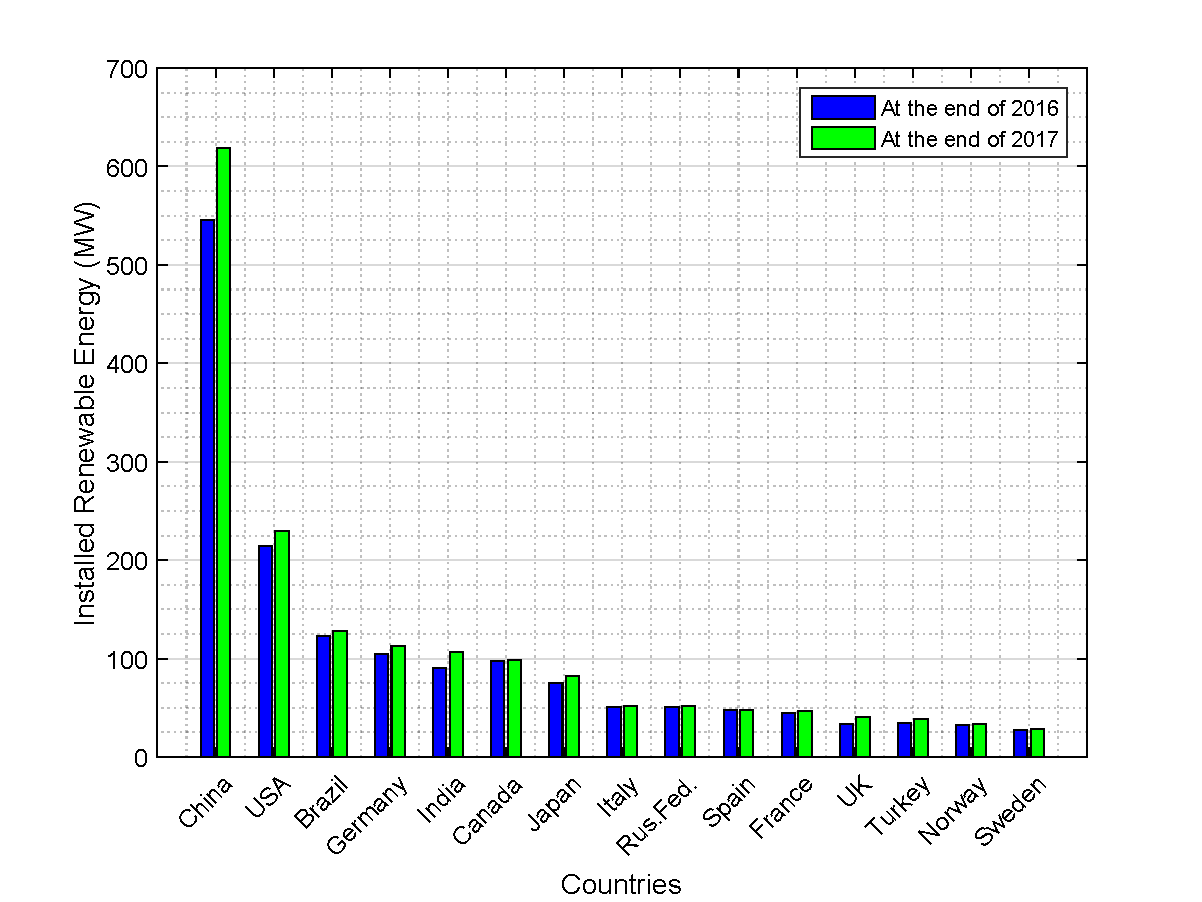
\includegraphics[scale=0.6]{renewablecapacities.pdf}
	\caption{Installed Renewable Energy Capacity of Leading Countries \cite{InternationalRenewableEnergyAgencyIRENA2018},\cite{InternationalRenewableEnergyAgency2017}}
	\label{renewablecap}
\end{figure}
EU countries promote the renewable energy systems from the very beginning. In 2008, two key main targets are set for 2020 by the European Council\cite{EuropeanCommission2008}: 
\begin{itemize}  
	\item At least 20 \% reduction in greenhouse gases (GHG) by 2020
	\item Achieving 20\% renewable energy share in energy consumption of EU by 2020
\end{itemize}
In order to accomplish these targets, the Renewable Energy Directive was published in 23 April 2009. This directive has set national binding targets for EU countries in order to accomplish the 20\% renewable energy target for EU and 10 \% target for the renewable energy usage in the transport \cite{EuropeanParliament2009}. In order to achieve the 20 \% target, each member state determined their own targets ranging from 10\% in Malta to 49\% in Sweden. According to the latest released report by Eurostat, renewable share of the EU in energy consumption has reached 17 \% in 2016 \cite{States2016}. Moreover, eleven of EU member states have already achieved their 2020 targets. Therefore, these ambitious targets imply that the increase in the renewable share will increase continuously.\par
Wind power has the highest share among the renewable energy sources in the installed renewable energy capacity except for hydro power. The wind power capacity at the end of 2017 has reached 514 GW worldwide\cite{InternationalRenewableEnergyAgencyIRENA2018}. The installed wind power capacity of the leading countries is shown in the Fig. \ref{windcap}. As in the case of total installed renewable energy capacity, China and USA have the highest installed capacities in the wind power capacity. \par
\begin{figure}[h!]
	\centering
	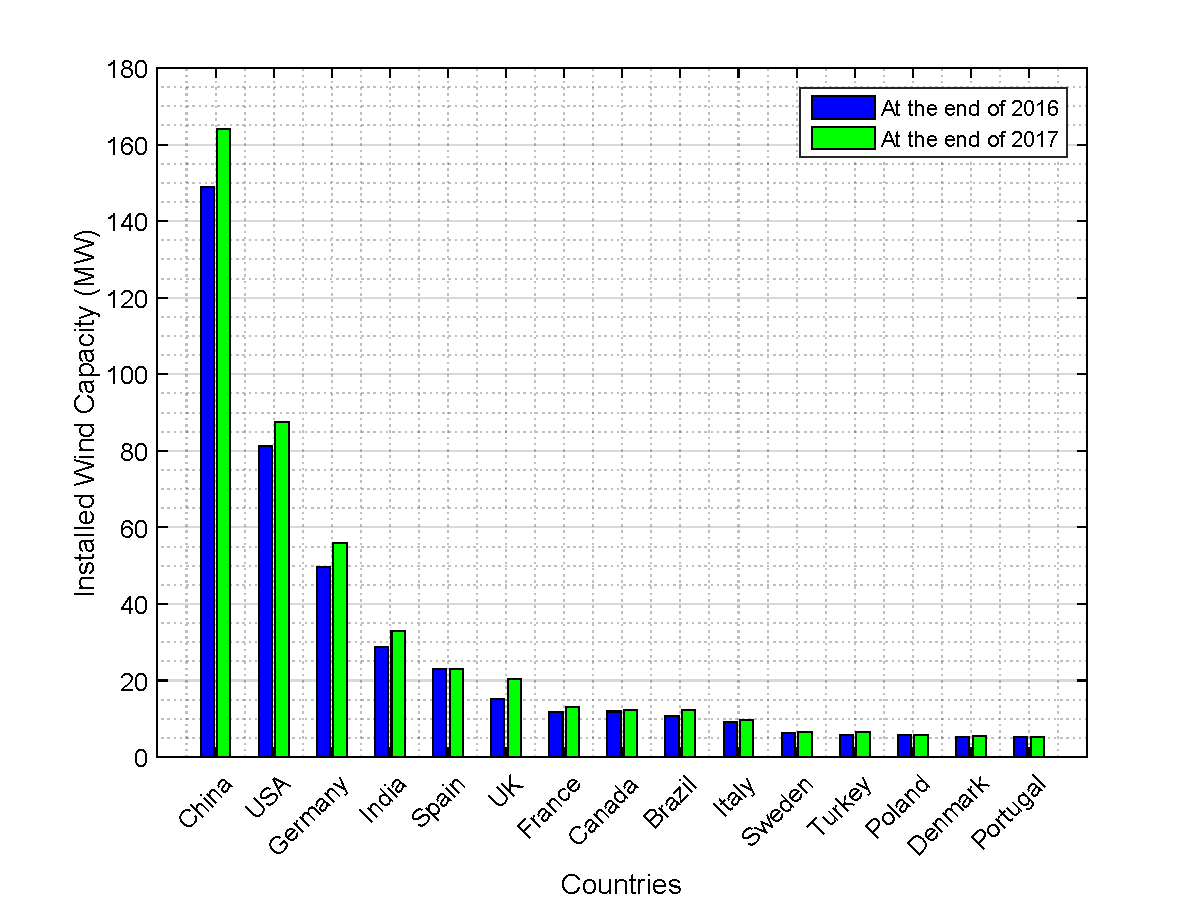
\includegraphics[scale=0.55]{windcapacity.pdf}
	\caption{Wind Power Capacity of Leading Countries in 2016 \cite{InternationalRenewableEnergyAgencyIRENA2018},\cite{InternationalRenewableEnergyAgency2017}}
	\label{windcap}
\end{figure}
The share of renewable energy is increasing continuously. Today, the discussion is about whether 100\% renewable energy is possible in the upcoming future. In \cite{REN212017d}, grid integration issues of wind and solar systems and the lack of sufficient storage technologies are considered as the main barrier for this target meanwhile the major problem seems as the existing energy industry. Nonetheless, a significant renewable share is expected even though the 100\% is realistic or not. The report published by IRENA (International Renewable Energy Agency) estimates the share of renewable energy in EU as 24\% by 2030 which is below proposed target of 27\%\cite{IRENA2014}. Nonetheless, the increase in the renewable energy share will continue in the upcoming future. \par
 
\section{Renewable Energy Problems}
It is an undeniable fact that renewable energy systems are advantageous in terms of global warming and carbon dioxide emission. Nonetheless, they also have disadvantages to the system operators due to intermittent energy generation profile. First of all, the term intermittent in the literature is related to the variable and uncontrollable nature of the renewable sources \cite{KlingeJacobsen2010}. Since the source of the Renewable Energy Sources (RES) is variable, it is not possible to adjust its output according to the demand. Therefore, the thermal plants have to be in the operation when high wind speeds and solar radiation exist. Moreover, the system requires additional start-ups and active power rise from partly loaded plants in order to balance the energy in the system because of the uncertainty of RES. These all create additional costs caused by high share of RES in the system \cite{Zipf2013}. Besides, power grid will face with transmission system issues as overloaded transmission lines, changes on the protection and control in the distribution system, greater level of power-factor control and low voltage ride-through (LVRT) requirements when the RES share is increased in the grid \cite{Ipakchi2009}.\par
Another challenge of increasing RES is the problem of power system frequency stability. Since the frequency of the power system depends on the balance between generation and consumption, grid operators are responsible for adjusting the generation in order to maintain a constant frequency. However, the renewable energy generation is strictly dependent on the renewable source i.e. solar radiation or wind speed. Therefore, renewable systems make the system operation harder due to their intermittent and uncertain power generation profiles. \par 
Frequency of the grid depends on the balance between supply and demand. As the balance is established, frequency stays constant. However, that is the ideal case. In fact, the load always varies. 
It is the responsibility of the grid operator to provide continues balance. Consequently, the grid frequency varies around the nominal frequency with small deviations. However, unintentional generation unit outages or instant load connections cause high deviations in the grid. A generic frequency disturbance is depicted in the Fig. \ref{freq2}. In the beginning of the disturbance, frequency falls with a slope that is called Rate of Change of Frequency (RoCoF) until the minimum frequency what is called frequency nadir is reached. Grid RoCoF is limited with the inertia of the generators. The higher grid inertia decreases RoCoF and increases the frequency nadir. \par
\begin{figure}[h!]
	\centering
	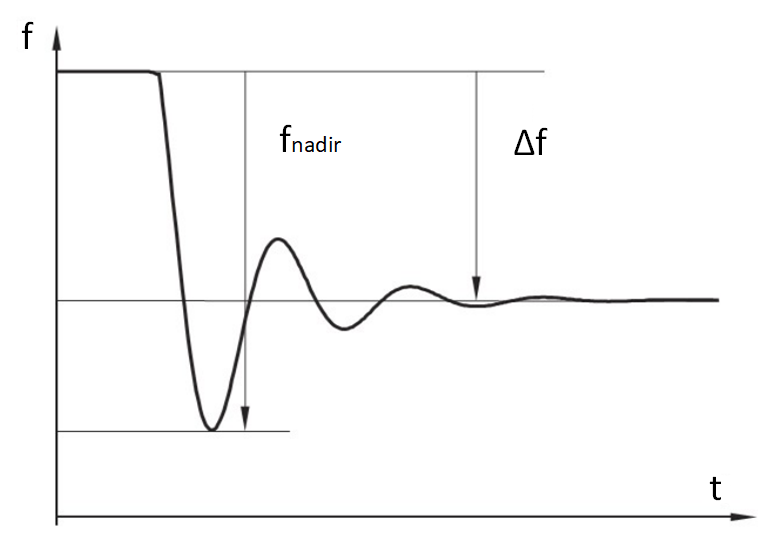
\includegraphics[scale=0.4]{freq2.png}
	\caption{A Generic Frequency Disturbance}
	\label{freq2}
\end{figure}
As the renewable systems with power electronics interface increase in the electricity grid, the grid equivalent inertia decreases. In \cite{Gautam2011}, the reduced grid inertia due to the high DFIG wind turbine penetration is emphasized. Moreover, the results of the reduced grid inertia following a disturbance are listed as: 
\begin{itemize}
	\item increased effective aggregated angular acceleration of synchronous machines which require high restoring forces
	\item high RoCoF and hence, decreased frequency nadir
\end{itemize}
It should be noted that this problem is not specific to DFIG wind turbines but renewable energy systems which are connected to the grid with power electronics. Conventional synchronous generators rotate at synchronous speed which is proportional to the grid frequency. If the grid frequency decreases, then the synchronous speed also decreases. In this case, the generator active power is increased inherently due to kinetic energy extraction from the generator inertia. The increase in active power provides action time for primary controllers and is crucial for frequency stability. \par
Different turbine topologies give different reactions to the frequency disturbances. Wind turbine generator topologies are shown in Fig. \ref{windtop}. Type-1 turbines are connected to grid with a asynchronous generator. The wind turbine generates active power as turbine rotates faster than synchronous speed. Therefore, the generator operates at the linear part of the torque-slip curve. Hence, the change in the grid frequency causes smaller decrease in the turbine speed. Type-2 is very similar to Type-1 except for the variable resistor which can shift the torque speed curve slightly. Hence, the frequency deviations affect the active power output of Type-1 and Type-2 \cite{Muljadi2012}. Type-3 wind turbines include Doubly-Fed Induction Generator (DFIG). DFIG stator is directly connected to grid meanwhile its rotor is connected to grid with a Partial Scale Power Converter (PSPC). Even though the stator is directly coupled to grid, the power electronics enable wind turbine to operate in a range of speeds. Therefore, the rotor frequency is also decoupled from grid.\par
\begin{figure}[h!]
	\centering
	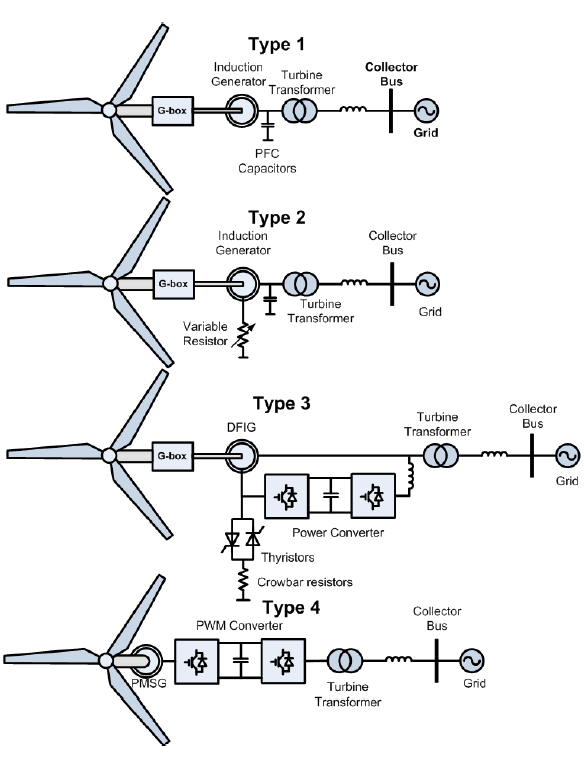
\includegraphics[scale=0.67]{windgentop.png}
	\caption{Wind Turbine Generator Configurations \cite{Muljadi2012}}
	\label{windtop}
\end{figure}
Type-4 wind turbines are connected to grid with back-to-back converters i.e. FSPC. AC/DC and DC/AC conversion decouples the grid frequency and the turbine speed. Due to the decoupling, Type-3 and Type-4 turbines can operate at the MPPT speed that capture the maximum power from air. Nonetheless, this results that Type-3 and 4 wind turbines are not affected from the grid frequency deviations. Therefore, these systems have no contribution to the grid inertia despite the fact that these systems include significant inertia. Hence, the aggregated grid inertia is reduced with the penetration of wind turbines with power electronics. \par
The comparison for different types of generators is made in \cite{VanDeVyver2016} and listed in Table \ref{generatorcomparison}. When the conventional synchronous generator is selected as reference, the fixed induction generator is marked as '+' meaning that it is affected by the grid frequency deviations. However, the grid frequency deviations have small impact on the rotational speed of the generator that decreases the inertial support behaviour. Moreover, DFIG wind generator is marked as '-' meaning that the speed of the generator is disturbed but no inertial support is provided. In this case, PSPC regulates the generator speed. Finally, the wind turbines with FSPC have no inertial response since the generator frequency is fully decoupled from grid frequency.
\begin{table}[h!]
	\centering
	\begin{tabular}{lc}
				\hline
		\multicolumn{1}{c}{\textbf{Type of the generator}}                                                                            & \textbf{Inertial Response Behavior} \\ \hline
		Conventional Synchronous Generator                                                                                            & ++                                   \\
		Fixed Speed Induction Generator (FSIG)                                                                                        & +                                    \\
		Doubly Fed Induction Generator (DFIG)                                                                                         & -                                    \\
		\begin{tabular}[c]{@{}l@{}}Variable Speed Wind Turbine Generator\\ (with Full Scale Power Electronics)\end{tabular} & None                                 \\ \hline
	\end{tabular}
	\caption{Comparison of Different Types of Generators for Inertial Response Behaviour}
	\label{generatorcomparison}
\end{table}
Another reason for the decrease in the grid inertia is the de-commitment or dispatch of the conventional sources due to economic concerns. Since the renewable energy systems have the lowest cost for energy production, they are preferred instead of conventional generators in the economical dispatch. As a result, conventional generators are dispatched to a lower generation profile or taken-off from operation.\par
It should be noted that grid inertia is directly related to the amount of load in the system in addition to the share of RES. Since the amount of online generators fluctuate within time, the grid aggregated inertia also changes. Hence, the scenario in which the system has low demand and also high renewable generation is the most critical one since the lowest grid inertia exists in the network.\par
In brief, the main problem that comes with increasing RES penetration is the reduction in the grid effective inertia. If the share of the RES increases continuously, the existing grid will be exposed the higher RoCoF and lower frequency nadir in the future. The solution of this problem is the emulation of the synchronous generator inertial support behavior on the RES. However, the capability of the wind turbine for inertial support behavior is not revealed for varying wind speeds. This thesis study focuses on the investigation of the inertial support limits on the wind turbines with FSPC in order to maximize the support power. Besides, the economical perspective of the inertial support is also examined from the energy provider perspective. In this way, the feasibility of the inertial support is also studied by focusing on the payment methods of the grid supporting applications. Consequently, maximum performance can be obtained from wind turbines that enables the power grid increasing the share of RES without causing frequency stability problems to grid operators.
\section{Literature Review}
Studies regarding inertial support date back to early 2000s. In the study \cite{Lalor2004}, the effect of the increasing wind energy penetration is investigated. The study concludes that increasing share of wind energy increases the primary reserve requirement for the successful grid operation. The increased frequency deviations, especially in light load conditions (high wind generation with low consumption scenario) can be mitigated in the system as long as the wind generation provides inertia support. Study in \cite{Ekanayake2003} states that DFIG wind turbines are decoupled from power system resulting in no contribution to system inertia. A supplementary loop is proposed for reinstating the machine inertia. Moreover, in \cite{Ekanayake2004}, performance of the  supplementary control loop is evaluated with the comparison of the inertial support of a fixed-speed wind turbine. The proposed control loop which is shown in Fig. \ref{inertiacontrol} is validated in \cite{Morren2006} and compared with the droop control in \cite{Morren2006a}.\par
\begin{figure}[h!]
	\centering
	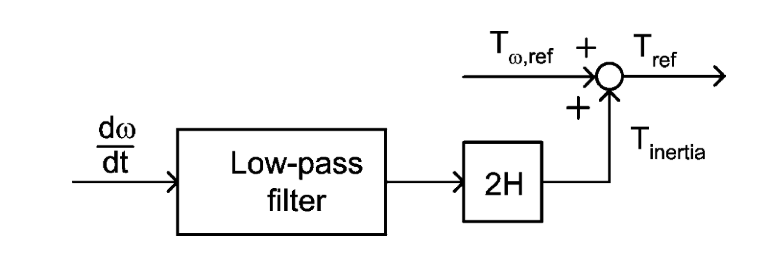
\includegraphics[width=.65\linewidth]{inertiacontrol.png}
	\caption[Inertia Controller]{Inertia Controller in \cite{Morren2006a}}
	\label{inertiacontrol}
\end{figure}
It is an undeniable fact that renewable energy systems are the most economical way of producing electrical energy due to absence of any fuel cost. Therefore, they are to be operated in their rated power. If they are required for the primary frequency control, the wind turbine active power should be curtailed. In this way they can leave a margin for droop control. Droop control by wind energy systems is also studied in the literature. In \cite{Muljadi2012}, the inertial support of different types of wind turbines is compared. It is concluded that the Type-4 wind turbines are able to perform better performance for inertial support due to the power electronics interface. Moreover, combination of inertial support and droop control produces better results in these wind turbines.\par
Inertial support by utilizing the kinetic energy in the turbine is proposed in literature with two main methods. One of the methods is increasing the active power by a defined percentage and it is presented in literature with different names such as Fast
Inertial Support, Fast Power Reserve or Stepwise Inertial Control. In this type of support, the support power is released with a step increase in the active power. In \cite{Hansen2014}, the fast inertial support is proposed with predefined increases in the active power. Nevertheless, the converter ratings and the effect of the wind speed in the fast inertial support capability are not emphasized. \par
The second proposed method is the active power increase proportional to grid RoCoF. The method is called in literature as synthetic inertia control, hidden inertia control or
virtual inertia. Actually, synthetic inertia is a method not only for wind turbines but converter interfaced systems to emulate synchronous generators. In \cite{Zhu2013a}, the method is implemented a VSC-HVDC system in order to improve frequency stability of a weak grid. Study \cite{Hernandez2017} focuses on the implementation in the PV systems in coordination with energy storage systems. In \cite{Zhu2018a}, the synthetic inertia implementation is studied with cooperation with Lithium-Ion supercapacitors. \par
In the studies \cite{VanDeVyver2016},\cite{Conroy2008},\cite{Gonzalez-Longatt2013}, the synthetic inertia controller is implemented on a variable speed wind turbines. The active power output of the wind turbine is changed according to the grid RoCoF as shown in the Fig. \ref{inertiacontrol2}. The effects of the synthetic inertia implementation in a full-scale wind turbine are studied in \cite{Gonzalez-Longatt2013}. A variable synthetic inertia controller is proposed in \cite{Bonfiglio2019} that improves the speed recovery of the wind turbine. Nonetheless, the better speed recovery is achieved at the expense of the longer speed recovery time. \par
\begin{figure}[h!]
	\centering
	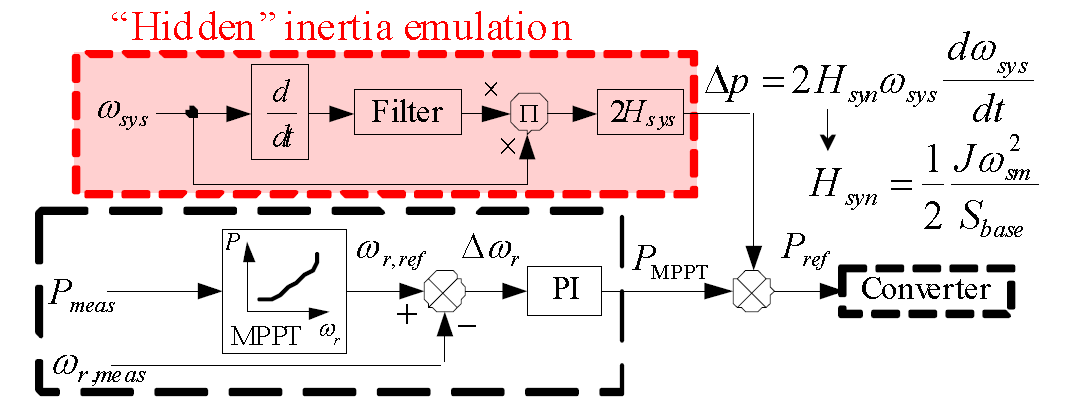
\includegraphics[width=.8\linewidth]{inertiacontrol2.png}
	\caption{Hidden Inertia Controller in\cite{Gonzalez-Longatt2013}}
	\label{inertiacontrol2}
\end{figure}
The modern wind turbine manufacturers also study the inertial support capability for their wind turbines. General Electrics has active power control module called as WindINERTIA for their wind turbines in order to react the large frequency disturbances. The control module can increase the power output of the wind turbine by 5-10\% for a few seconds (10\% for 15 seconds) \cite{Clark2009}. The control diagram of the module is shown in Fig. \ref{inertiacontrolge}. Moreover, Enercon provides inertial response capability to the turbines by allowing 10\% increase in the active power\cite{Enercon2018}. Nonetheless, solutions of GE and Enercon are independent of the grid RoCoF.\par
\begin{figure}[h!]
	\centering
	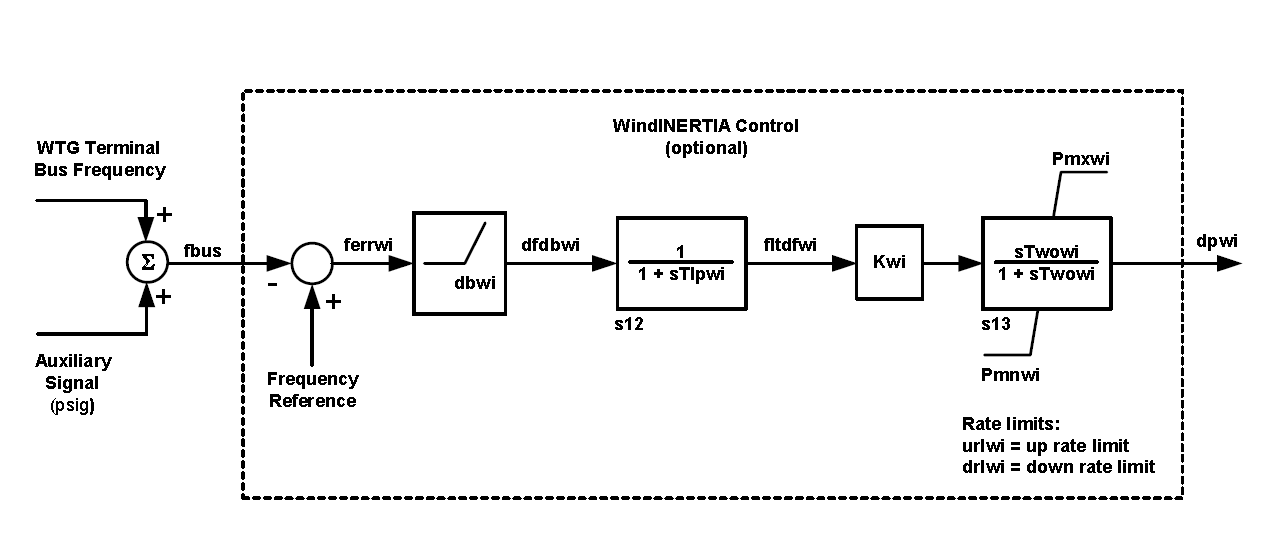
\includegraphics[width=.95\linewidth]{inertiacontrolge.png}
	\caption{GE WindINERTIA Control Diagram in \cite{Clark2009}}
	\label{inertiacontrolge}
\end{figure}
However, the full capacity of the wind turbines for inertial support is not studied in literature. Practical limits of the inertial support are studied in \cite{Gonzalez-Longatt2016} by varying the inertia constant to be emulated. The study focuses the emulation of higher inertia constants without consideration of the wind speed in the support time. The practical limits in terms of maximum achievable power and turbine internal parameters are not focused in the study. Finally, the studies in literature do not investigate the practical limits of the wind turbine. By investigating full capacity of the wind turbine, the importance of the wind turbines for frequency stability studies can be emphasized. 
\section{Thesis Motivation}
Although renewable energy systems are beneficial for environmental concerns and the absence of fuel cost, higher renewable penetration also brings operational challenges for system operators. One of the most important problems that comes with renewable energy is the deterioration on the power system frequency stability. With the high renewable penetration, grid aggregated inertia decreases. As a result, grid is exposed to high rate of change of frequency (RoCoF) for the disturbances in heavily renewable penetrated systems. This implies that the successful operation of power systems with increasing renewable energy penetration is not achievable unless the decrease in the grid inertia is prevented. Therefore, the main objective of this study is to avoid the decrease in the grid inertia arising with the renewable energy penetration. In this way, the share of renewable energy systems can be increased without the negative effects on the power system operation.

%To avoid steeper frequency declines in the grid, all generation technologies should provide inertial support for the frequency disturbances.\par
Wind energy systems, especially variable speed wind turbines with full scale power electronics are the most promising renewable energy systems that can contribute to grid frequency stability due to the high inertia in their blades and generator and also their back-to-back converters that give ability to control its active power. Wind turbine with full-scale power electronics is the key solution to be used against the decrease in the grid inertia. However, the full capability of a wind turbine with full-scale power electronics has not been discovered yet. This study will explore the full capacity of the wind turbines for the inertial support. The practical limits of the wind turbines are explored under different wind speed scenarios. Another objective of this study is revealing the effects of grid supporting functions in the wind turbines. Besides, the differences between the frequency dependent and independent inertial support mechanisms are investigated especially for weak power systems.
%The knowledge of the wind turbine inertial support capability enables the grid operator to build new frequency regulating mechanisms. In this way, the participation of turbines for these mechanisms can be encouraged. \par
%Inertial support methods (either dependent on frequency or not) are presented in the literature. However, comparison of their performances under a weak power grid has not studied. This study aims to find out which type of inertial support is efficient for weak power grids. \par
%In Turkey, renewable energy systems produce electricity through the feed-in tariff that is the guaranteed price to these systems. Hence, the energy providers would not be volunteer for inertial support implementation unless system operators make this service mandatory or the implementation has economical benefits. The results of this thesis will present a basis for economical analysis by the energy provider perspective.
\section{Thesis Outline}
This thesis study focuses on the wind turbine inertial support limits and its effects on power system stability. The thesis starts with a brief summary of the renewable energy status in Chapter \ref{chp:1}. By reviewing the share of the renewable energy systems and the targets for upcoming future, the importance of the frequency stability studies is highlighted. Moreover, renewable energy problems and the proposed solutions in literature are presented. \par
In Chapter \ref{chp:2}, the frequency concept in power systems is extensively described. Since renewable energy systems are replaced or preferred over the conventional power generation units, the electricity grid is facing with frequency stability issues due to the absence of inertia-less units. Therefore, the behaviur of old-fashion power plants are described under frequency disturbances. Moreover, the frequency regulating mechanisms are presented. Finally, the energy markets are also explained in order to emphasize the position of renewable energy systems.\par
Chapter \ref{chp:3} presents the modelling of wind turbine used in this study. Since the existing variable speed wind turbines require modification in order to integrate to electricity grid, detailed modelling of these wind turbines is presented. By utilizing synthetic inertia method, a relation between grid frequency and the active power output is constructed.\par
The limits of the active power increase are investigated in Chapter \ref{chp:4}. The ability of increasing its active power output is already presented in literature. However, the limits of support power are studied for different wind speed scenarios. The real wind speed measurements from site are utilized to find the probability of support power for different wind speeds. Wind turbine inertial support limits and turbine internal parameters are observed for the non-dynamic frequency response.\par
Synthetic inertia implementation is the implementation of inertial support behavior on RES by establishing a relation between grid RoCoF and turbine active power output. The implementation on a wind farm is studied in Chapter \ref{chp:5}. The effect of synthetic inertia is observed in a dynamic test case with renewable penetration. Test case is modified with different combinations in which the system is penetrated with wind farm with/without generator decommission are studied in this chapter. Frequency response of the test system is tested for different grid configurations as well as different emulated inertia constants. Furthermore, the synthetic inertia implementation is evaluated for the Turkish electricity system. \par
Chapter \ref{chp:6} evaluates the effects of the fast inertial support and synthetic inertia implementation. Moreover, an economical analysis from an energy provider perspective is given. Two hypothetical payment methods are constructed and compared to estimate which economical motive can convince the energy provider for participating grid supporting methods with renewable energy systems. \par
Chapter \ref{chp:7} presents a basic conclusion for the inertial support implementation which is either frequency dependent or not. The contribution of the thesis study on the grid inertia reduction is emphasized by reviewing the inertial support capability of the wind turbine especially for low and medium wind speeds. Moreover, the feasibility of the inertial support implementation is investigated in terms of the payment methods.


















% CHAPTER 1
\chapter{POWER SYSTEM FREQUENCY STABILITY}
\label{chp:2}
The increasing renewable energy penetration deteriorates the power system frequency stability. One of the most severe effect of renewable energy penetration is the reduction in grid inertia. Grid aggregated inertia is important for the frequency stability. As the frequency falls, a part of the kinetic energy is extracted from the grid inertia and released inherently from synchronous generators to grid. Therefore, as the grid aggregated inertia decreases, the control of the frequency becomes difficult resulting in quick changes in the grid frequency.\par
In this chapter, the internal dynamics of the power system will be presented in terms of frequency stability. The frequency regulation mechanisms in the grid is presented. Furthermore, the energy market is briefly explained in order to understand the role of renewable energy providers inside the market.
\section{Synchronous Generator and Synchronous Speed}
Synchronous machines produce torque only in synchronous speed. If a transient over-speeding occurs in the rotor, the torque cannot be produced that results in a deceleration. This makes the rotor angular velocity to strictly coupled to the electrical frequency  of the stator rotating MMF. This is why these machines are equipped with damper windings which are basically induction machine windings. If the frequency of  grid changes, damper windings create a torque which creates a force to synchronize the speed to the grid frequency. \par
\begin{equation}
n_{s}=\frac{120f}{p}
\label{syncspeed}
\end{equation}
Relation between grid frequency and the synchronous speed is given in Eq. (\ref{syncspeed}) in terms of rpm where $n_{s}$ is the synchronous speed in rpm, $f$ is the grid frequency in Hz, $p$ is the number of poles of the generator \cite{Kundur}.

\section{Swing Equation}
\label{swing}
Rotational speed of synchronous machines changes according to the net torque acting on the rotor. Therefore, the speed is maintained constant unless there is a difference between mechanical and electromechanical torque. The equation of motion is given in Eq. (\ref{eqmotion}) where $J$ is aggravated moment of inertia of the generator and the turbine in $kgm^{2}$, $\omega_{m}$ is the rotor angular velocity in $rad/s$, $T_{m}$ and $T_{e}$ are mechanical and electromechanical torques in $Nm$. $T_{a}$ is the accelerating torque in $Nm$ which determines the acceleration or deceleration in the rotor according to its sign.
\begin{equation}
J\frac{d\omega_{m}}{dt}=T_{m}-T_{e}=T_{a}
\label{eqmotion}
\end{equation}
In power system network, the power ratings of the generators in operation and corresponding moment of inertia values varies. Inertia constant is defined as the ratio of kinetic energy stored in the inertia to the power rating of the generator as in Eq. (\ref{inertiaconstant}) where $\omega_{0m}$ denotes the rated angular velocity of generator in $rad/s$ and $S_{base}$ is the rated apparent power in $VA$. $H$ is indicates the time duration in which generator produces its rated apparent power by only using its kinetic energy in the inertia. Thus, $H$ is a better indication of factor for power system frequency stability analysis compared to $J$. Hence, it is more convenient to use inertia constant, $H$ which varies between 2 and 9 seconds \cite{Kundur}.
\begin{equation}
H=\frac{{\frac{1}{2}}J\omega_{0m}^{2}}{S_{base}}
\label{inertiaconstant}
\end{equation}
Substituting Eq. (\ref{inertiaconstant}) into Eq. (\ref{eqmotion}) and replacing units to per-unit quantities yield the swing equation given in Eq. (\ref{eqmotion5}) where $\overline{P_{m}}$ is the input mechanical power in pu and $\overline{P_{e}}$ is the electromechanical output power in pu. It defines the inherent behaviour of a synchronous generator against the frequency deviations in the grid. When the grid frequency falls, a subsequent decrease in the rotor is observed. According to the Eq. (\ref{eqmotion5}), a negative term is found in the left-hand side. This means that rotor electromechanical output power, $\overline{P_{e}}$ will be increased inherently. It should be noted that the additional energy is not taken from the input mechanical power but it is extracted from the kinetic energy. Moreover, the decreased energy is injected to grid whenever the frequency increases due to the acceleration in the rotor.
%\begin{equation}
%J=\frac{2H}{\omega_{0m}^{2}}{S_{base}}
%\label{inertiaconstant2}
%\end{equation}
%\begin{equation}
%\frac{2H}{\omega_{0m}^{2}}{S_{base}}\frac{d\omega_{m}}{dt}=T_{m}-T_{e}
%\label{eqmotion2}
%\end{equation}
%\begin{equation}
%\frac{2H}{\omega_{0m}^{2}}{S_{base}\omega_{m}}\frac{d\omega_{m}}{dt}=P_{m}-P_{e}
%\label{eqmotion3}
%\end{equation}
%\begin{equation}
%2H\frac{\omega_{m}}{\omega_{0m}}\frac{d(\omega_{m}/\omega_{0m})}{dt}=\frac{P_{m}-P_{e}}{S_{base}}
%\label{eqmotion4}
%\end{equation}
\begin{equation}
2H\overline{\omega_{m}}\frac{d\overline{\omega_{m}}}{dt}=\overline{P_{m}}-\overline{P_{e}}
\label{eqmotion5}
\end{equation}
\section{Frequency in Power Systems}
The frequency in a power system is related to the speed of the synchronous generators and changes according to the swing equation. The frequency of the each generator is not the same in the network since each generator does not have the same speed. Nonetheless, the fluctuations in the generator speeds are called rotor swings and can be negligible in the steady state. Hence, the network can be assumed as a single generating unit by neglecting small differences between the generator speeds. The swing equation basically investigates the relation between mechanical and electromechanical powers and the rate of change of angular speed of a generator. However, it is also applicable to grid in order to estimate the grid frequency.\par
\begin{equation}
\label{systemswing}
2H_{sys}\overline{f}_{sys}\frac{d\overline{f}_{sys}}{dt}=\overline{P}_{tm}-\overline{P}_{te}
\end{equation}
If the generators of the grid is considered as a single generator, the inertia of the equivalent generator is aggravated from each generator in the network. In this case, average frequency in the network can be found as in Eq. (\ref{systemswing}) where $P_{tm}$ is the aggravated mechanical input power of the generators meanwhile $P_{te}$ is the aggravated electromechanical output power. In other words, the system frequency depends on the balance between generation and consumption. It should be noted that generation means the input mechanical power of the generators meanwhile the demand is absorbed from the electromechanical output power of the generators. Hence, the difference between these causes either acceleration or deceleration. \par
\begin{figure}[h!]
	\centering
	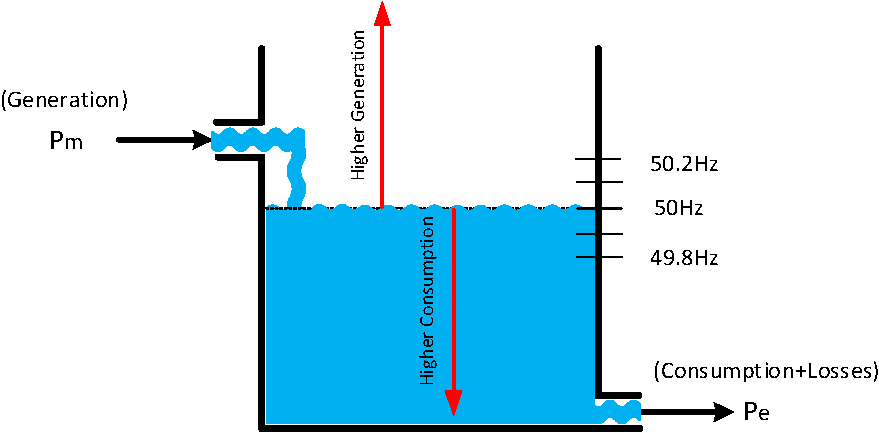
\includegraphics[width=.9\linewidth]{frequencypool.pdf}
	\caption{Frequency behaviour in electric grid with the water level in a container analogy \cite{Eto2010}}
	\label{frequencyingrid}
\end{figure}
The behaviour of the frequency in electric grid is depicted in Fig. \ref{frequencyingrid}. As it can be seen from the water level in a container analogy, the frequency of the system is dependent on the in-flow and the out-flow. Therefore, in the electricity grid, frequency increases as the aggravated input power is higher than the aggregated output power. Note that, the direction of the frequency is dictated by this balance. Having a constant 49.8Hz frequency does not mean that consumption is higher than generation. If the frequency is constant, then the input mechanical power is equal to output power.\par
The variation of the grid frequency is depicted for a typical day in Fig \ref{06decfreq}. The frequency deviates continuously during the day. It should be noted that there exists hourly peaks in the frequency. The peaks occur due to the change in the hourly generation shift. Since the generation level is changed for the next hour, the frequency deviates hourly in the grid.
\begin{figure}[h!]
	\centering
	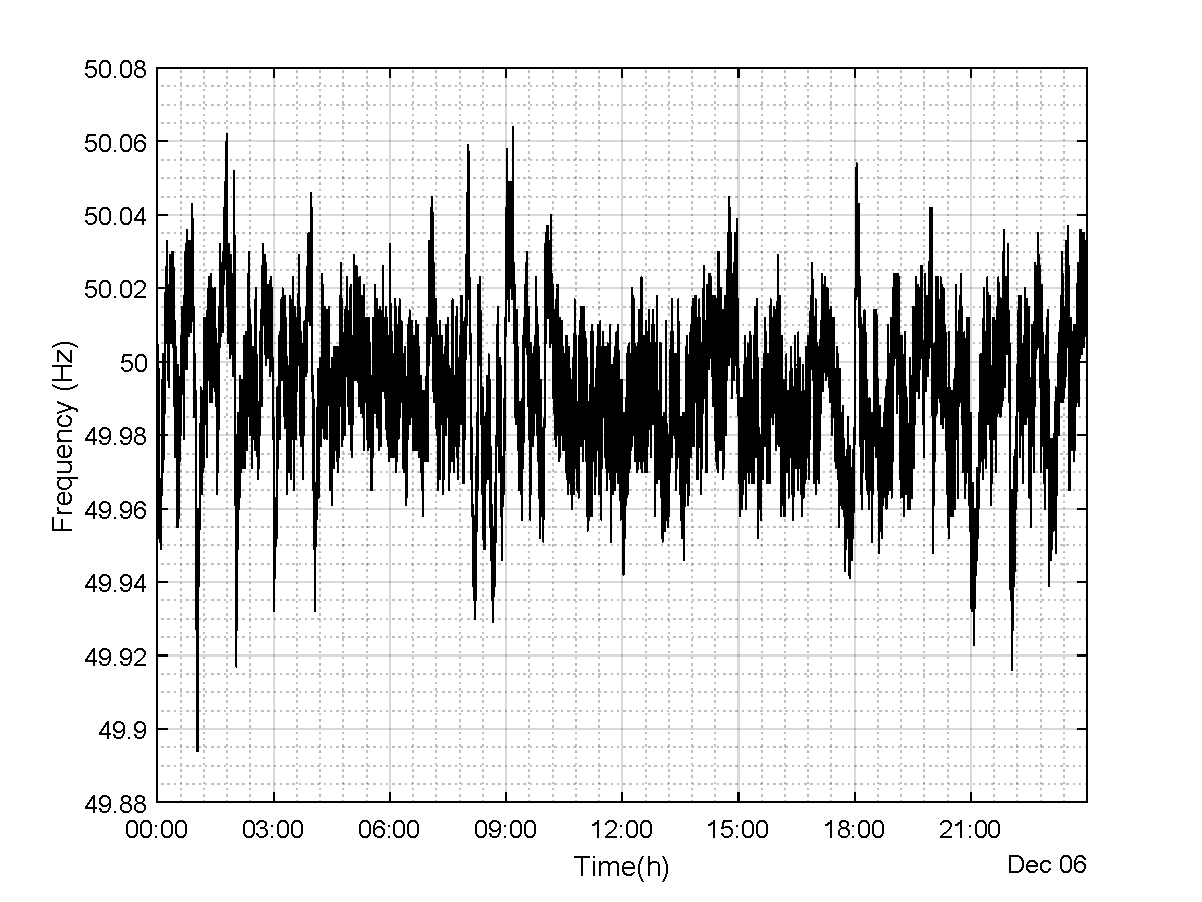
\includegraphics[width=.9\linewidth]{06decfreq.pdf}
	\caption{Variation of the Frequency in a Typical Day (06 Dec 2018) \cite{teiasfreq}}
	\label{06decfreq}
\end{figure}
\section{Frequency Regulating Mechanisms}
Having a constant frequency is one of the most important responsibilities of a system operator. In order to have a constant frequency, supply is being adjusted according to the demand continuously. By doing so, the system frequency varies between a band-gap. The variation depends on the disturbances which are generally a sudden generation outage or instant load connection. The size of the disturbance determines the severity of the frequency change and there are three main mechanisms to arrest the frequency changes in the system. \par
The frequency control services in England and Wales are depicted in Fig. \ref{freqcontrol} for a frequency disturbance. The frequency is maintained between 49.8Hz and 50.2Hz for continuous service. A frequency disturbance event causes frequency to decline. However, the decline in the frequency is arrested with the help of the inertial support of the conventional generators and the primary frequency controllers. The main responsibility of the primary frequency control is arresting the frequency decline. Restoration of grid frequency to nominal is the responsibility of the secondary and tertiary frequency controls.
\begin{figure}[h!]
	\centering
	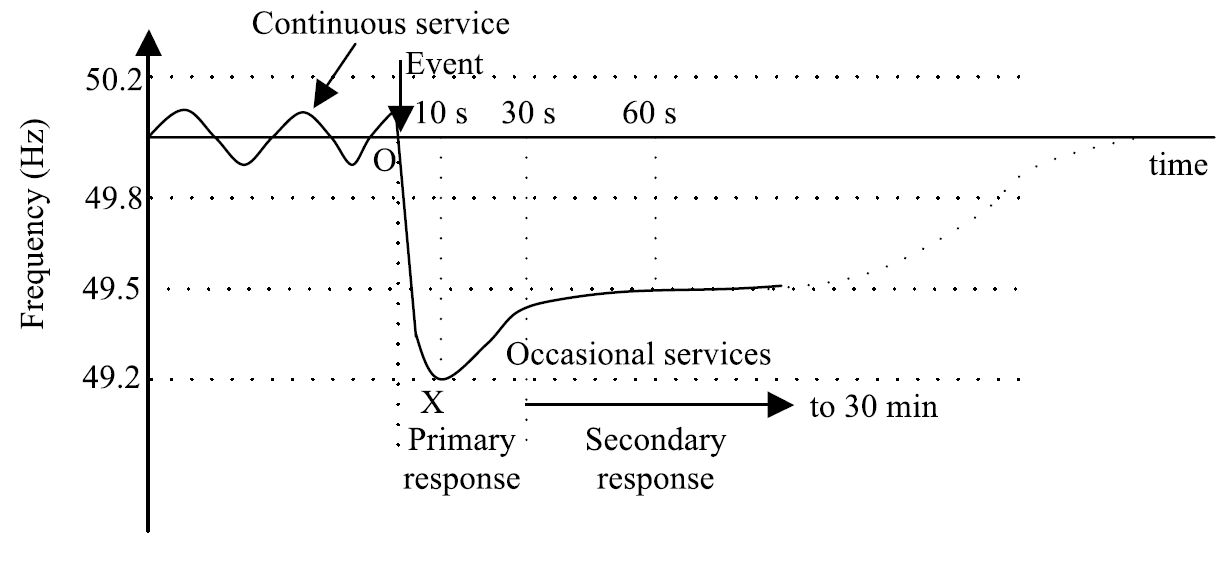
\includegraphics[scale=0.35]{freqq.png}
	\caption{Grid Frequency Control in England and Wales \cite{Ekanayake2008}, \cite{Erinmez1999}}
	\label{freqcontrol}
\end{figure}
\subsection{Primary Frequency Control}
Following generator outage or sudden load connection event, frequency starts decreasing. The rate of change of the frequency is dependent on the severity of the event by means of power and the available inertia of the power system. Such frequency disturbance requires increased input power. However, the increase in the input mechanical power should be activated very fast and should be automated. This responsibility is assigned to generating units with primary frequency control. The active power generation of these units is increased or decreased by the governor depending on the network frequency direction. Notice that each generator in the power system does not necessarily perform primary frequency control function. In this case, their active power generation is independent from the network frequency. The contribution to primary frequency control is an responsibility but also a way to sell higher energy to grid operator.
The primary frequency control is automated with droop control defined in the generator speed governors. According to droop control, the generator power should be increased according to the frequency deviation from nominal. Therefore, the generating unit does not utilize its whole capacity but rather keeps a capacity which is called as spinning reserve. According to the droop curve, the generation unit should increase its output power no longer than 15 seconds and keep their operation up to 30 minutes\cite{Machowski2011}.
\subsection{Secondary Frequency Control}
The frequency is recovered back to nominal value with the Secondary Frequency Control action. This controller might be a single or multiple centres that monitor the frequency and adjust the generation accordingly. They are also called as Automatic Generation Control (AGC) systems and their action takes a few minutes. The AGC monitors the frequency deviation from the nominal and takes action to recover frequency back to nominal. With the secondary frequency control action, primary controllers decreases their production back to their pre-disturbance value.
\subsection{Tertiary Frequency Control}
The final frequency control mechanism is the Tertiary Frequency Control. If the frequency is not recovered back to nominal value with the secondary controllers, tertiary frequency controllers manually activates the load shedding which is an undesired situation by the network operator. However, it is an emergency case which might result in black-out and requires immediate action.
\section{Energy Market}
Since the energy is generated and distributed by private energy companies, a system operator should be responsible for maintaining a balance in the power network. The frequency is kept inside the operational band in the electricity network by balancing the supply and the demand by intersecting the supply and demand curves inside the different time intervals. In this way, the balance is ensured in the market by day ahead, intra-day and balancing markets. 
\subsection{Day Ahead Market}
The load power in a network has a distinct characteristic depending on the day of the week or the hour of the day. By foreseeing the next day demand power variation, the electricity market collects the bids from the energy suppliers and consumers. According to submitted bids, the next day generation price is determined by intersecting the supply and demand price curves. The price of the energy is called Market Clearing Price (MCP). These bids are submitted for the next day and the prices are determined before the corresponding day.
\subsection{Intra-Day Market}
Even though the estimations for the upcoming day load power has superior accuracy with the advanced estimation methods, networks are subjected to unexpected problems such as generator trips, line outages. Therefore, intra-day market contributes the balance of the market between the day ahead market and balancing market. Moreover, it gives the participants almost real-time trading opportunity meanwhile it increases the sustainability of the market. After day ahead market has closed for the corresponding day, the bids are submitted to system. In other words, MCP is already determined for the corresponding day meanwhile the rest of the day prices are not set. 
\subsection{Balancing Market}
Primary and secondary control reserves are maintained in the system in order to improve the balance for the instant deviations in the frequency. The frequency is first arrested by the primary controllers and it is restored by the secondary controllers. The generation units that participate primary and secondary control promises a defined generation capacity to these actions. Balancing market is much more different than day ahead and intra-day market since its main goal is the network security rather than electricity trading. The price of the energy in this market called as System Marginal Price (SMP).\par
The price of the energy changes according to the market type. In the Fig. \ref{markets}, three market prices such as Market Clearing Price (MCP), Weighted Average Price (WAP) and System Marginal Price (SMP) are shown.
\begin{figure}[h!]
	\centering
	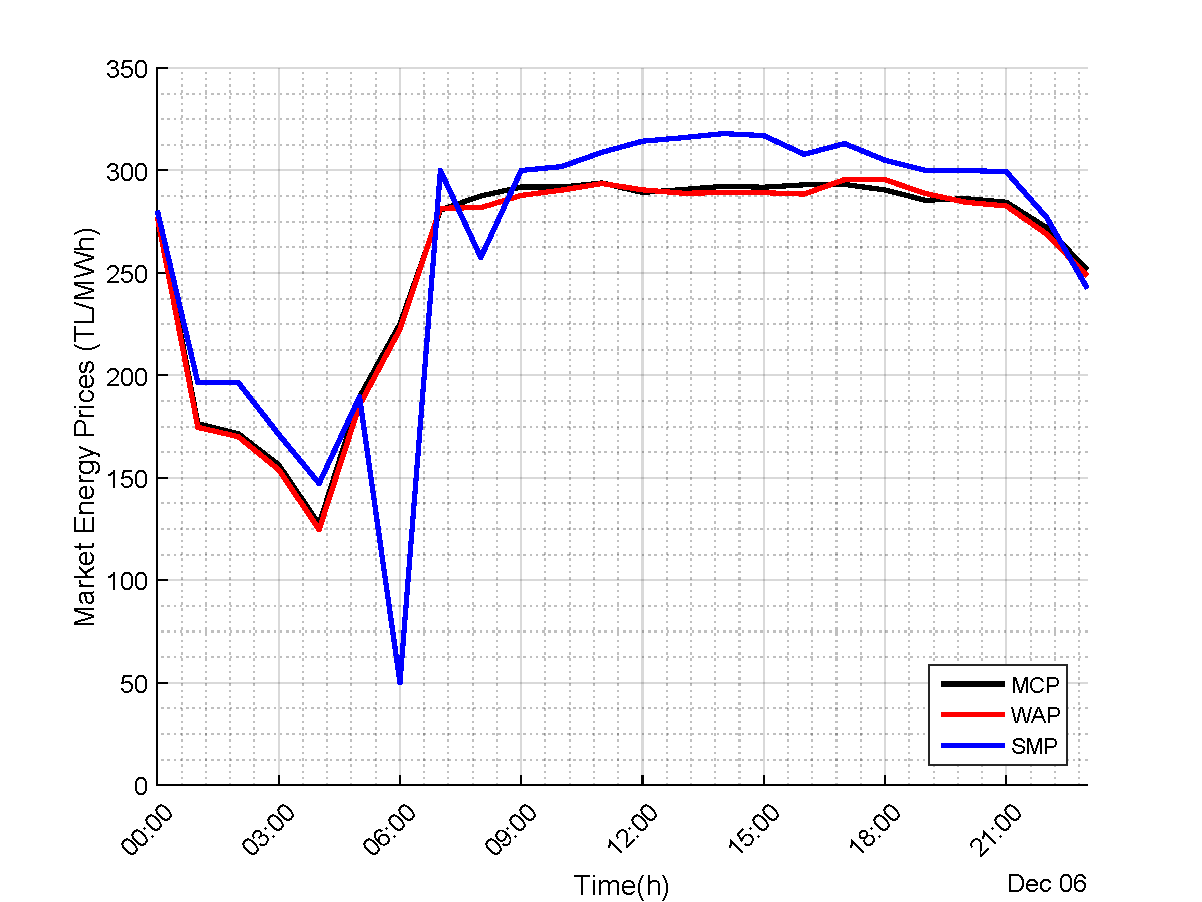
\includegraphics[scale=0.7]{marketprices.pdf}
	\caption{Energy Prices on 06 Dec. 2018 \cite{TEIAS2019}}
	\label{markets}
\end{figure}
\subsection{Feed-In Tariff}
\label{section-price}
Significant amount of energy produced inside the Turkish electricity network is based on exported sources such as coal and gas. As a result of this, the energy sector is highly dependent on the foreign countries. In order to decrease the dependency on the external sources, the renewable energy sources are supported by government in Turkey. The energy generated by renewable energy systems are bought with the feed-in tariff (FIT) within the pre-determined time interval according to the purchase agreement. This decreases the return of investment due to the fact that all produced energy will be bought during this period with a remarkable price. The feed-in tariff for different renewable energy systems is listed in Table \ref{price}.\par
\begin{table}[h]
	\centering
	\begin{tabular}{cc}
		\hline
		\textbf{Renewable Energy System} & \textbf{\begin{tabular}[c]{@{}c@{}}Feed-In Tariff\\ (cent/kWh)\end{tabular}} \\ \hline
		Hydro                            & 7.3                                                                          \\
		Wind                             & 7.3                                                                          \\
		Geothermal                       & 10.5                                                                         \\
		Biomass                          & 13.3                                                                         \\
		Solar                            & 13.3                                                                         \\ \hline
	\end{tabular}
\caption{Feed-In Tariff for Renewable Energy Systems in Turkey \cite{yasa}}
\label{price}
\end{table}
In addition to feed-in tariff, energy provider can benefit from additional incentives as long as some parts of the system is produced inside Turkey. For instance, by preferring the tower of a wind turbine which is a domestic production, an additional price is given to energy provider as local-bonus content. The local-bonus contents for wind turbines are listed in Table \ref{price2}.\par
\begin{table}[h!]
	\centering
	\begin{tabular}{cc}
		\hline
		\textbf{\begin{tabular}[c]{@{}c@{}}Local Content\\ for Wind Turbines\end{tabular}}   & \textbf{\begin{tabular}[c]{@{}c@{}}Local Content Incentive\\ (cent/kWh)\end{tabular}} \\ \hline
		Blade                                                                                & 0.8                                                                                   \\
		\begin{tabular}[c]{@{}c@{}}Generator and \\ Power Electronics\end{tabular}           & 1.0                                                                                   \\
		Turbine Tower                                                                        & 0.6                                                                                   \\
		\begin{tabular}[c]{@{}c@{}}All Mechanical Parts in \\ Rotor and Nacelle\end{tabular} & 1.3                                                                                   \\ \hline
	\end{tabular}
	\caption{Local Content Incentives for Wind Turbines\cite{yasa}}
	\label{price2}
\end{table}
With the increasing renewable energy penetration, the power system stability is getting more vulnerable to the disturbances. Since the grid operators are responsible for the successful operation of the grid, they work on grid stability improving. Nonetheless, power system stability is not the responsibility of the energy providers. However, participation of the renewable energy providers is also a necessity to improve frequency stability of the grid. Hence, the grid operators have to come up with a solution to be implemented by the energy providers. Nonetheless, the solution should also be beneficial for the energy providers who is already satisfied with the existing purchase agreement with additional incentives. As long as the renewable energy providers are convinced to implement the solutions, the grid stability can be maintained against the increasing renewable penetration.
\section{Conclusion}
This chapter focuses on the frequency dynamics inside the power grid. The importance of inherited inertial support of the synchronous generators are highlighted. The characteristics of this behaviour is defined with swing equation that can be adopted to renewable energy systems. The swing equation explains the change in the active powers of the synchronous generators upon a frequency disturbance on the output terminal. However, the internal dynamics of the frequency is also presented to understand the frequency stability. \par
Frequency regulating mechanisms such as primary, secondary and tertiary control are essential for power systems. Their action sequence are also explained in detail. In addition to technical details, the energy market is also summarized to present a economical perspective. 
% CHAPTER 1
\chapter{WIND TURBINE MODELLING}
\label{chp:3}
Ancillary services are getting attention especially for renewable energy systems. Participation of renewable energy systems to frequency regulating mechanisms will be a necessity for the successful operation of the power system. Hence, the detailed modelling of renewable energy systems are essential for grid supporting implementations. In this chapter, detailed modelling for wind turbines is investigated. The wind turbine modelling is presented for the wind turbines that are connected to grid with full-scale power electronics. 
\section{Wind Turbines with Full Scale Power Electronics}
The share of variable speed wind turbines with full scale power electronics is increasing worldwide due to the high efficiency. Full-scale power electronics enables the turbine to have wide speed range. The wind turbines in this type are able to adjust its speed according to the variation in the wind speed and torque \cite{Chen2009b}. PMSG wind turbines are one of the most common type of these turbines. Even though the price of the permanent magnet fluctuates with time, the reliability and high efficiency of this type of turbine increase its share in the market. The wind turbine modelling in this study is based on PMSG wind turbines. However, the ability to control the wind turbine output power is not just specific to PMSG wind turbines but the ones with full-scale power electronics. \par
Fig. \ref{varspeedpmsg_1}, \ref{varspeedpmsg_2} and \ref{varspeedpmsg_3} show the modelling of wind turbine topologies that are connected to grid full-scale back-to-back converter. In wind turbines with full-scale power electronics, stator of the wind turbine generator is not directly connected to grid. A back-to-back converter is used between generator and the electrical grid to ensure that the turbine speed is independent from the grid frequency. The back-to-back converter is composed of two converters to perform the AC/DC and DC/AC conversion. The converter which is connected to turbine generator is called Machine Side Converter (MSC) meanwhile the one connected to grid is called Grid Side Converter(GSC). Moreover, GSC is connected to grid with a filter in order to filter out high frequency currents due to switching action. Since GE2.75-103 model geared PMSG wind turbine model is used in this study, the turbine topology in Fig. \ref{varspeedpmsg_1} is emphasized. The turbine is composed of sub-models such as aerodynamic model, gearbox, PMSG, MSC and GSC. The details of the sub-models are given in the following sections.\par
\begin{figure}[h!]
	\centering
	\begin{subfigure}{0.9\textwidth} % width of right subfigure
		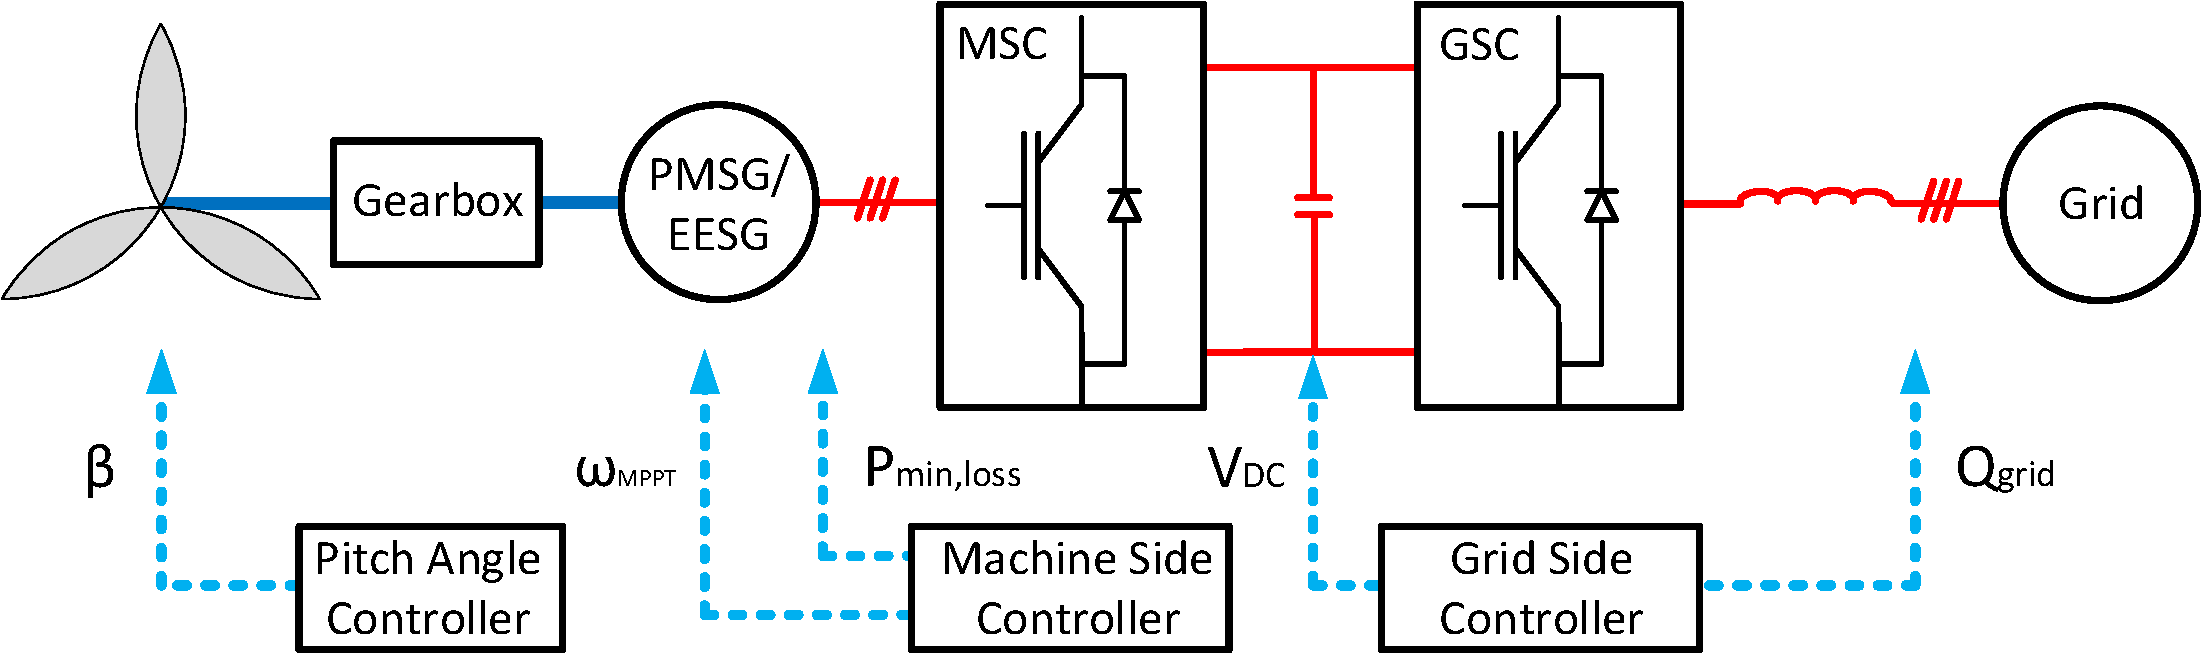
\includegraphics[width=0.9\linewidth]{windmodel2_1.pdf}
		\caption{Geared PMSG/EESG Wind Turbine}		
		\label{varspeedpmsg_1}
	\end{subfigure}
	\vspace{0.1em} % here you can insert horizontal or vertical space
	\begin{subfigure}{0.9\textwidth}
		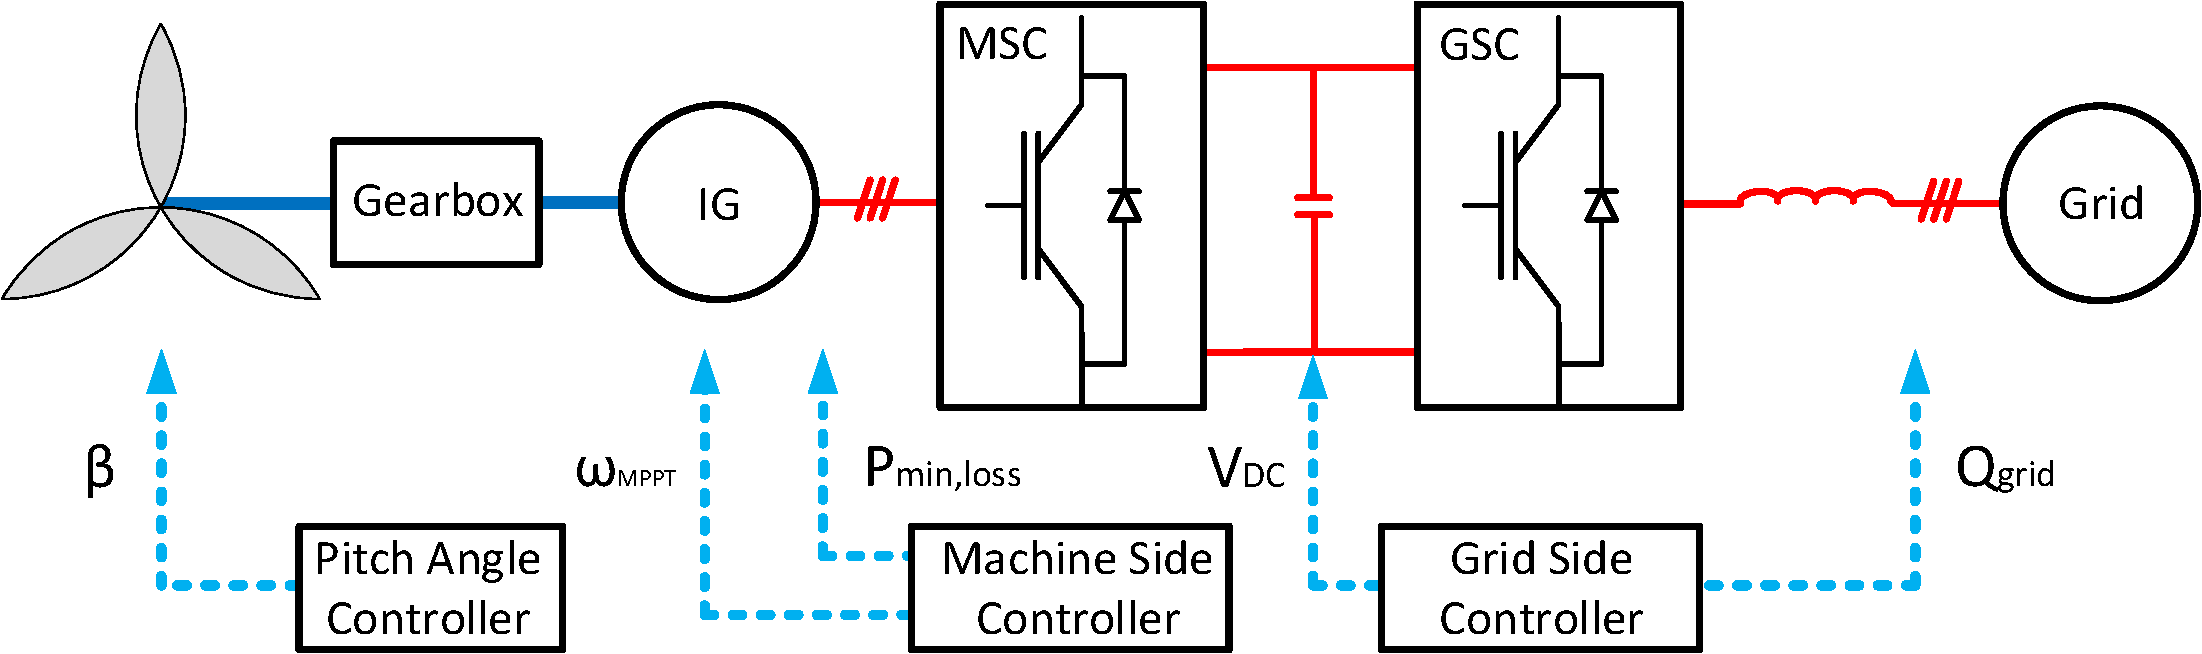
\includegraphics[width=0.9\linewidth]{windmodel2_2.pdf}
		\caption{Geared IG Wind Turbine}
		\label{varspeedpmsg_2}	
	\end{subfigure}
	\vspace{0.1em} % here you can insert horizontal or vertical space
	\begin{subfigure}{0.9\textwidth}
	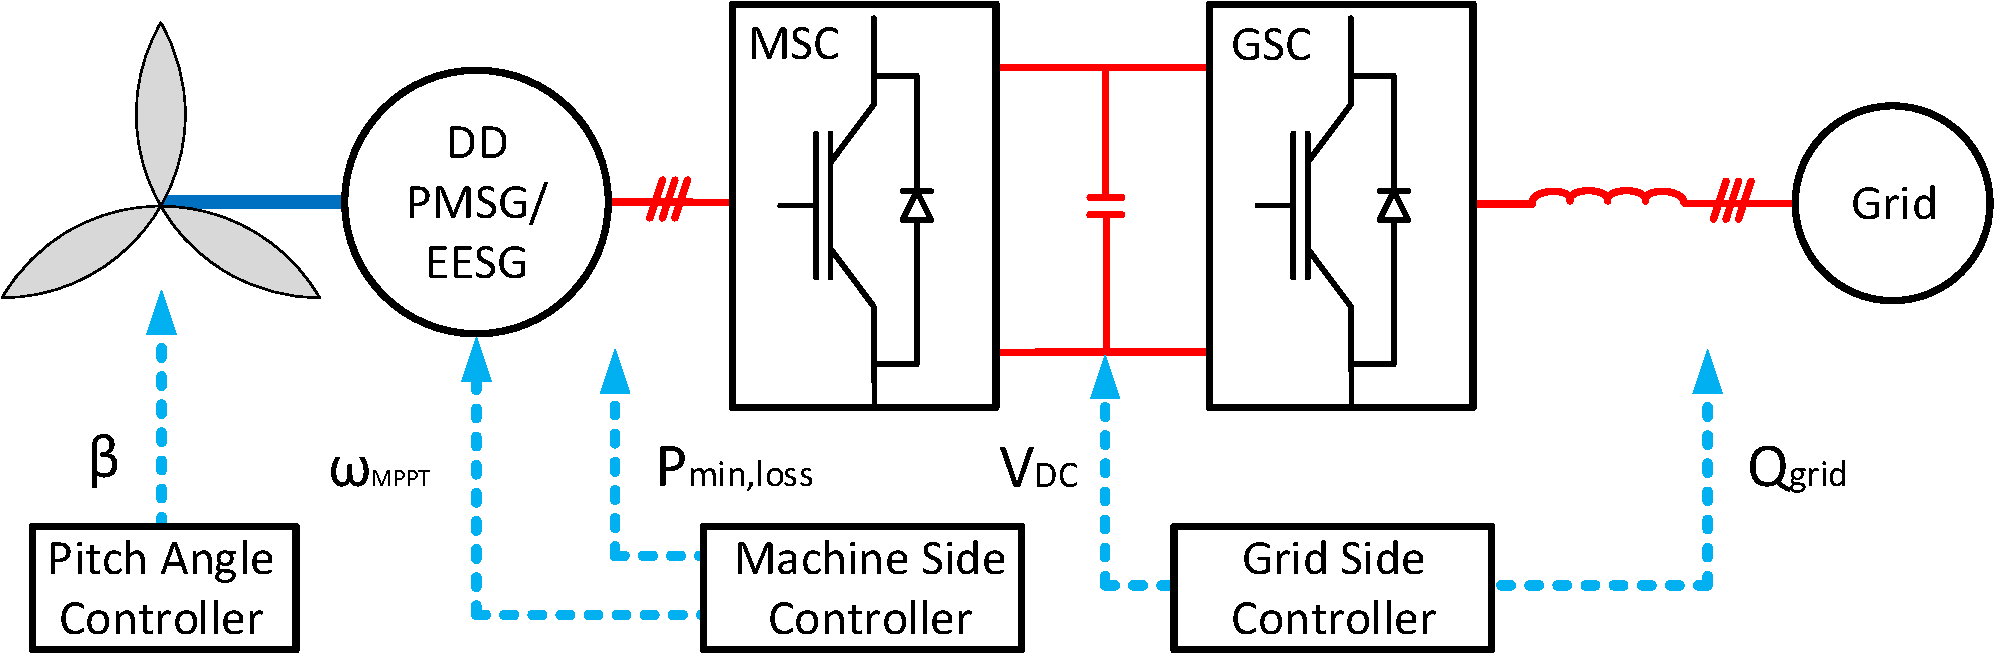
\includegraphics[width=0.9\linewidth]{windmodel2_3.pdf}
	\caption{Direct-Drive PMSG/EESG Wind Turbine}
	\label{varspeedpmsg_3}	
	\end{subfigure}
	\caption{Wind Turbine Topologies with Full-Scale Power Electronics}
\end{figure}
\subsection{Aerodynamic Model}
Aerodynamic model is the sub-model that captures power from the wind. The output of this block is the aerodynamic torque that rotates the turbine. However, the wind speed is not the only input. Turbine speed and pitch angle are also the inputs of the system since they affect the mechanical power that is captured from the wind.\par
The aerodynamic power of wind is given in Eq. (\ref{windpower}) where $\rho_{air}$ is air density in $kg/m^{3}$, $R$ is the blade radius in $m$ abd $v_{wind}$ is the wind speed in $m/s$. Note that this is the available power of the air that is striking the turbine swept area and it is not possible to extract that amount of energy. Otherwise, the air would be standstill behind the wind turbine \cite{Ackermann2005a}.
\begin{equation}
P_{wind}=0.5\rho_{air}\pi R^{2} v_{wind}^{3}
\label{windpower}
\end{equation}
The wind turbine captures a fraction of the available wind power that is denominated as power coefficient $C_{p}$. Therefore, turbine power captured from wind can be found with the Eq. (\ref{turbinepower}).
\begin{equation}
P_{tur}=C_{p}P_{wind}
\label{turbinepower}
\end{equation}
Power coefficient determines the amount of power to be captured from wind and it is a non-linear function of the tip speed ratio, $\lambda$ and pitch angle, $\beta$. Tip speed ratio is a parameter proportional with turbine speed. It can be defined as the ratio of the speed in the turbine tip to the wind speed as in the Eq. (\ref{tipspeed}). Power coefficient for a specific tip speed ratio and pitch angle can be found with the Eq. (\ref{cp}) and (\ref{lambdai}) where $c_{1}$ is 0.5176, $c_{2}$ is 116, $c_{3}$ is 0.4, $c_{4}$ is 5, $c_{5}$ is 21 and $c_{6}$ is 0.0068 \cite{Heier}.\par
\begin{equation}
\lambda=\frac{\omega_{tur}R}{v_{wind}}
\label{tipspeed}
\end{equation}
\begin{equation}
C_{p}(\lambda,\beta)=c_{1}(c_{2}/\lambda_{i}-c_{3}\beta-c_{4})e^{-c_{5}/\lambda{i}}+c_{6}\lambda
\label{cp}
\end{equation}
\begin{equation}
\frac{1}{\lambda_{i}}=\frac{1}{\lambda+0.08\beta}-\frac{0.035}{\beta^{3}+1} 
\label{lambdai}
\end{equation}
\begin{figure}[h!]
	\centering
	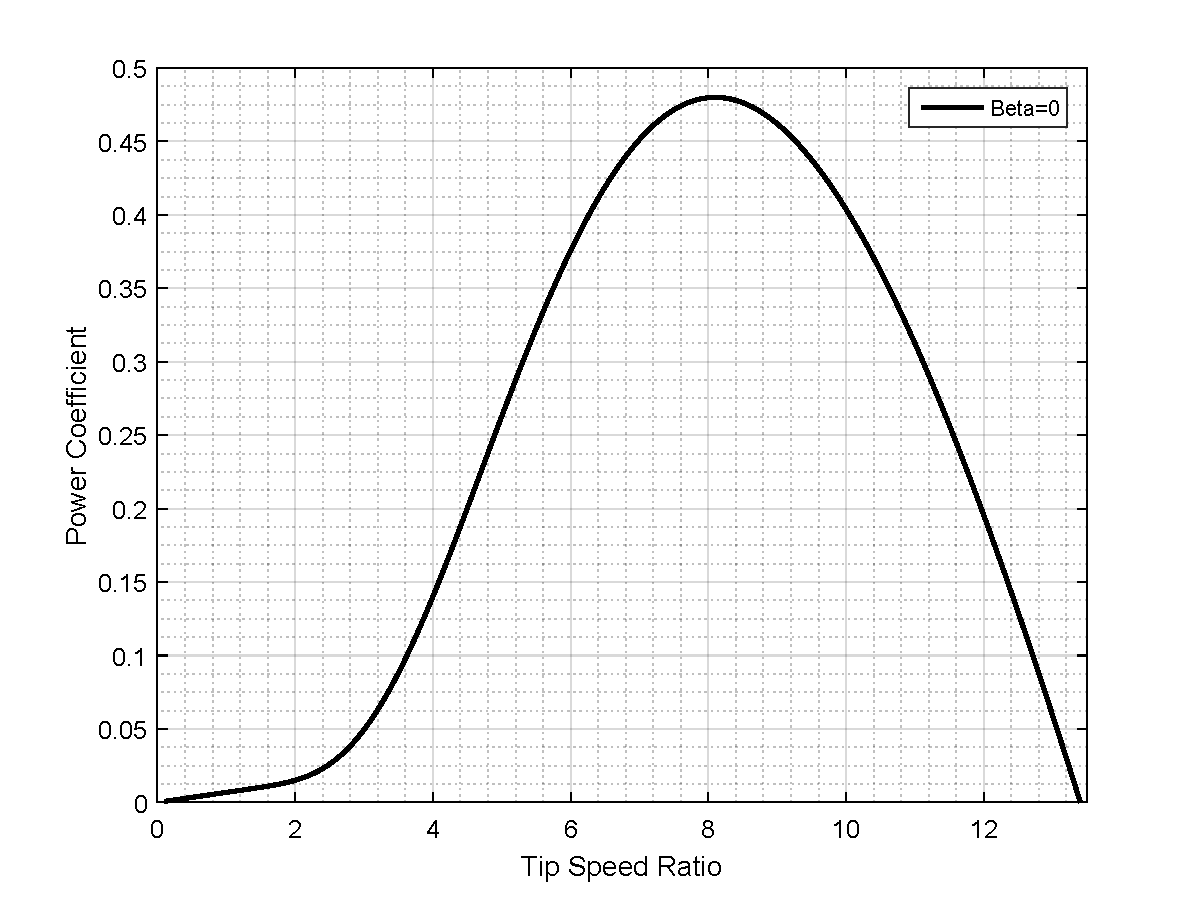
\includegraphics[width=.95\linewidth]{PowerCoefficient.pdf}
	\caption{Power Coefficient Variation with Tip Speed Ratio under Zero Pitch Angle}
	\label{variationofcp}
\end{figure} 
\par
Variation of power coefficient $C_{p}$ is given in Fig. \ref{variationofcp} for varying tip speed ratio. For the zero pitch angle, power coefficient has the maximum value of 0.48 for the tip speed ratio of 8.1. In order to ensure that the maximum of wind power is extracted, wind turbine should rotate a speed that gives the optimum tip speed ratio. This is ensured by the Maximum Power Point Tracking (MPPT) algorithms. 
\subsubsection{Maximum Power Point Tracking Algorithms}
In the literature, different methods are presented in order to operate in the Maximum Power Point. Perturb\&Obserb (P\&O) is the most common MPPT method in the literature \cite{Wang2004}, \cite{Barakati2009}. The methods simply creates a perturbation in the generator speed. The change in the generator speed creates also change in the active power output. If the power is increased with this perturbation, the generator speed is again perturbed in the same direction until a decrease in the active power is observed. This methods is the simplest method and does not require any calculation or wind speed measurement. However, the algorithm creates oscillations in the generator speed and active power. This method is also called as Hill-Climb Search (HCS) method in the literature.\par
Another MPPT algorithm is the wind speed measurement method \cite{Thriringer1993}, \cite{C.A.2013}. If the wind speed is estimated accurately, the optimal generator speed can be calculated. However, wind speed estimation is complicated and increases the cost. Another commonly used MPPT algorithm is the power-signal feedback (PSF) control \cite{C.A.2013},\cite{Wang2004}, \cite{Lu2002}. This method requires maximum power curve of the wind turbine based on the experimental results. A look-up table is constructed with obtained wind turbine speed and active output power values. However, using generator speed and active power measurements is the main drawback of this algorithm. Finally, there are numerous number of much complex MPPT algorithms based on fuzzy-logic \cite{Zeng2008} or neural-network \cite{Lin2011}. However, these MPPT algorithms are out of scope of this thesis. Therefore, optimal generator speed is provided in this study according to the wind speed. 
\subsubsection{Pitch Angle Control}
According to Eq. (\ref{windpower}), wind power increases with the cube of the wind speed. Hence, wind power increases dramatically for the high wind speeds. In order to decrease power, pitch angle i.e. blade angle is increased. Since the power coefficient, $C_{p}$ is a function of the pitch angle, $\beta$, wind power can be curtailed with increased blade angle. Variation of power coefficient for two different pitch angle is shown in Fig. \ref{cpwithtwopitchangle}. Increasing pitch angle by $1.176^{\circ}$ decreases power coefficient by 10\%.\par
\begin{figure}[h!]
	\centering
	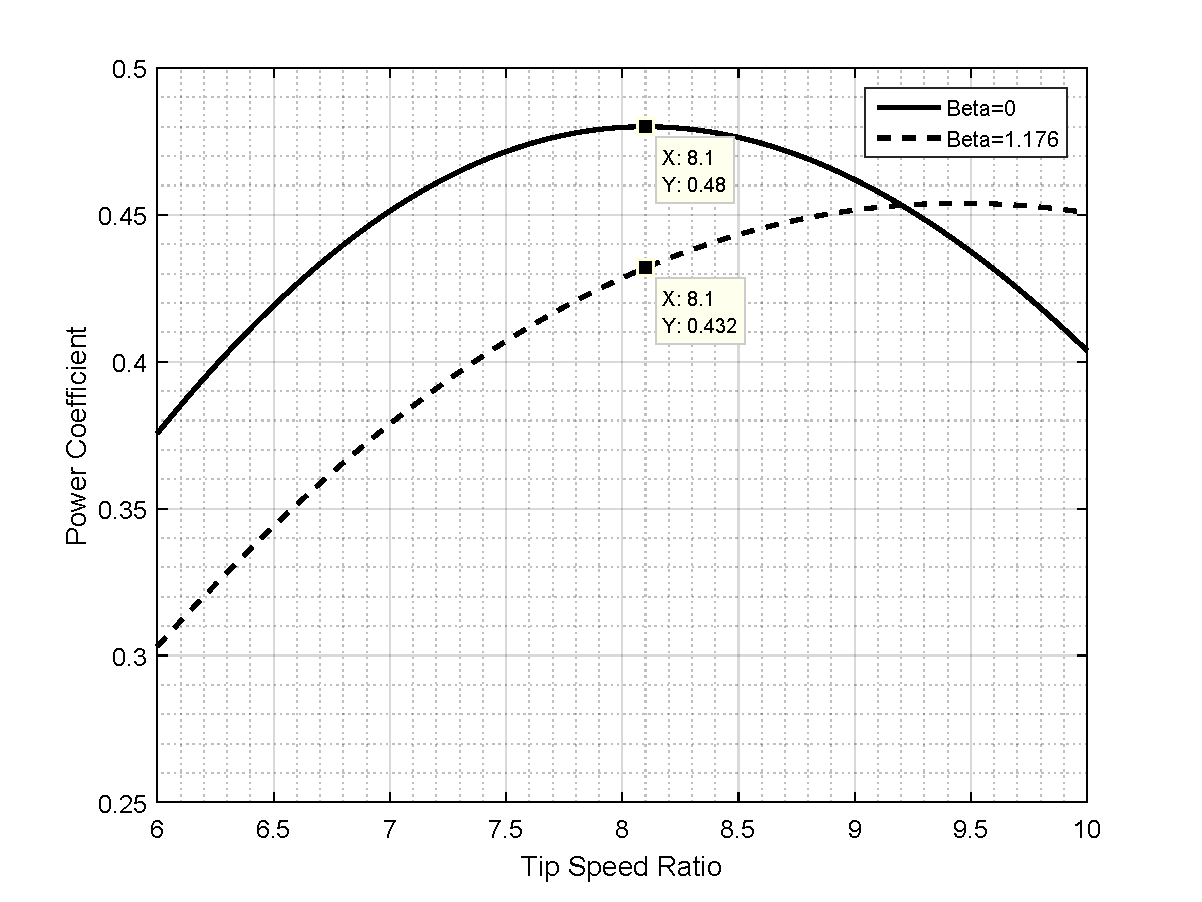
\includegraphics[width=.95\linewidth]{powercoefficient_with_varying_pitch.pdf}
	\caption{Power Coefficient Variation for Two Different Pitch Angle}
	\label{cpwithtwopitchangle}
\end{figure} 
As long as wind power is below the rated power, the wind turbine is operated in MPPT speed. This is ensured by obtaining optimal tip speed ratio. This means that for zero pitch angle, MPPT speed is increased linearly with wind speed. Before reaching rated power, MPPT speed might reach maximum generator speed. In this case, wind turbine reference speed will be the maximum generator speed. However, turbine speed cannot be decreased down to reference speed when the torque limit is reached. Hence, the pitch angle should be increased to regulate the turbine speed. Pitch angle controller is depicted in Fig. \ref{pitchcontroller}. Notice that the pitch angle is increased when the speed exceeds maximum generator speed. Otherwise, the pitch angle kept as zero.\par
\begin{figure}[h]
	\centering
	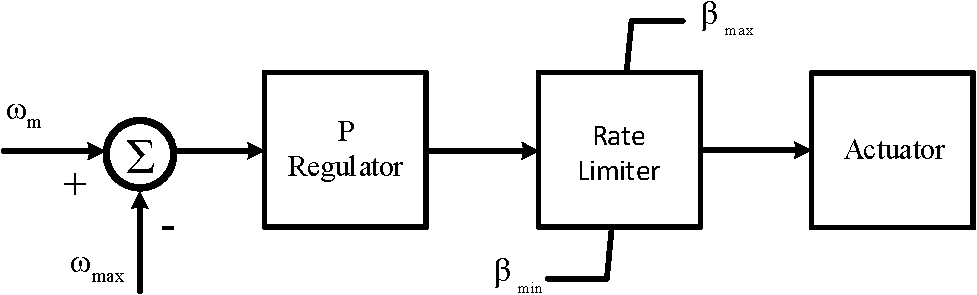
\includegraphics[width=.8\linewidth]{pitchcontroller2.pdf}
	\caption{Pitch Angle Control Diagram}
	\label{pitchcontroller}
\end{figure}
The responsibility of the pitch angle controller is the regulation of the blade angle but each blade in the wind turbine is a few tonnes. Therefore, the blade angle cannot be changed instantaneously and limited with rate limiter. The rate of change of pitch angle in this study is limited with $10^{\circ}/s$ \cite{Ackermann2005a}. Besides, the pitch angle controller takes action as soon as the maximum generator speed is exceeded. Therefore, wind turbine operation deviates from optimal tip speed ratio. This can also be observed from the variation of power coefficient, $C_{p}$ with the wind speed for the wind turbine GE 2.75-103 used in this study. Variation of the $C_{p}$ is shown in Fig. \ref{powercoefficientge}.
\begin{figure}[h!]
	\centering
	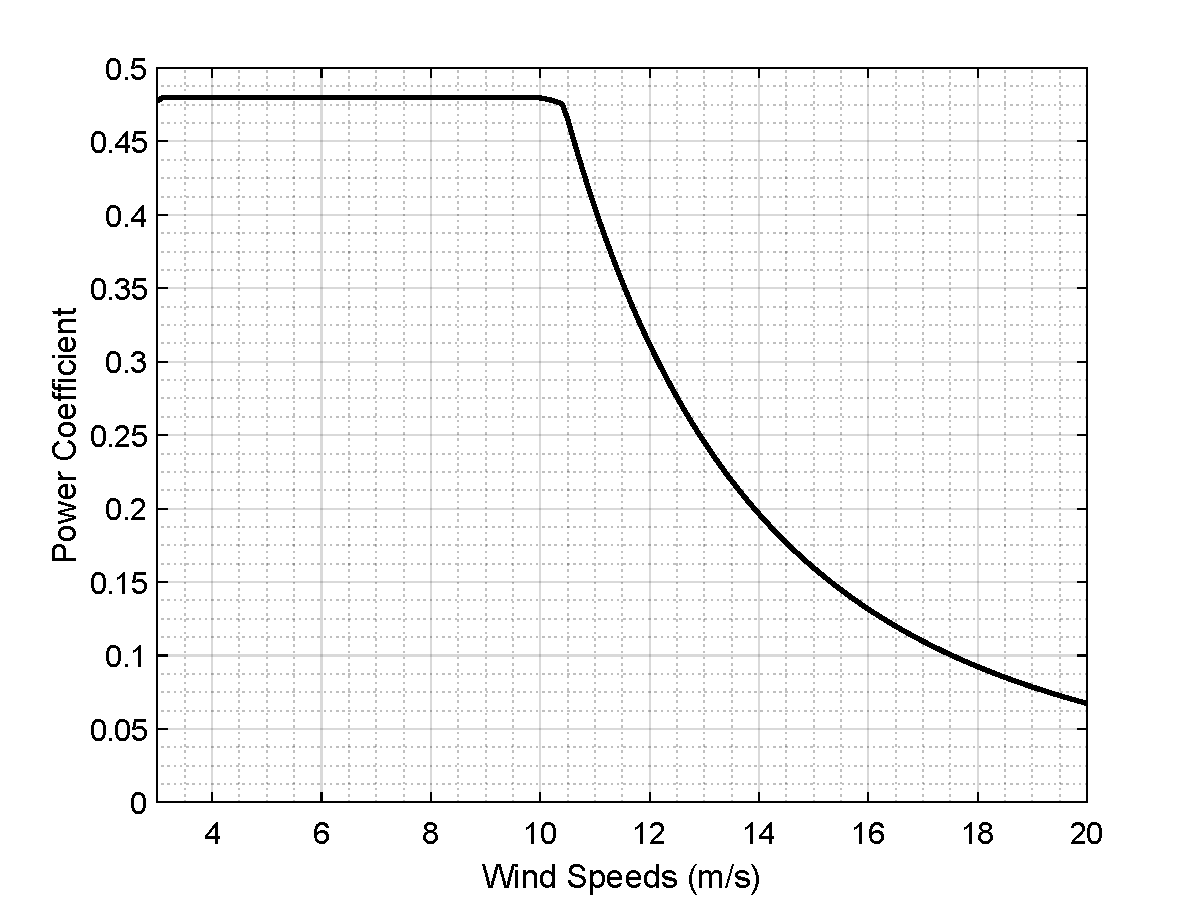
\includegraphics[width=.9\linewidth]{cp_wind.pdf}
	\caption{Power Coefficient Variation for GE 2.75-103}
	\label{powercoefficientge}
\end{figure}
\subsection{Gearbox}  
Variable speed PMSG wind turbines have a gearbox between turbine and generator except for direct-drive wind turbines. The gearbox increases angular speed and decreases the torque in the generator side. By decreasing the rated torque, generator size and cost can be reduced since the generator size is almost proportional to rated torque due to constant shear stress \cite{Polinder2013aa}. Moreover, turbine speed is increased to the allowable speed range of the generator which is generally much higher than that of wind turbines. Otherwise, generator should have high pole numbers. \par
A gearbox model is depicted in Fig. \ref{gearboxmodel}. They are mainly used for speed and torque conversion. It should be noted that the gearboxes are lossy systems. Therefore, the output torque of the gearbox would be lower than the ratio of input torque to gearbox conversion ratio. Direct-drive systems are based on the elimination of the gearbox systems by direct connection between turbine and generator in order to increase efficiency and reliability \cite{Chen2009b}. In this study, 3 stage (1 planetary / 1 helical) gearbox is modelled with \%97 efficiency \cite{UKONSAARI2016}. 
\begin{figure}[h!]
	\centering
	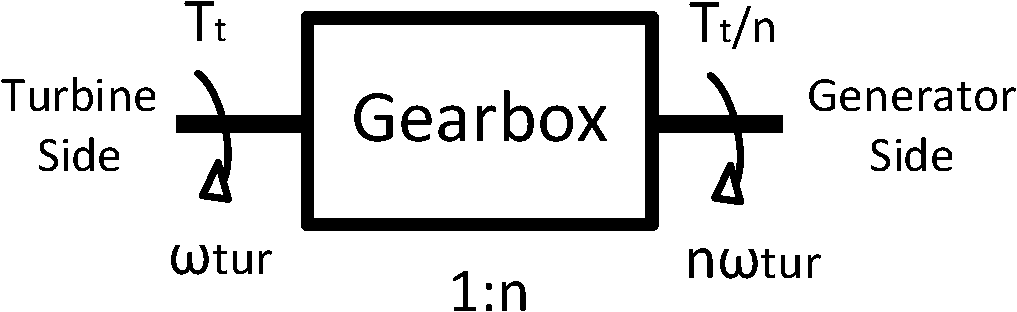
\includegraphics[width=.5\linewidth]{gearbox.pdf}
	\caption{Gearbox Modelling}
	\label{gearboxmodel}
\end{figure}
\subsection{Permanent Magnet Synchronous Generator}
\label{pmsgsection}
PMSGs and electrically excited generators can be employed with full-scale power electronics. However, PMSGs are generally preferred over electrically excited synchronous generators due to their high efficiency. The absence of electrical excitation on the rotor decreases losses. Besides, slip ring is not needed in the generator which also increases the reliability of the PMSG wind turbines. Dynamical equations of the salient pole PMSG are projected on a reference frame which rotates synchronously with magnet flux and given in Eq. (\ref{v1d}) and (\ref{v1q}) where $R_{1}$ is stator resistance in $\Omega$, $L_{sd}$ and $L_{sq}$ are d and q axis inductances in $H$, $i_{ad}$ and $i_{aq}$ are d and q axis currents in $A$, $\omega$ is the electrical angular frequency in $rad/s$, $\psi_{f}$ is magnet flux linkage in $Vs$ \cite{Ackermann2005a}. 
\begin{equation}
v_{1d}=R_{1} i_{ad}+L_{sd}\frac{di_{ad}}{dt}-L_{sq}\omega i_{sq}
\label{v1d}
\end{equation}
\begin{equation}
v_{1q}=R_{1} i_{aq}+L_{sq}\frac{di_{aq}}{dt}+L_{sd}\omega i_{sd}+\omega \psi_{f}
\label{v1q}
\end{equation}
Another important PMSG parameter is the power in dq frame. The power expression is given in Eq. (\ref{pmsgpower}). The electromechanical torque can be found by the relation between power and angular speed. The torque expression is also given in Eq. (\ref{pmsgtorque}) where p is the number of pole pair.
\begin{equation}
P_{elm}=\frac{3}{2}\omega i_{aq} (\psi_{f}+i_{ad}(L_{sq}-L_{sd}))
\label{pmsgpower}
\end{equation}
\begin{equation}
T_{e}=\frac{P_{elm}}{w_{m}}=\frac{P_{elm}}{w/p_{p}}=\frac{3}{2}p_{p} i_{aq} (\psi_{f}+i_{ad}(L_{sq}-L_{sd}))
\label{pmsgtorque}
\end{equation}

Given equations are defined for salient pole machines. If the clyndrical rotor machine is used, the torque equation reduces to the Equation \ref{pmsgtorque2}.
\begin{equation}
T_{e}=\frac{3}{2}p_{p} i_{aq} \psi_{f}
\label{pmsgtorque2}
\end{equation}
\subsection{Machine Side Converter}
Variable speed wind turbines that are equipped with the back-to-back converters are able to decouple grid frequency and the turbine speed. This gives wind turbine degree of freedom for the rotational speed. In this way, turbine is able to capture the maximum available power from wind. Machine Side Converter (MSC) i.e. Generator Side Converter is the converter that is connected between generator and DC-bus. The three phase generator output AC voltage is converted to DC voltage. Conversion from AC to DC can be achieved by three-leg full bridge converters. This converter can be equipped with uncontrolled, semi-controlled and fully-controlled switches. Fully-controlled switches such as MOSFET,IGBT are commonly used in the industry and gives two control parameters to the user. \par
Voltages and currents are generally transformed into synchronously rotating reference frame or also called dq frame. Since the frame is rotating in synchronous speed, three-phase phasors are transformed to DC quantities. Therefore, its control becomes easier \cite{Kazmierkowski2002}. Proportional-integral (PI) controllers are associated with the dq control structure due to their satisfactory behaviour interaction to DC variables \cite{Blaabjerg2006a}. Hence, the control in the back-to-back converter is achieved with PI controllers in the dq frame. \par
\begin{figure}[h!]
	\centering
	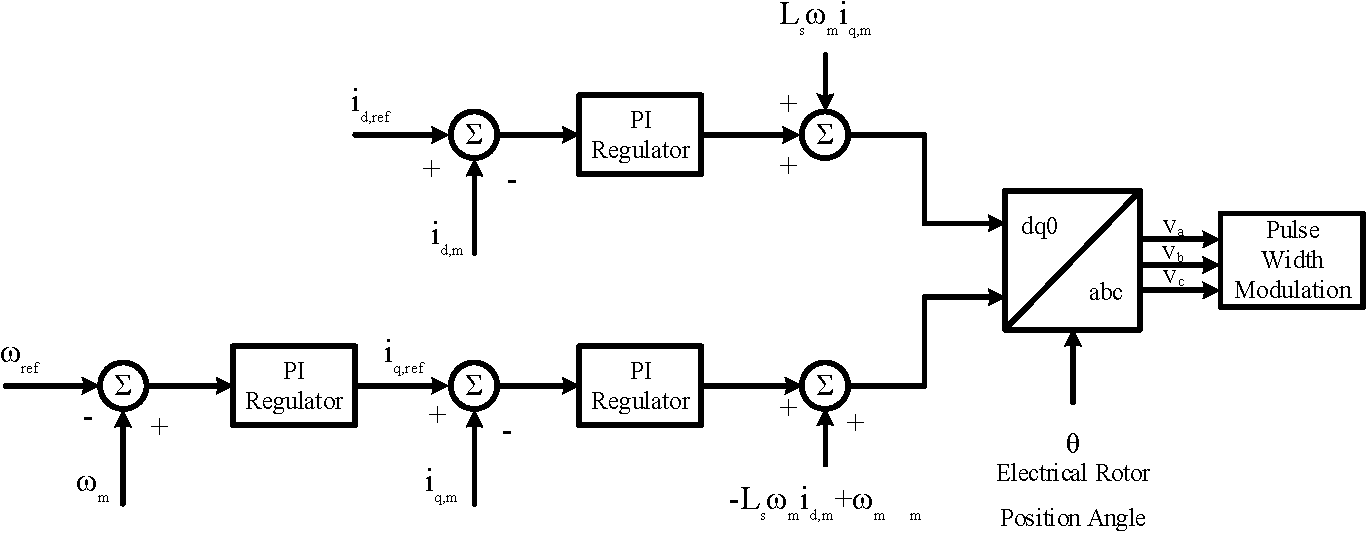
\includegraphics[width=.95\linewidth]{msc.pdf}
	\caption{Machine Side Controller Diagram}
	\label{msc}
\end{figure}
The control diagram of the MSC is depicted in Fig. \ref{msc} according to the study in \cite{Chinchilla2006}. In dq frame, it is possible to control two parameters. One of these parameters is the d-axis current that is set zero in order to decrease the stator copper losses. The other parameter is the q-axis current that is proportional to the electromagnetic torque as it can be observed in the Eq. (\ref{pmsgtorque2}). However, q-axis current or torque is controlled in order to regulate the turbine speed. Therefore, turbine speed is adjusted such that the turbine will capture maximum available power in the wind. 
\subsection{Grid Side Converter}
Grid Side Converter (GSC) or Line Side Converter (LSC) is the converter that is connected between DC-link capacitor and grid. GSC works as an inverter that injects current synchronous to grid. Currents and voltages are transformed into synchronously rotating frame that is aligned with the grid voltage. Therefore, d-axis current determines the amount of current which is in phase with the grid voltage meanwhile q-axis current determines amount of current that is out of phase with the grid voltage. In other words, injecting d-axis current injects active power to grid meantime q-axis current injects reactive power to grid.\par
The responsibility of the GSC is regulating DC voltage and the reactive power injected to the grid. The control diagram of the GSC is given in Fig. \ref{gsc}. As seen from the figure, DC-bus voltage is regulated by controlling the d axis current. If the DC-bus voltage increases above the reference value, d-axis current reference is increased. As a result, active power increases. Increased active power also decreases the DC-bus voltage level. Reference value of the q-axis current is set to zero in normal operation, consequently unity power factor. For Low Voltage Ride-Through studies, q-axis current is determined according to the reactive power value requirement. \cite{Orowska-Kowalska2014} \par
\begin{figure}[h!]
	\centering
	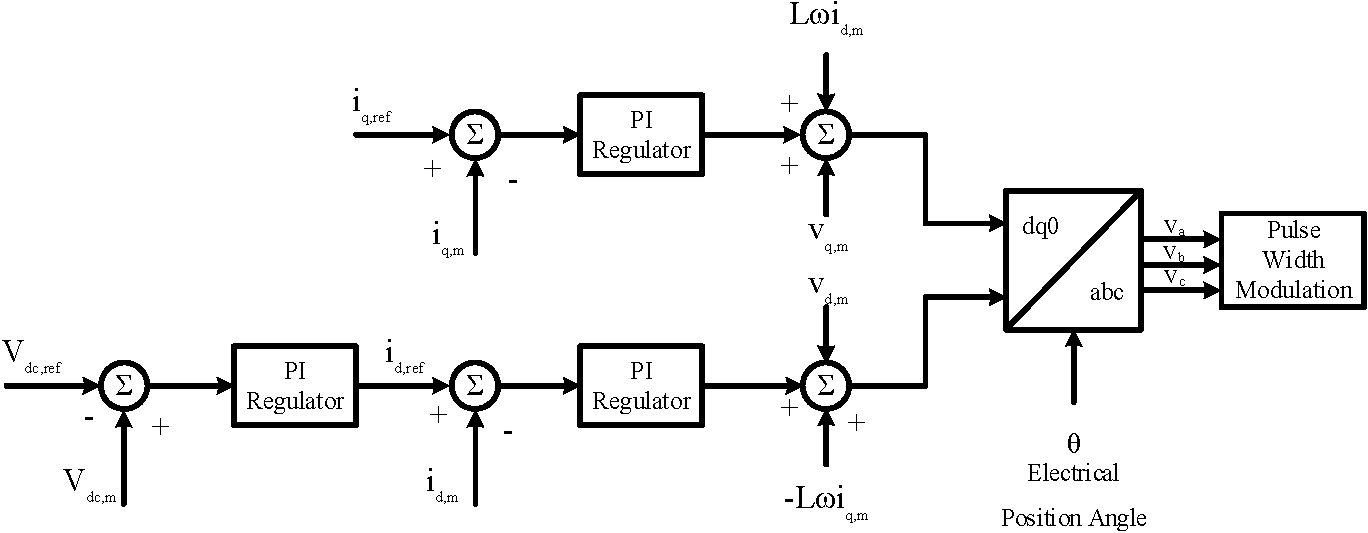
\includegraphics[width=.98\linewidth]{gsc.pdf}
	\caption{Grid Side Controller Diagram}
	\label{gsc}
\end{figure}
GSC is connected to grid through a filter. Therefore, the output voltage of the converter is not equal to the that of grid. The relation between converter voltage, grid voltage and current is derived through Eq. (\ref{crossilk}) to (\ref{crosscomp2}) where $v_{c}$ is the converter voltage, $v_{g}$ is the grid voltage and  $i_{g}$ is the grid current measured in the grid side. As it is observed in Eq (\ref{crosscomp1}) and (\ref{crosscomp2}), converter side voltage includes same axis grid voltage and a term proportional to cross axis current which is called cross-coupled term. Therefore, the outputs of the inner PI regulators are compensated and forwarded to Pulse Width Modulation after transformation to three-phase voltages.
\begin{equation}
\overline{v_{c}}=v_{dc}+jv_{qc}
\label{crossilk}
\end{equation}
\begin{equation}
\overline{v_{g}}=v_{dg}+jv_{qg}
\end{equation}
\begin{equation}
\overline{i_{g}}=i_{dg}+ji_{qg}
\end{equation}
\begin{equation}
\overline{v_{c}}=\overline{v_{g}}+\overline{i_{g}}j\omega L
\end{equation}
\begin{equation}
v_{dc}+jv_{qc}=v_{dg}+jv_{qg}+j\omega L (i_{dg}+ji_{qg})
\end{equation}
\begin{equation}
v_{dc}=v_{dg}-\omega L i_{qg}
\label{crosscomp1}
\end{equation}
\begin{equation}
v_{qc}=v_{qg}+\omega L i_{dg}
\label{crosscomp2}
\end{equation}
The PI regulators of the wind turbine model is tuned with trial error method. In this study, the modelled wind turbine is connected to grid with an L filter even though the actual turbine is connected to grid with an LCL filter. However, the actual system would operate better than the modelled case since the the LCL filter has superior performance than L filters \cite{Brantsater2015}. Nonetheless, L filter has provided sufficient performance for the successful operation of the wind turbine in this study regardless from the power quality standards in the output current. The active power of the wind turbine under varying wind speed is given in the Fig. \ref{powerdata}. \par
\begin{figure}[h!]
	\centering
	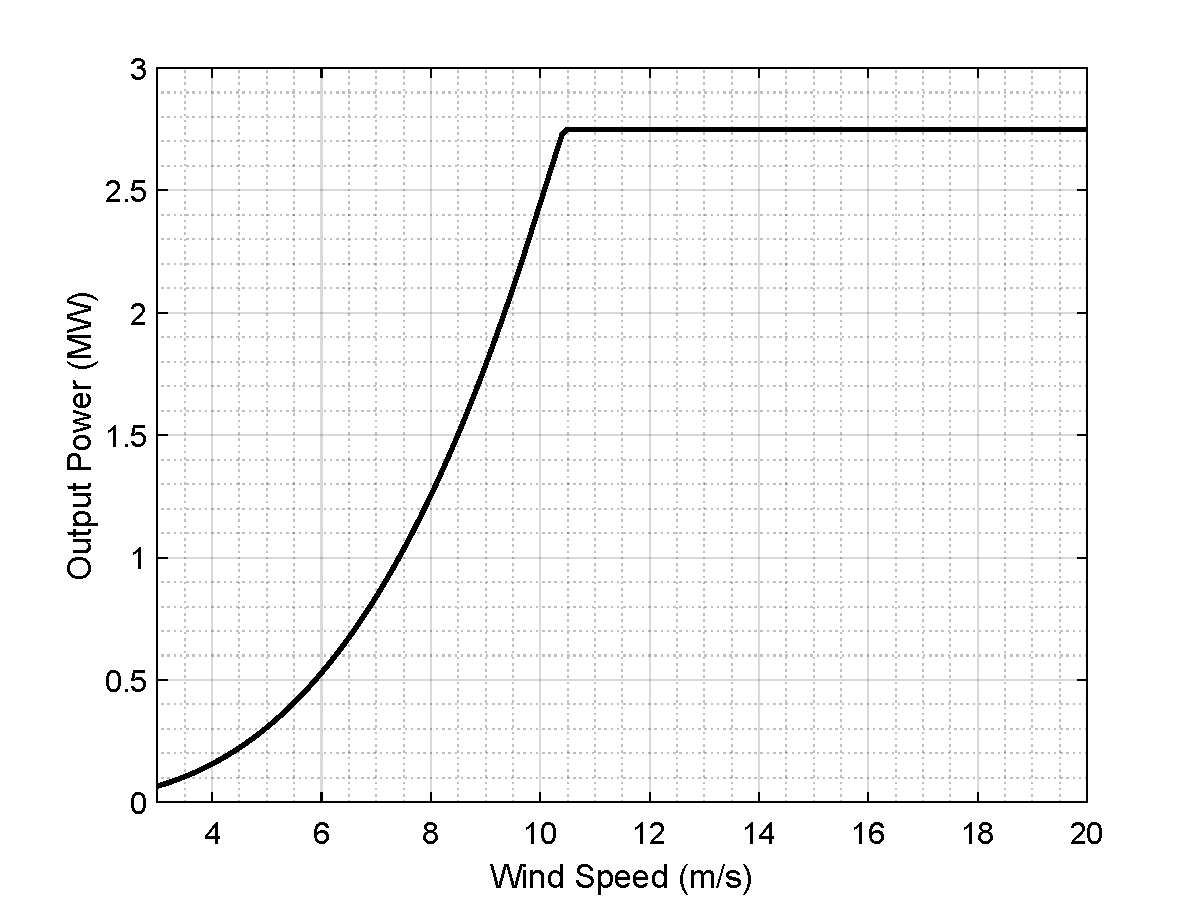
\includegraphics[width=.9\linewidth]{powerdata.pdf}
	\caption{Variation of the Active Power of the Wind Turbine}
	\label{powerdata}
\end{figure}
\section{Synthetic Inertia Implementation}
As explained Section \ref{swing}, synchronous generators change their speed according to the balance between input mechanical and electromechanical powers. Furthermore, if the frequency changes, the electromechanical power of the generators also change. Nonetheless, the renewable energy systems which are connected to grid with a power electronics interface are unresponsive to the deviations in the grid frequency.\par
The definition of the synthetic inertia is the controlled contribution of electrical torque that is proportional to RoCoF in the unit connection terminal \cite{Eriksson2017}. Synthetic inertia (also called as 'virtual inertia') is the method that emulates the synchronous generator in the renewable energy systems. In this method, the active power output of the wind turbines are adjusted according to the Eq. (\ref{synthetic}) where $H_{syn}$ is the synthetic inertia constant in seconds and $\omega_{t}$ is the terminal angular frequency in pu. The increase in the active power is proportional to RoCoF as well as the emulated inertia constant. The emulated inertia constant can be different from the inertia constant of the renewable energy system. For instance, the solar PV systems does not have inertia. Even in these systems, an inertia constant can be emulated as long as the system includes stored energy. In the wind turbines, the additional energy can be yielded from the kinetic energy in the turbine inertia. For solar PV systems, energy storage systems or the store energy in the DC-link capacitor can be utilized.\par
\begin{equation}
\Delta P_{e}=-2H_{syn}\frac{d\omega_{t}}{dt}\omega_{t}
\label{synthetic}
\end{equation}
In order to implement synthetic inertia in the system, a relation between frequency and active power of the wind turbine should be constructed. Wind turbine in this study is variable speed wind turbine with full scale power electronics. The speed of the turbine is controlled by MSC such that active power is adjusted. Inertial support modification is depicted in Fig. \ref{modifiedmsc}. The new value of the active power is determined according to the swing equation. However, the wind turbine in this study is operated with a reference speed rather than a reference power. Therefore, the assigned power value should be used in order to yield the q-axis current reference value. Reference q-axis current is derived between the Eq. (\ref{inertialsupport1}) to Eq. (\ref{inertialsupport4}).\par
\begin{figure}[h!]
	\centering
	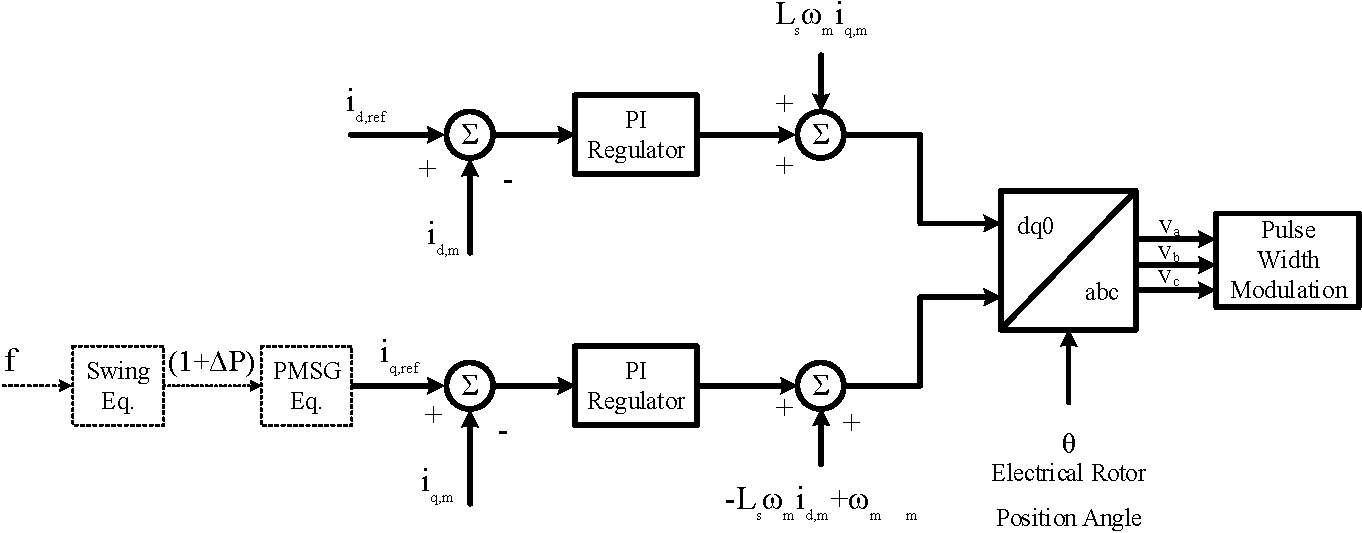
\includegraphics[width=.98\linewidth]{msc_modified.pdf}
	\caption{Modified MSC for Inertial Support}
	\label{modifiedmsc}
\end{figure}
\begin{equation}
P_{new}=(1+\Delta P) P_{pre}
\label{inertialsupport1}
\end{equation}
\begin{equation}
T_{new} \omega_{m}=(1+\Delta P) T_{pre} \omega_{pre}
\label{inertialsupport2}
\end{equation}
\begin{equation}
\frac{3}{2} p_{p} \psi_{f} i_{q,new} \omega_{m}=(1+\Delta P) \frac{3}{2} p_{p} \psi_{f} i_{q,pre} \omega_{pre}
\label{inertialsupport3}
\end{equation}
\begin{equation}
 i_{q,ref}=i_{q,new}=(1+\Delta P) \frac{i_{q,pre} \omega_{pre}}{ \omega_{m}} 
\label{inertialsupport4}
\end{equation}
\subsection{Synthetic Inertia Activation Schemes}
Another issue about inertial support is the time instant to trigger synthetic inertia. In the literature, continuous operation, under-frequency trigger and maximum-frequency gradient are discussed \cite{Gonzalez-longatt2015}. It is obvious that continuous operation would create oscillations in active power output due to the continuous deviations in grid frequency. This is an unrealistic operation and is used for comparison purposes.\par
Second activation method is the under-frequency trigger which is the activation when the frequency decreases below a threshold value. It can be used for capturing the time instant for the inertial support. However, power grid might be in a stable point even if the frequency is 49.8Hz. Therefore, this method would be unsuccessful depending on the disturbance event. \par 
Third activation scheme is the maximum-frequency gradient trigger. It uses a controller that is very similar to RoCoF relays and tracks the frequency gradient. Once the frequency gradient is below a threshold value, the synthetic inertia is activated. Since the severity of frequency disturbance event is related to the RoCoF, this activation scheme is the most remarkable scheme \cite{Gonzalez-longatt2015}. \par The activation of the inertial support by only frequency-gradient (RoCoF) might be misleading. For instance, a negative RoCoF value when the frequency is above the nominal value is not a frequency disturbance. Therefore, the inertial support should not be activated unless the frequency is below a threshold. Thus, in this study, maximum-frequency gradient is used in coordination with the under-frequency trigger. \par 
Grid RoCoF changes in the grid according to the disturbance level as well as the grid inertia. According to the disturbances in the Continental Europe System within the last 15 years, RoCoFs in the range between 0.1Hz/s and 1Hz/s are observed \cite{ENTSO-E2016}.Therefore in this study, 0.1Hz/s of RoCoF threshold with a frequency dead-band of 10mHz is selected. In this way, a negative RoCoF above 49.99Hz is not captured as events as long as it does not decrease below the under frequency threshold.
\subsection{Source of the Inertial Support}
The renewable energy systems cannot determine the amount of power in contrast the conventional systems. A thermal power plant, for instance, adjusts its power output as desired. However, the source of power in renewable energy is intermittent due to nature of the power source. This is why a spare energy is required in order to change the power output.\par
The stored energy in a wind turbine exists in the generator and turbine inertia. Therefore, the drive train of the wind turbine is important for the stored energy in the turbine. Different drive train concepts are compared in Table \ref{gencompare} according to the typical generator data presented in \cite{Seman2011}. According to the typical generator data and typical gearbox ratios, the stored energy with the High Speed Full Converter (HSFC) is calculated as 16.2MJ meanwhile DFIG concept stored 15.7MJ. However, the Direct-Drive concept stores 13.6MJ energy. Even though the stored energies close to each other, it is observed that the higher speed generator concepts store more than that of lower speed concepts. Notice that the wind turbine studied in thesis is a 3 stage HSFC wind turbine which store the highest energy compared to the other drive trains in the same power class.
% Please add the following required packages to your document preamble:
% \usepackage{graphicx}
\begin{table}[h!]
	\centering
	\resizebox{\textwidth}{!}{%
		\begin{tabular}{|c|c|c|c|c|}
			\hline
			\textbf{\begin{tabular}[c]{@{}c@{}}Drive\\   Train Concept\end{tabular}}       & \begin{tabular}[c]{@{}c@{}}Doubly-Fed \\ 3 Stage Gear\end{tabular} & \begin{tabular}[c]{@{}c@{}}Low Speed\\ Full Converter \\ (LSFC)\\   Direct Drive\end{tabular} & \begin{tabular}[c]{@{}c@{}}Medium Speed\\ Full Converter\\   (MSFC) \\ 2 Stage Gear\end{tabular} & \begin{tabular}[c]{@{}c@{}}High Speed\\ Full Converter\\  (HSFC)\\ 3 Stage Gear\end{tabular} \\ \hline
			\textbf{Generator Type}                                                        & DFIG                                                               & PMSG                                                                                          & PMSG                                                                                             & PMSG                                                                                         \\ \hline
			\textbf{\begin{tabular}[c]{@{}c@{}}Generator\\ Inertia \\ (kgm2)\end{tabular}} & 250                                                                & 40500                                                                                         & 510                                                                                              & 115                                                                                          \\ \hline
			\textbf{\begin{tabular}[c]{@{}c@{}}Generator Speed\\   (rpm)\end{tabular}}     & 1200                                                               & 14                                                                                            & 400                                                                                              & 1600                                                                                         \\ \hline
			\textbf{\begin{tabular}[c]{@{}c@{}}Gearbox\\   Ratio\end{tabular}}             & 85                                                                 & -                                                                                             & 28                                                                                               & 110                                                                                          \\ \hline
			\textbf{\begin{tabular}[c]{@{}c@{}}Blade\\   Inertia\\ (kgm2)\end{tabular}}    & 12600000                                                           & 12600000                                                                                      & 12600000                                                                                         & 12600000                                                                                     \\ \hline
			\textbf{\begin{tabular}[c]{@{}c@{}}Stored\\   Energy (MJ)\end{tabular}}        & 15.7                                                               & 13.6                                                                                          & 14.5                                                                                             & 16.2                                                                                         \\ \hline
		\end{tabular}%
	}
	\caption{Stored Energy Comparison for Different Drive Train Concepts}
	\label{gencompare}
\end{table}
\begin{equation}
E_{electrostatic}=\frac{1}{2} C_{DC}V_{DC}^{2}
\label{electrostatic}
\end{equation}
Energy stored in DC bus capacitor is the only stored energy in PV systems. The amount of energy is given in Eq. (\ref{electrostatic}) and negligible for inertial support studies. In the wind energy systems, there exists significant amount of kinetic energy (above 10MJ) in wind turbine generator and blades in addition to electrostatic energy. The kinetic energy expression is given in Eq. (\ref{kineticenergy}). It should be noted that $J_{total}$ is the equivalent inertia in the generator side as given in Eq. (\ref{totalinertia}),$n$ is the gearbox conversion ratio and $\omega_{m}$ is the speed of the generator.
\begin{equation}
J_{total}=\frac{J_{tur}}{n^{2}} + J_{gen}
\label{totalinertia}
\end{equation}
\begin{equation}
E_{kinetic}=\frac{1}{2} J_{total}\omega_{m}^{2}
\label{kineticenergy}
\end{equation}
Notice that the amount of kinetic energy is dependent on the generator speed. Therefore, the stored energy in wind turbine change according to the generator speed. Moreover, it can also be concluded that the energy is dependent on the wind speed. However, the generator speed is kept constant if the wind speed increases above the rated wind speed. \par
To illustrate the situation better, the electrostatic energy stored in DC bus and kinetic energy in turbine equivalent inertia are compared for GE2.75-103 wind turbine. The wind turbine has a DC bus capacitance of $27mF$ and $1200V$ DC link voltage. The corresponding electrostatic energy is calculated in Eq. (\ref{electrostatic2}). The generator speed of the corresponding generator is between $550rpm$ and $1735rpm$. The total turbine inertia is $1058.2 kgm^2$ in the generator side. The minimum and maximum kinetic energy values are calculated in Eq. (\ref{kineticenergymin}) and (\ref{kineticenergymax}). \par
\begin{equation}
E_{DC-Link}=\frac{1}{2} 27 (10^{-3}) 1200^{2}=19.44kJ
\label{electrostatic2}
\end{equation}
\begin{equation}
E_{kinetic,min}=\frac{1}{2} (1058.2) 57.6^{2}=1755.17kJ
\label{kineticenergymin}
\end{equation}
\begin{equation}
E_{kinetic,max}=\frac{1}{2} (1058.2) 181.7^{2}=17466.02kJ
\label{kineticenergymax}
\end{equation}
It is obvious that the stored kinetic energy in the wind turbine is 90 times of the energy stored in DC bus capacitor even in the minimum generator speed. Therefore, utilization of the kinetic energy for inertial support studies is more efficient than using the stored energy in the capacitor. \par
\begin{table}[h]
	\centering
	\begin{tabular}{ccc}
		\hline
		Parameters                                                           & Minimum & Maximum \\ \hline
		\begin{tabular}[c]{@{}c@{}}Generator Speed\\ (rad/s)\end{tabular}    & 57.6    & 181.7   \\
		\begin{tabular}[c]{@{}c@{}}Stored Kinetic Energy\\ (kJ)\end{tabular} & 1755    & 17466   \\
		\begin{tabular}[c]{@{}c@{}}Inertia Constant\\ (s)\end{tabular}       & 0.58    & 5.75    \\ \hline
	\end{tabular}
	\caption{Dynamic Parameters of the Wind Turbine}
	\label{windpar}
\end{table}
Dynamical parameters of the wind turbine are listed in the Table \ref{windpar}. The stored energy in the turbine equivalent inertia varies with the square of the generator speed. Therefore, the minimum stored energy is one tenth of the maximum case. As a result of this, the inertia constant of the wind turbine is dependent on the wind speed and varies between 0.58s and 5.75s. Notice that the inertia constants to be emulated by wind turbine in this thesis are not restricted to these inertia constant. Wind turbines can emulate higher inertia constants as long as they can increase the output power to desired levels.
\section{Conclusion}
In this chapter, the detailed modelling for PMSG wind turbine is presented. The MSC which is responsible for adjusting the turbine speed for MPPT operation is modified such that the wind turbine provides inertial support. The additional active power is obtained with the kinetic energy extraction from the turbine inertia. \par
The requirement of the inertial support provision is the back-to-back converter that enables the active power and speed control. Therefore, the method described in this chapter is not specific to PMSG wind turbines but the ones with full-scale power electronics. 
% CHAPTER 1
\chapter{INVESTIGATION OF INERTIAL SUPPORT PRACTICAL LIMITS}
\label{chp:4}
\section{Inertial Support Limits}
The source of power in a wind turbine is the aerodynamic wind power, $P_{wind}$ which is constant for a constant wind speed, pitch angle and generator speed. In the steady state, this power is transferred through MSC as $P_{gen}$. If there is a difference between $P_{wind}$ and $P_{gen}$, the difference is either stored in or extracted from the turbine and generator inertia as in the form of kinetic energy. Grid power, $P_{grid}$ is received from MSC and injected grid. The difference between $P_{gen}$ and $P_{grid}$ is stored in or extracted from DC-bus capacitance. The active power flow diagram is depicted in Fig. \ref{power_flow}. As mentioned in Chapter \ref{chp:3}, stored energy exists in turbine and generator inertia and DC-bus capacitance. However, it is also stated that the $E_{kin}$ is much larger than $E_{DC}$ even in the lowest generator speed. Therefore, the source of the inertial support studies is the kinetic energy stored in the inertia. \par
\begin{figure}[h!]
	\centering
	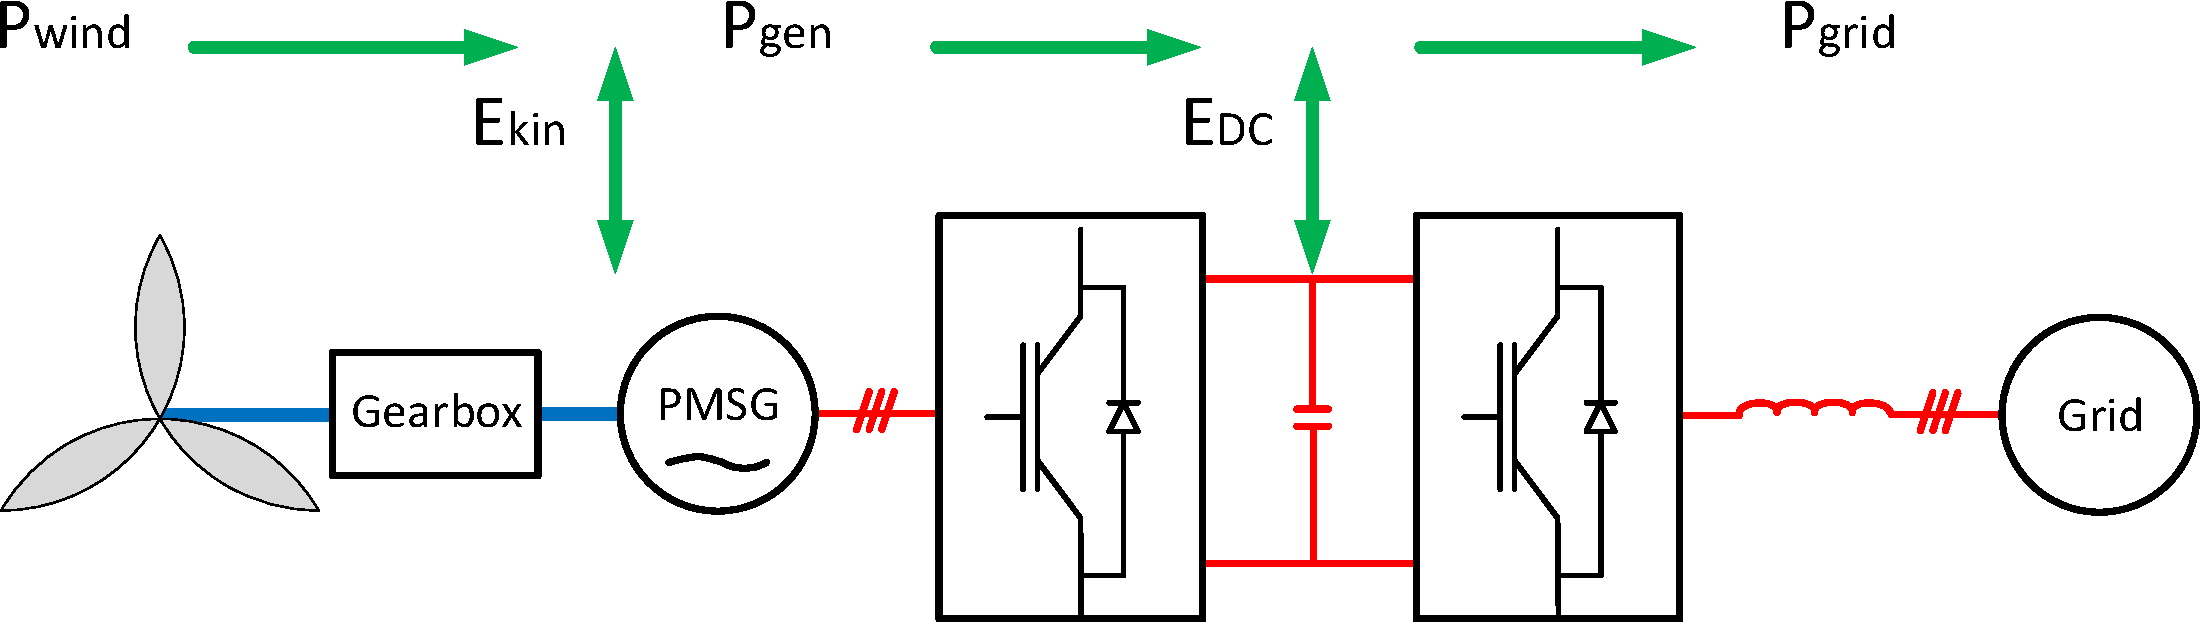
\includegraphics[width=.95\linewidth]{power_flow.pdf}
	\caption{Active Power Flow Diagram}
	\label{power_flow}
\end{figure}
Wind turbine active power can be increased by increasing the generator power $P_{gen}$. This can be achieved by adjusting the generator torque since the active power is proportional to electromagnetic torque. However, the active power is also dependent on the generator rotational speed as in Eq. (\ref{genpower}). The active power can be increased by increasing the torbine torque but the increase is limited by the generator speed. Therefore, the active power increase is also dependent on the wind speed which determines MPPT speed in the steady state.
\begin{equation}
P_{gen}=T_{e} \omega_{m}
\label{genpower}
\end{equation}
Note that the source of the additional power is the kinetic energy stored in the turbine equivalent inertia. Therefore, as soon as the power is increased, the turbine and generator speeds start decreasing. Therefore, the electromagnetic torque should be increased to keep the generator power constant. The time duration that generator power is increased and the initial generator speed will determine the final generator speed as in the Eq. (\ref{finalspeed}).
\begin{equation}
 \int_{t_{i}}^{t_{f}}P_{wind}- \int_{t_{i}}^{t_{f}}P_{gen}=\Delta E_{kin}=\frac{1}{2}J_{tur}(\omega_{f}^2-\omega_{i}^2)
\label{finalspeed}
\end{equation}
As seen from the Eq. (\ref{genpower}), the generator power is the multiplication of generator torque and speed. In the high speeds, the generator speed $\omega_{m}$, cannot be controlled with only the generator torque but also with the pitch angle. In this way, the rated power is not exceeded as in the Eq. (\ref{maxpower}) by maintaining the maximum generator speed and maximum generator torque. However, general practive is employing higher power rating converter than generator active power rating in the variable speed wind turbines. Therefore, higher limit torque can be used in such wind turbine applications by considering the apparent power of the back-to-back converters. Therefore, the maximum power for a wind speed can be defined as in Eq. (\ref{maxxpower}).
\begin{equation}
P_{rated}=T_{P-lim} \omega_{max}
\label{maxpower}
\end{equation}
\begin{equation}
P_{max}=T_{S-lim} \omega_{max}
\label{maxxpower}
\end{equation}
\section{Inertial Support Under Different Wind Speeds}
Active power of the wind turbines is determined by parameters such as wind speed, pitch angle and turbine speed. Therefore, combination of these parameters have importance for a possible inertial support. In other words, wind turbine under high wind scenario has different potential than that under low wind scenario. Likewise, the resultant states of wind turbines for inertial support would be much different. In this chapter, the effect of wind speed will be investigated for inertial support. Active power of wind turbines will be increased by different percentages. The change in generator speed, turbine and generator torques, DC-link voltage and pitch angle, if any, will be observed. Wind turbine used in this study is GE 2.75-103 model, variable speed PMSG.
\subsection{Low Wind Scenario}
\label{sec:lowwind}
The minimum speed of the wind turbine in this scenario is 550 rpm in the high speed side. Wind speed that will capture the maximum power from wind in this generator speed is found out to be 3.12m/s. In this scenario, the kinetic energy stored in the turbine inertia is minimum and calculated in Chapter \ref{chp:4} in Eq. (\ref{kineticenergymin}). This scenario investigates the case where the least amount of kinetic energy exists in the turbine equivalent inertia.\par
\subsubsection{Active Power Limit in Low Wind Scenario}
The electricity grid in the upcoming future might require sudden active power release from wind farms for short time durations. Therefore, it is important to observe the maximum achievable power for inertial support studies. The equation Eq. (\ref{maxxpower}) implies that wind turbine in the low wind speed scenario cannot reach rated active power since the generator speed is much lower than the maximum generator speed. However, the electromagnetic torque in steady state is much lower than the limit torque, $T_{S-lim}$. Therefore, the wind turbine in low speed scenario has the potential for increasing its active power to a significant value. Fig. \ref{low_limit_power} shows the increase of active power to maximum value. The increase is obtained by ensuring the limit torque, $T_{S-lim}$. However, since the generator speed is decreasing, the active power is also decreasing. 

\begin{figure}[h!]
	\centering
	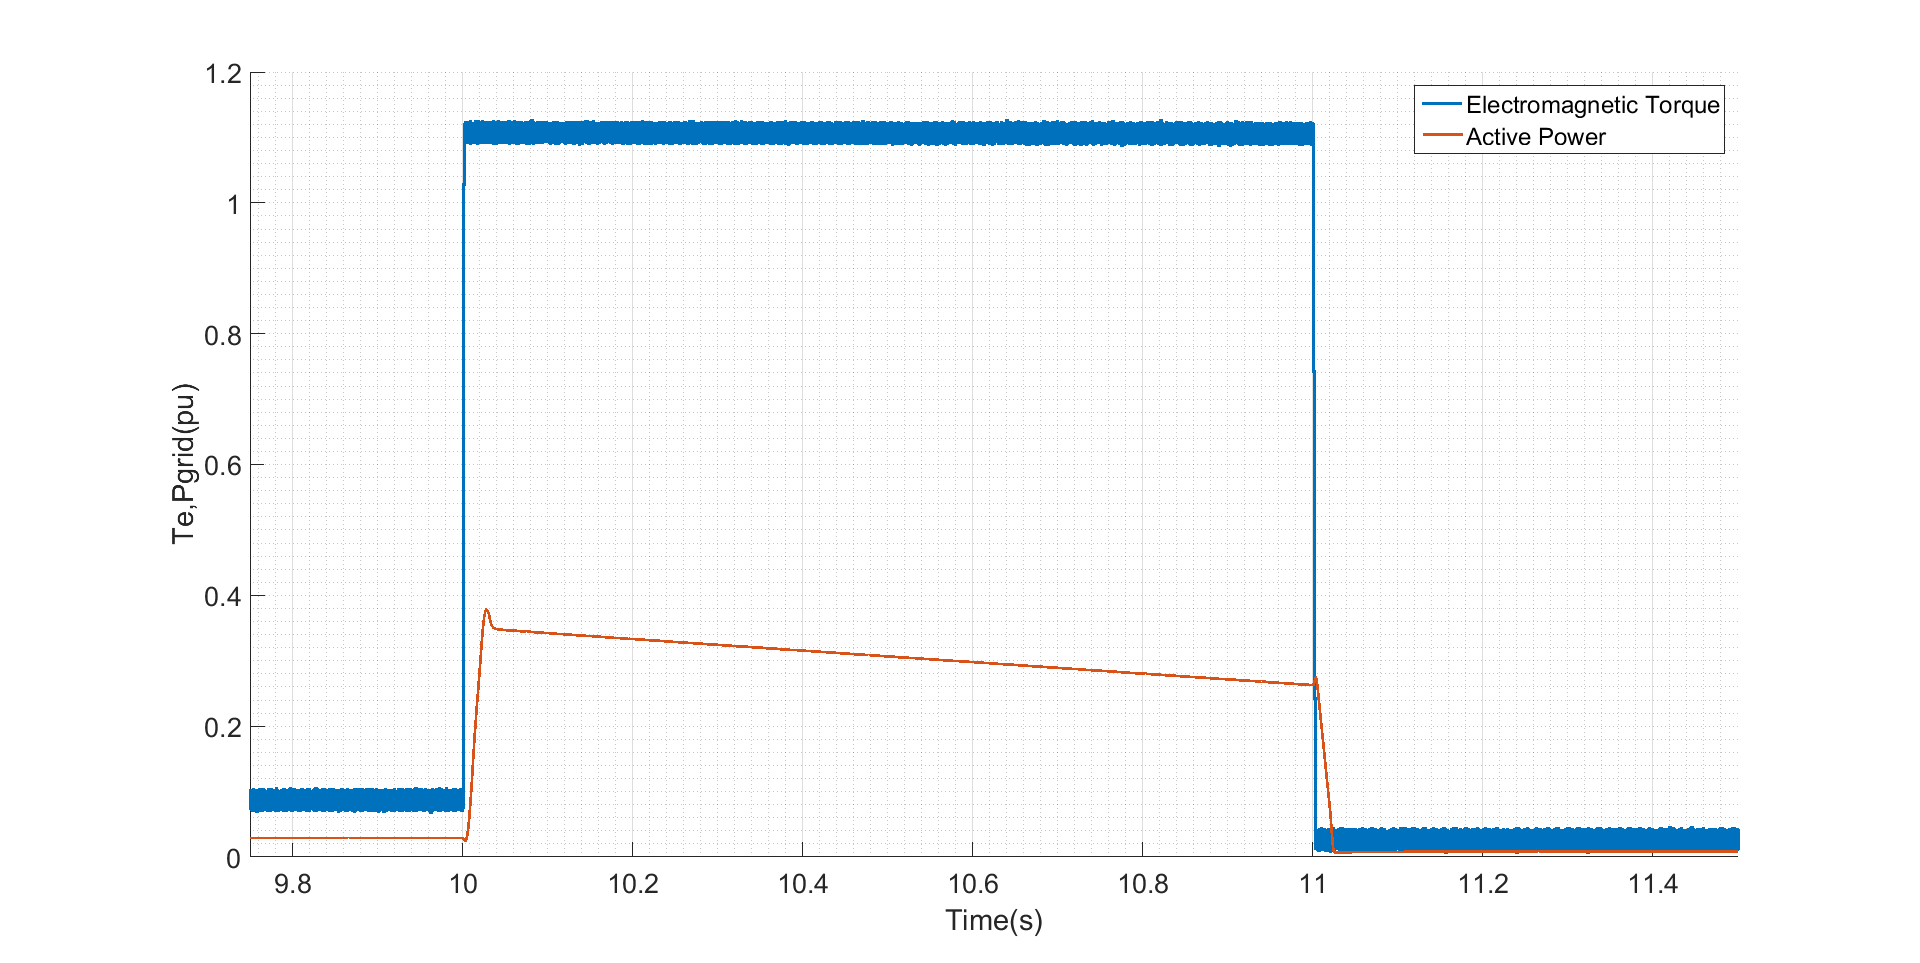
\includegraphics[width=1\linewidth]{power_torque_low_limit.png}
	\caption{Active Power Output of the Wind Turbine for Low Wind Scenario}
	\label{low_limit_power}
\end{figure}
\subsubsection{Active Power in Low Wind Scenario}
The active power of the wind turbine is increased 10\% for three different time intervals as 5, 10 and 20 seconds. The active power output of the wind turbine is given in Fig. \ref{lowactivepowers}. It is observed that turbine power decreases below the nominal value after the support period in order to recover the generator speed. Another observation is the fact that higher support time creates higher dip in the active power in the speed recovery period.\par
\begin{figure}[h!]
	\centering
	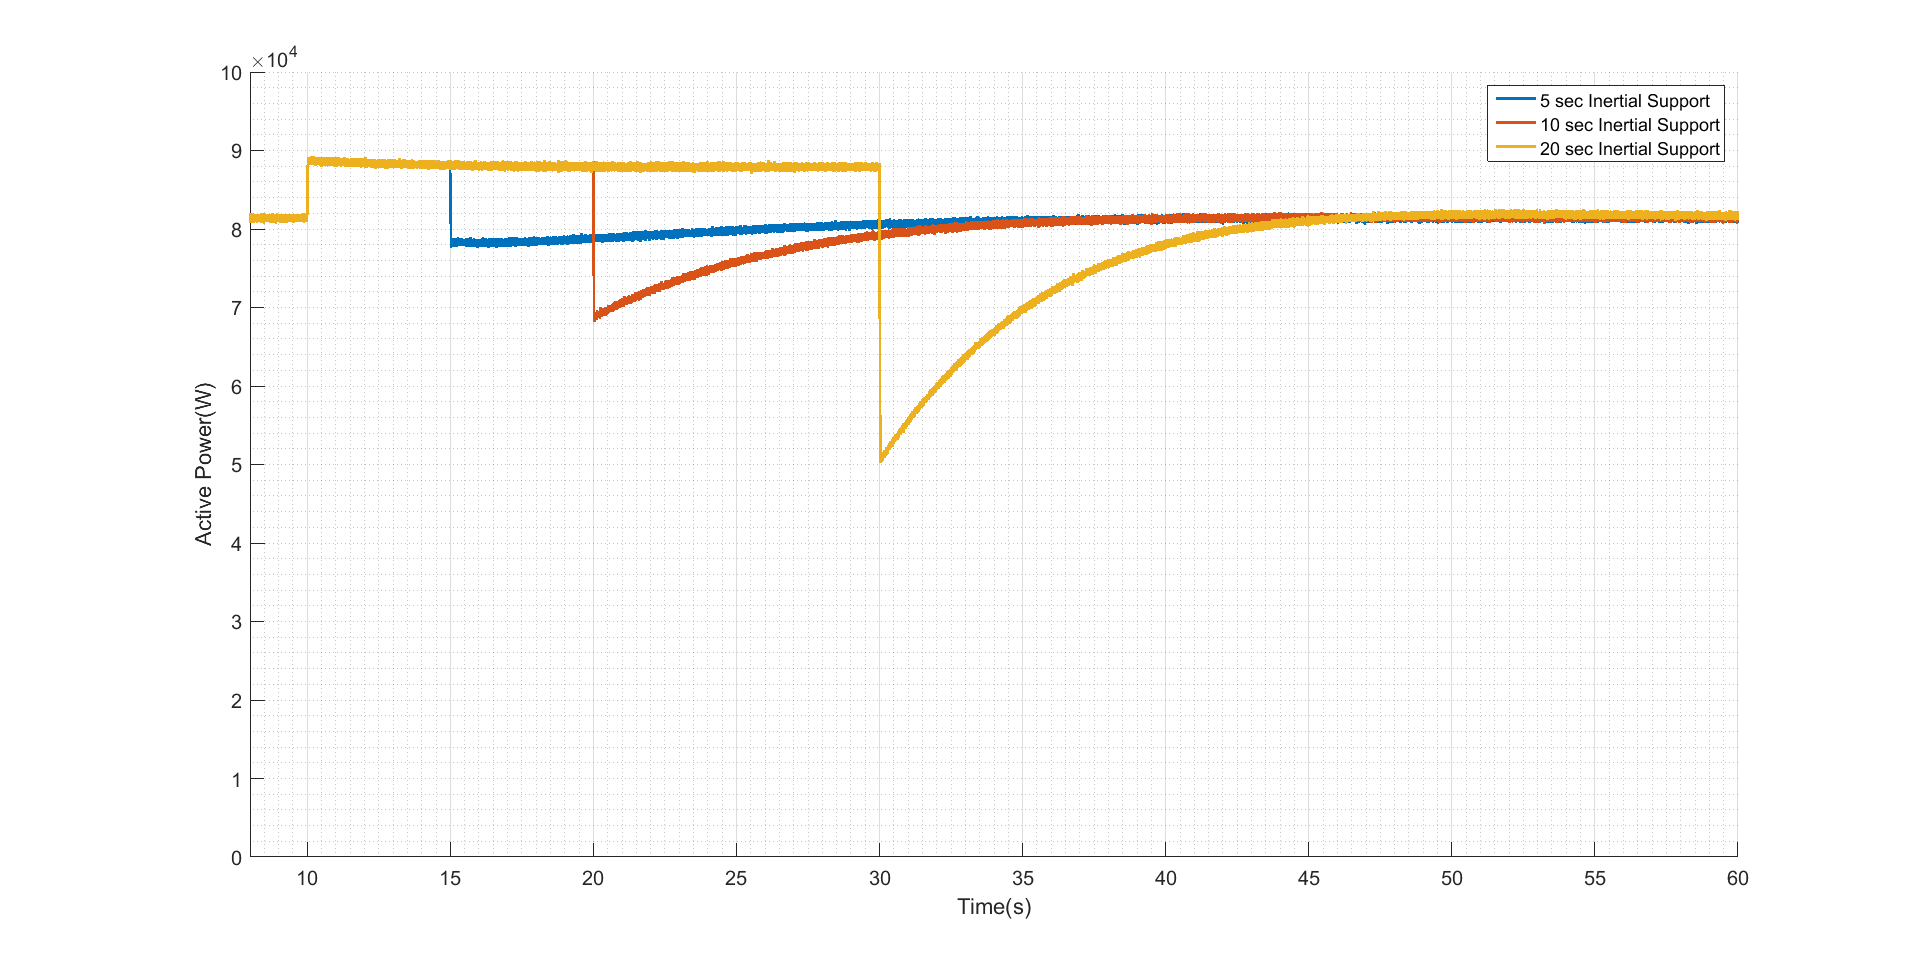
\includegraphics[width=.9\linewidth]{lowwindpowers.png}
	\caption{Active Power Output of the Wind Turbine for Low Wind Scenario}
	\label{lowactivepowers}
\end{figure}
The source of the increased active power in this study is the kinetic energy in the turbine inertia. Therefore, additional active power is extracted from this energy causing a decrease in the wind turbine generator. Generator speed decreases continuously until the support is ended. The generator speeds are shown in Fig. \ref{low_speeds} for three support times.\par
\begin{figure}[h!]
	\centering
	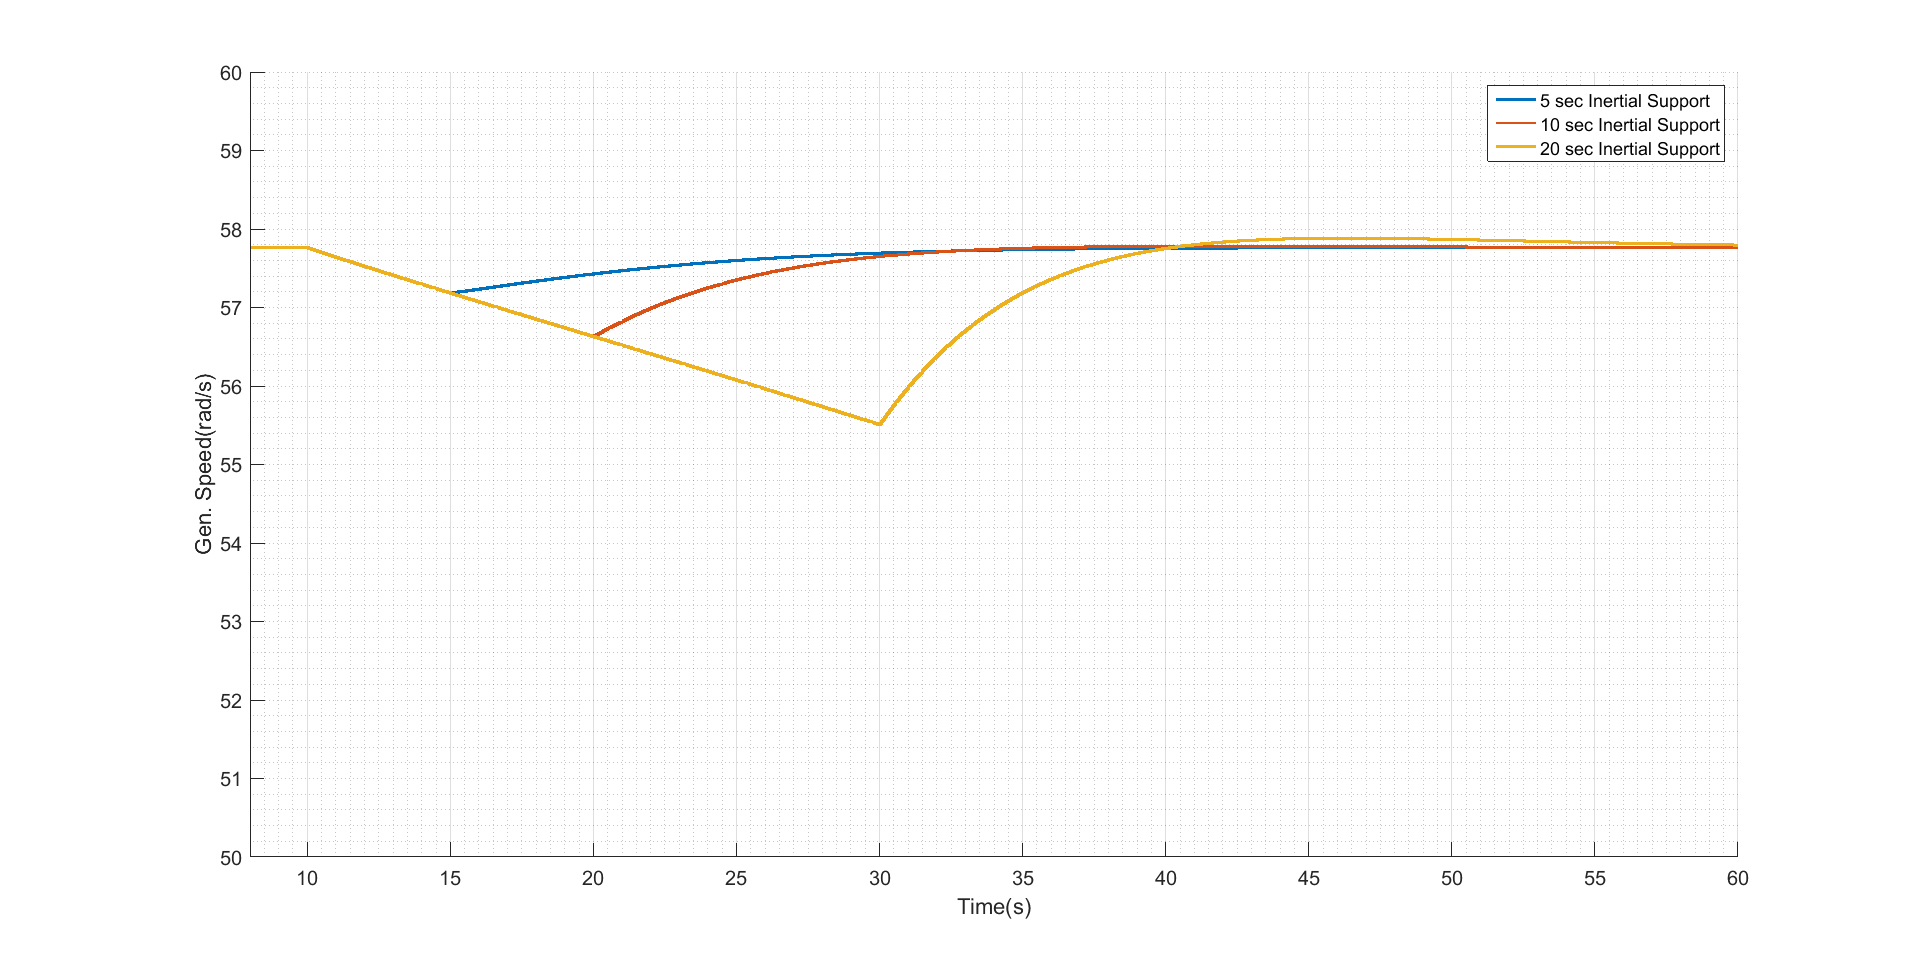
\includegraphics[width=1.0\linewidth]{lowspeeds.png}
	\caption{Generator Speeds of the Wind Turbine for Low Wind Scenario}
	\label{low_speeds}
\end{figure}
The decrease in the generator speed is obtained with an increase in the generator torque. The turbine torque, generator torque and generator speed for 5 seconds support is given in Fig. \ref{low_torques}. The generator torque is increased at t=10s for a time duration of 5 seconds. Turbine torque increases slightly with decreasing speed. However, the increase in the turbine torque is negligible when it is compared to the increase in generator torque as shown in zoomed graph. Therefore, the turbine torque is assumed to be constant for the support period. Turbine and generator torques for the 10 and 20 seconds cases are also shown in Fig. \ref{low_torques2} and Fig. \ref{low_torques3}. 
\begin{figure}[h!]
	\centering
	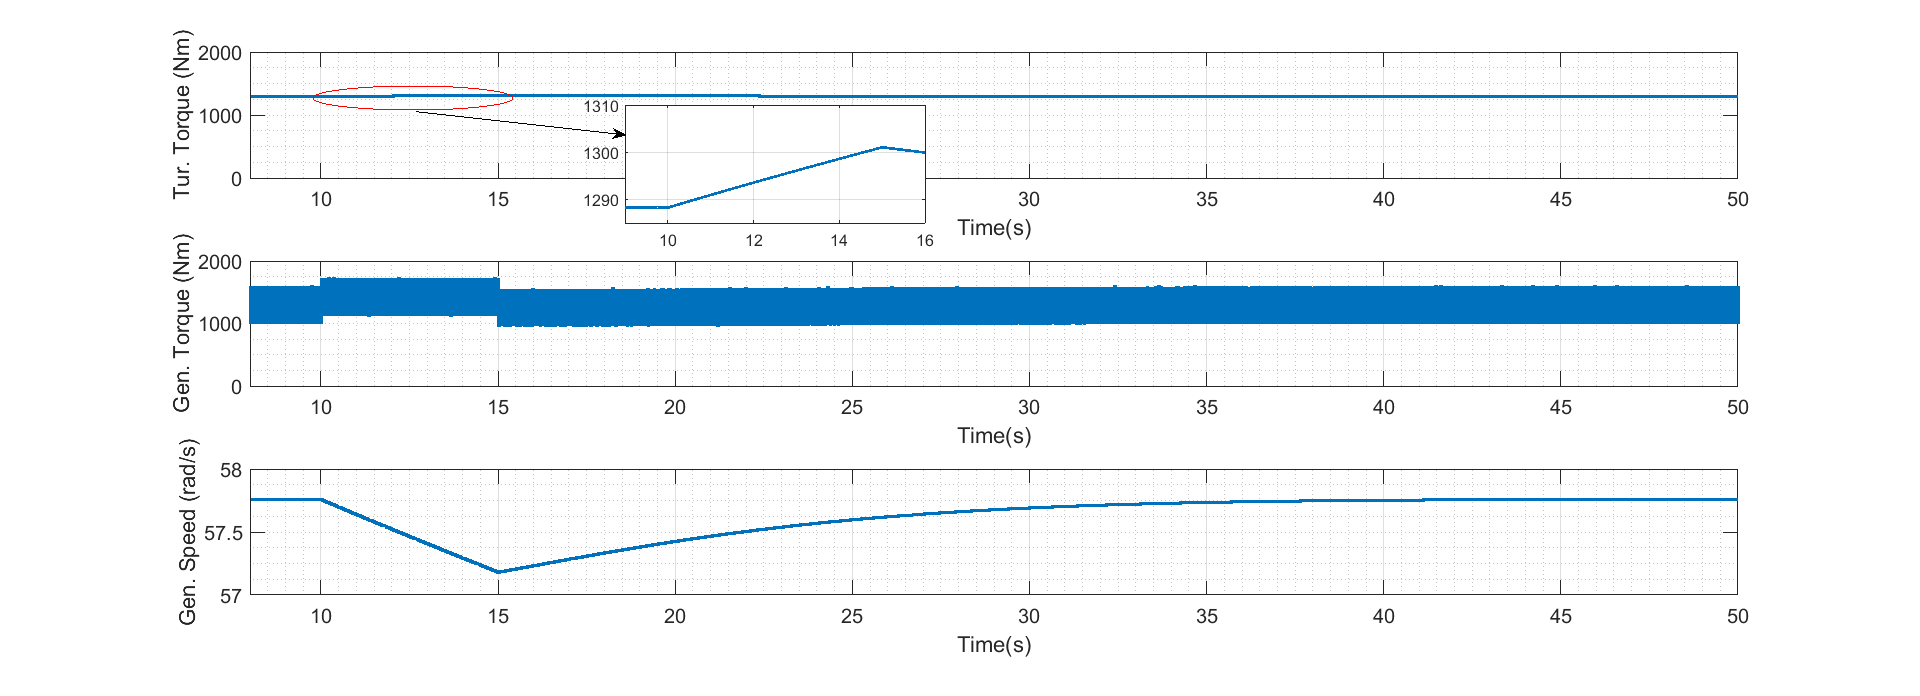
\includegraphics[width=1.0\linewidth]{low_s5_zoomed.png}
	\caption{Turbine Torque, Generator Speed and Torque for 5 Seconds Support under Low Wind Speed}
	\label{low_torques}
\end{figure}
\begin{figure}[h!]
	\centering
	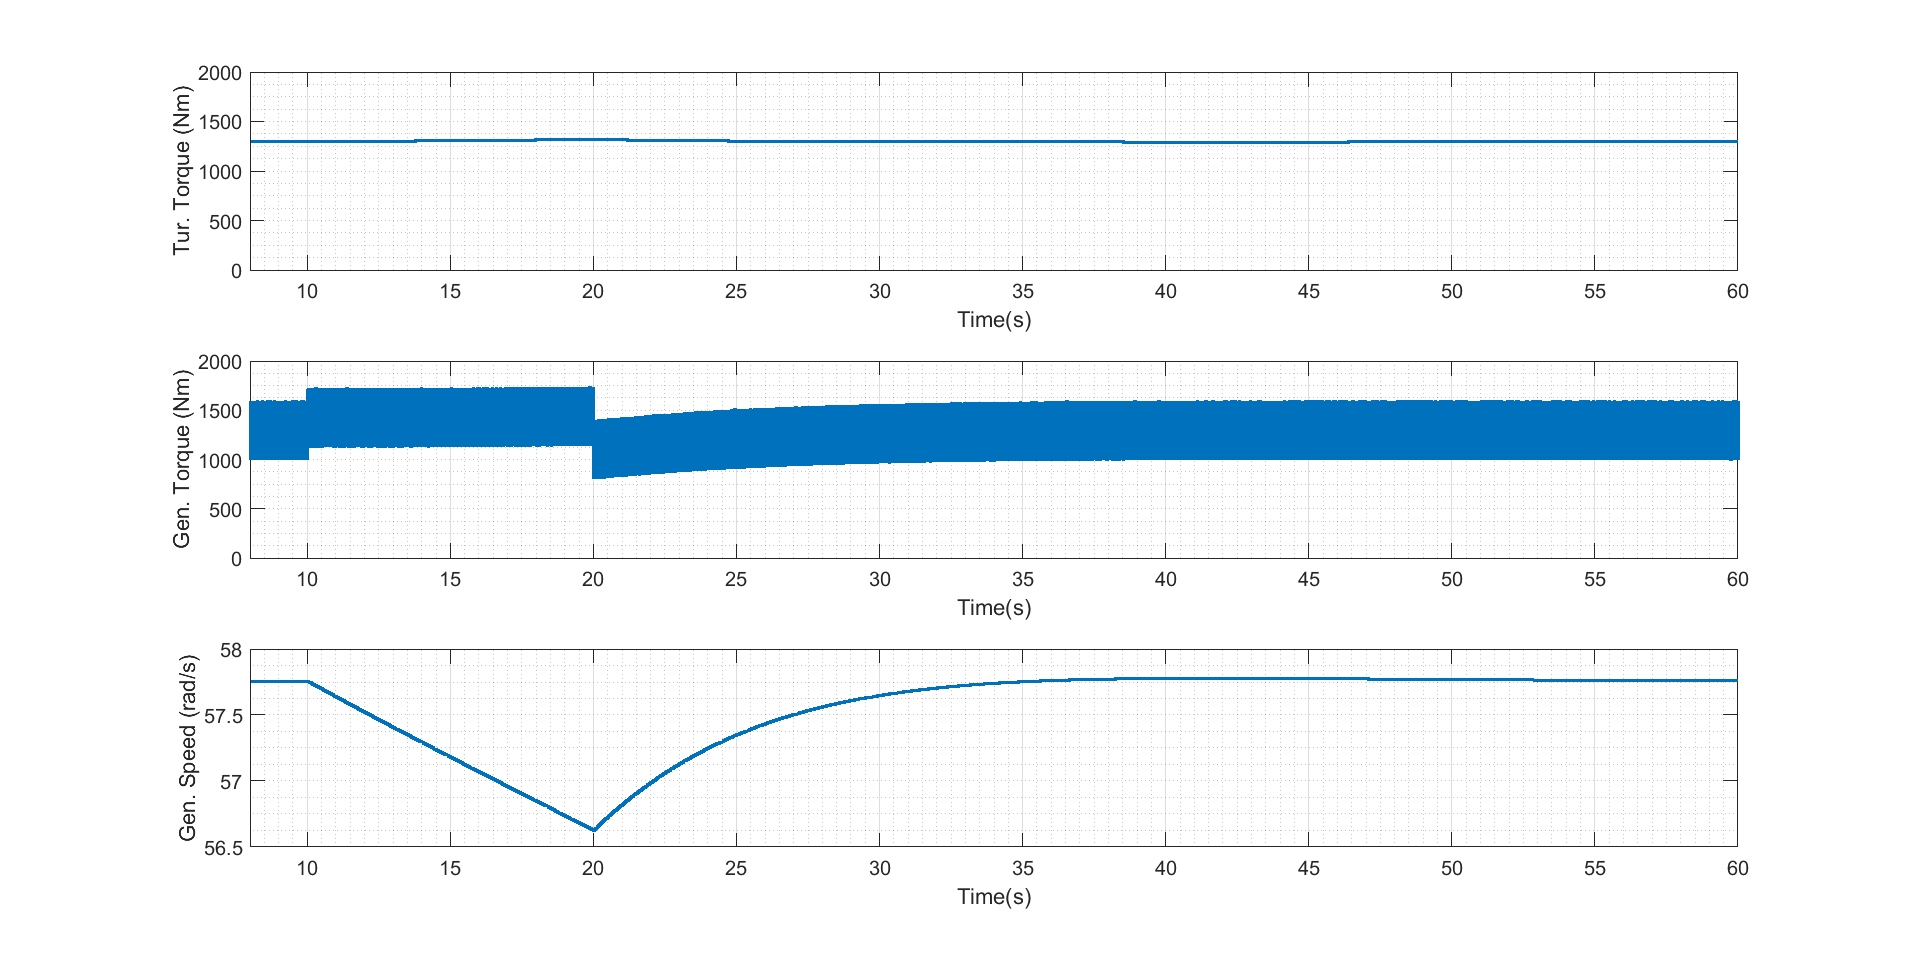
\includegraphics[width=1.0\linewidth]{low_s10.png}
	\caption{Turbine Torque, Generator Speed and Torque for 10 Seconds Support under Low Wind Speed}
	\label{low_torques2}
\end{figure}
\begin{figure}[h!]
	\centering
	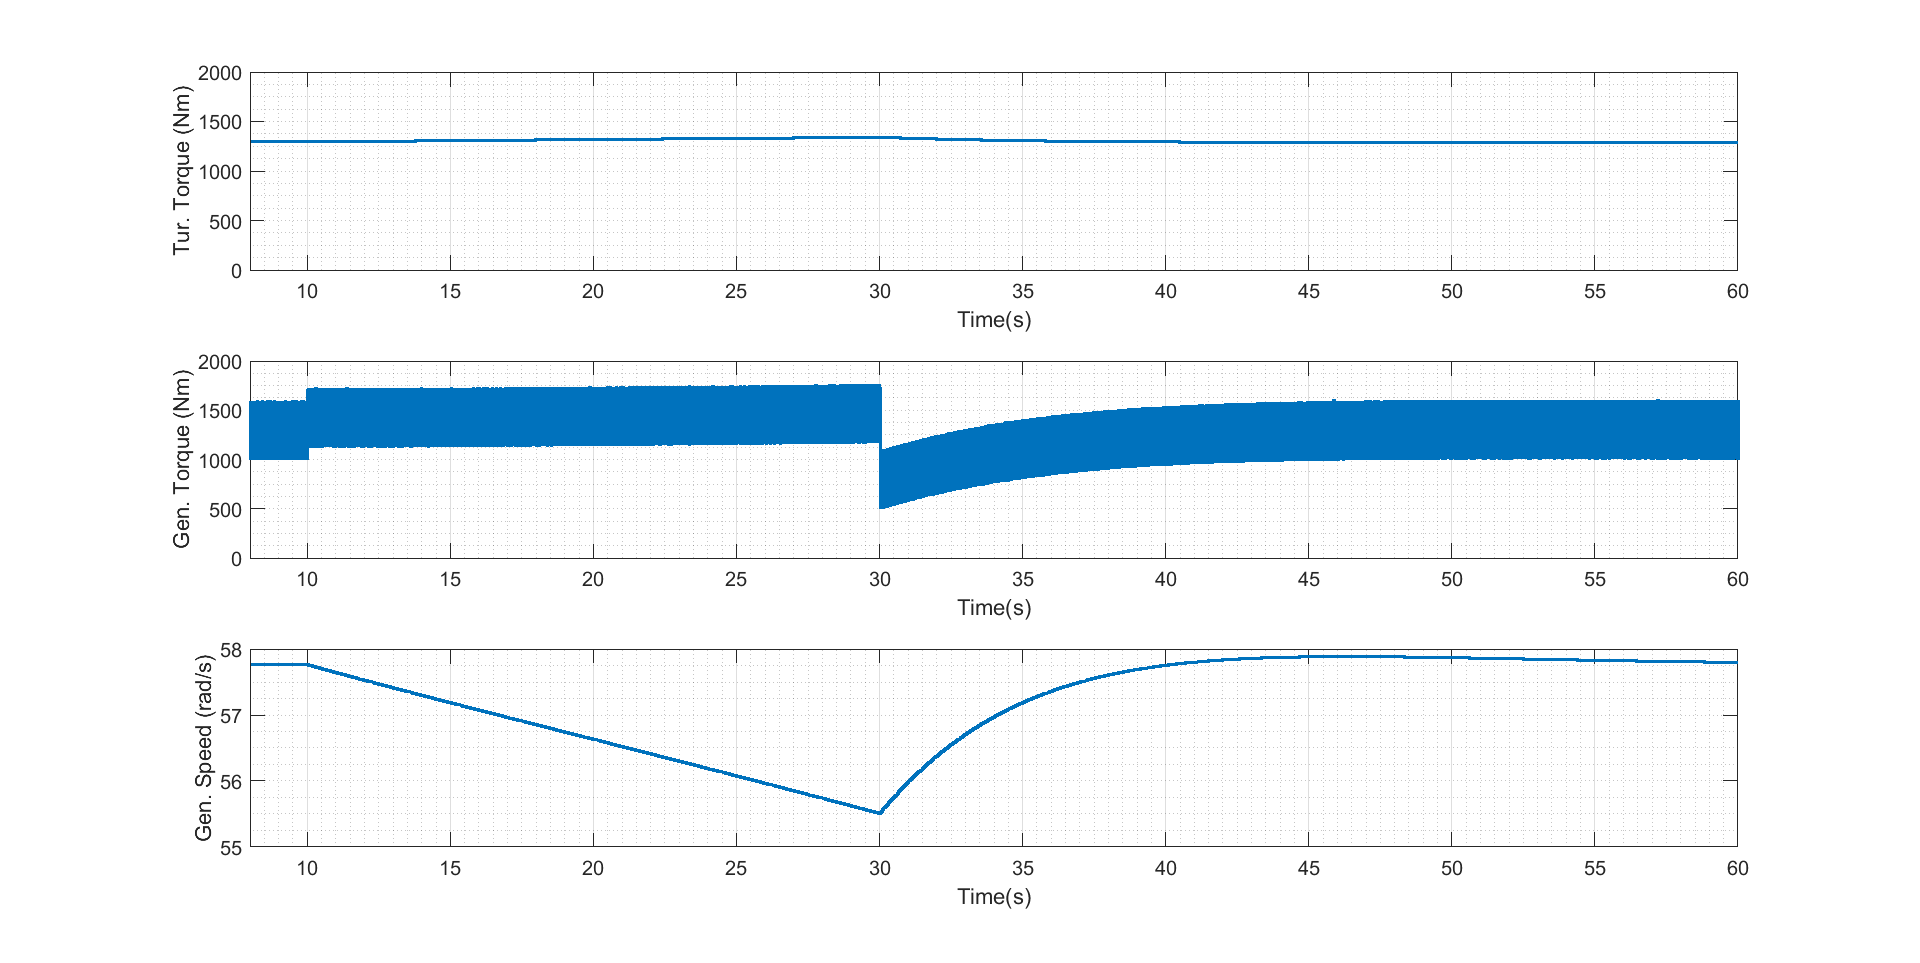
\includegraphics[width=1.0\linewidth]{low_s20.png}
	\caption{Turbine Torque, Generator Speed and Torque for 20 Seconds Support under Low Wind Speed}
	\label{low_torques3}
\end{figure}
Another important criteria on inertial support studies is the DC-Link voltage. When the active power is increased, increased amount of active power is transferred from MSC to GSC. Increased active power should be injected to grid without causing excessive voltage rise on the DC-bus. Note that the voltage rise in the very first seconds in inertial support activation is same for all three support cases. However, the voltage drop will be highest in the 20 seconds case. DC-link voltage for 20 seconds support case is given in Fig. \ref{low_vdc_s20}. The rise on DC-bus voltage can be considered as negligible meanwhile the voltage drops to 0.9995 pu in 20 seconds support case.
\begin{figure}[h!]
	\centering
	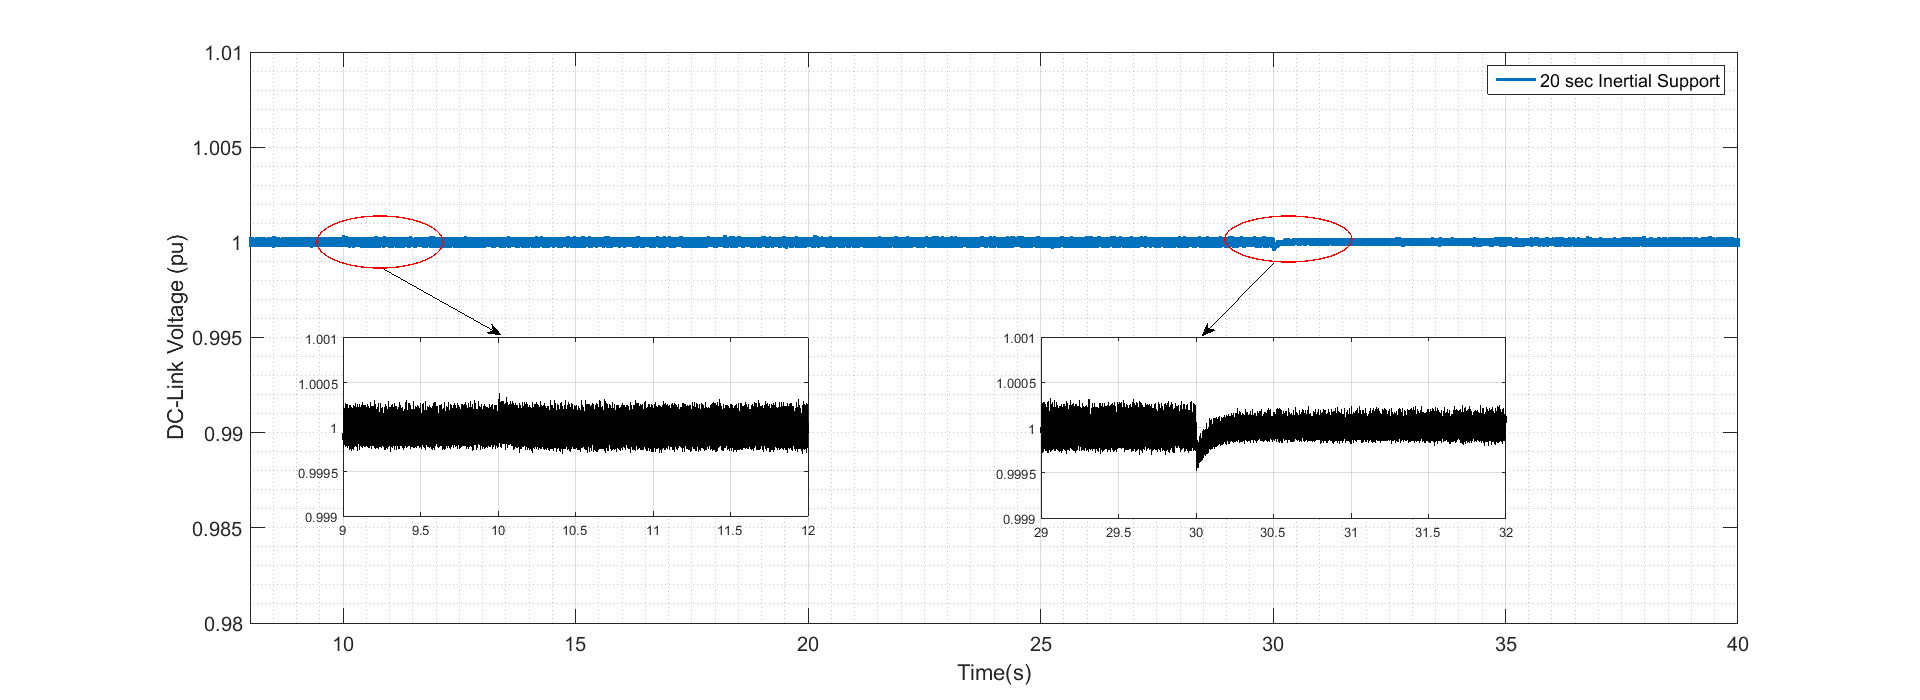
\includegraphics[width=1.0\linewidth]{low_vdc_20.png}
	\caption{DC-Link Voltage for 20 Seconds Support in Low Wind Speed}
	\label{low_vdc_s20}
\end{figure}
\subsection{Medium Wind Scenario}
In the medium wind scenario, wind turbine operated in the middle of the generator speed range. The wind speed is selected as 6m/s in this scenario. 
\subsubsection{Active Power in Medium Wind Scenario}
The active power of the wind turbine is increased by 10\% to provide an inertial support and it is shown in Fig. \ref{midpowers}. The recovery period of shortest support case is much more smoother than the longer ones. When the support time is increased, active power of the wind turbine is almost halved that might cause also problems in frequency stability of the power systems.
\begin{figure}[h!]
	\centering
	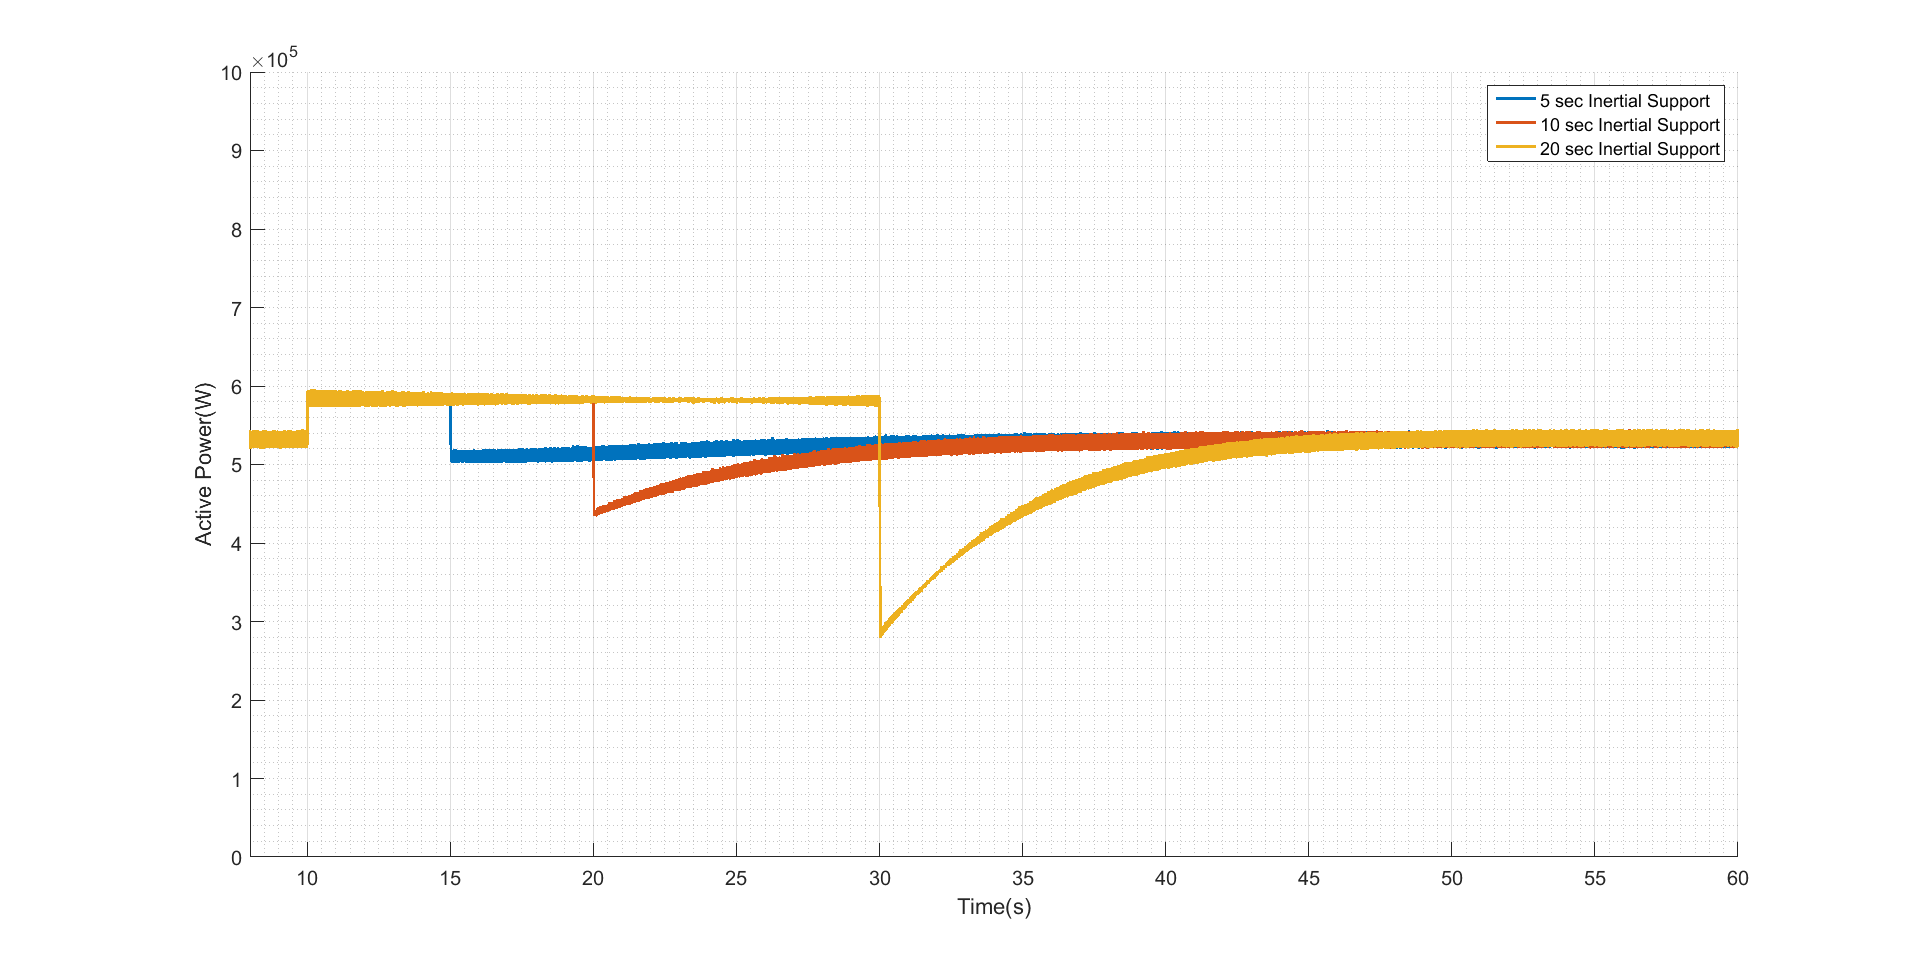
\includegraphics[width=1.0\linewidth]{medium_powers.png}
	\caption{Active Power Output of the Wind Turbine for Medium Wind Scenario}
	\label{midpowers}
\end{figure}
\subsubsection{Generator Speed, Turbine and Generator Torques in Medium Wind Scenario}
In medium wind scenario, higher support time causes decreased active power after the support is ended. The reason is the lower speed value obtained with higher support time. Generator torque is decreased much higher for this case in order to recover the speed. \par
The generator speed, turbine and generator torques are shown in Fig. \ref{mid_torques1}, Fig. \ref{mid_torques2} and Fig.\ref{mid_torques3}. This can be better observed in Fig.\ref{mid_torques3} when the support is ended time at 30 seconds. The negative jump in generator torque crates a negative jump in the active power of the wind turbine since the transferred power is the multiplication of generator torque and generator speed.
\begin{figure}[h!]
	\centering
	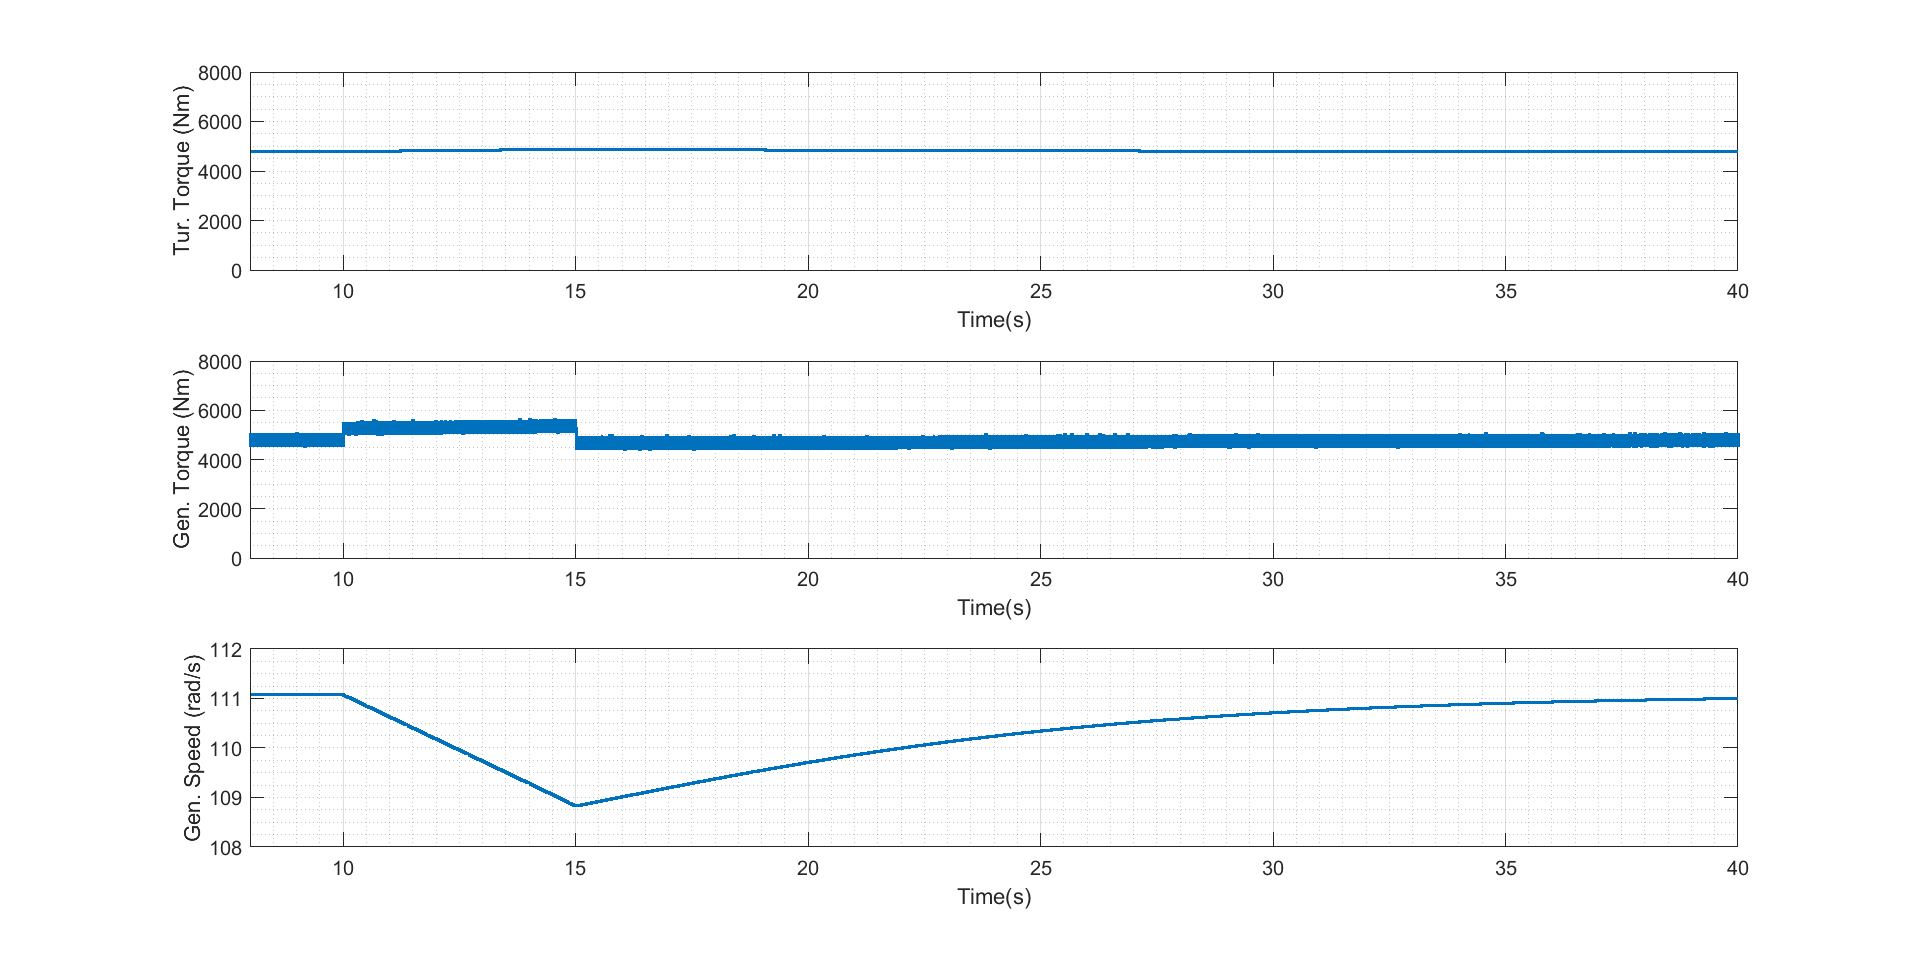
\includegraphics[width=1.0\linewidth]{medium_s5.png}
	\caption{Generator Speed, Generator and Turbine Torques for Medium Wind Scenario for 5 Seconds Support}
	\label{mid_torques1}
\end{figure}
\begin{figure}[h!]
	\centering
	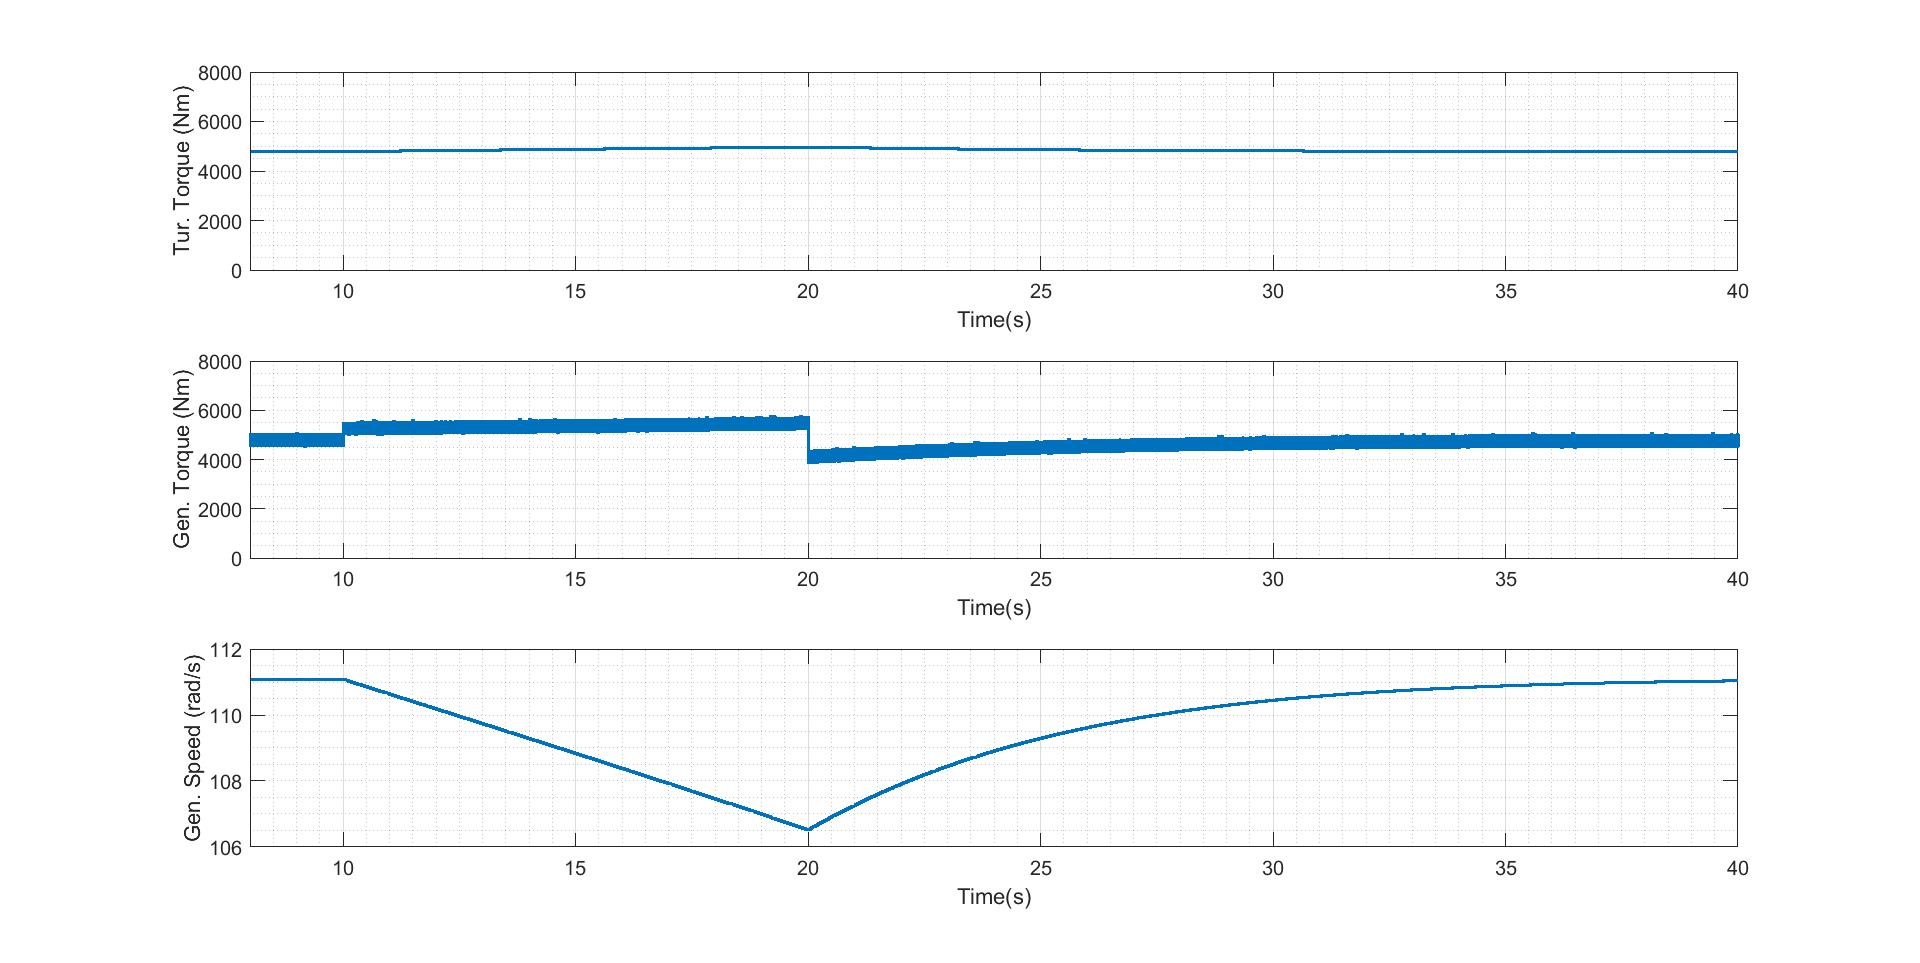
\includegraphics[width=1.0\linewidth]{medium_s10.png}
	\caption{Generator Speed, Generator and Turbine Torques for Medium Wind Scenario for 10 Seconds Support}
	\label{mid_torques2}
\end{figure}
\begin{figure}[h!]
	\centering
	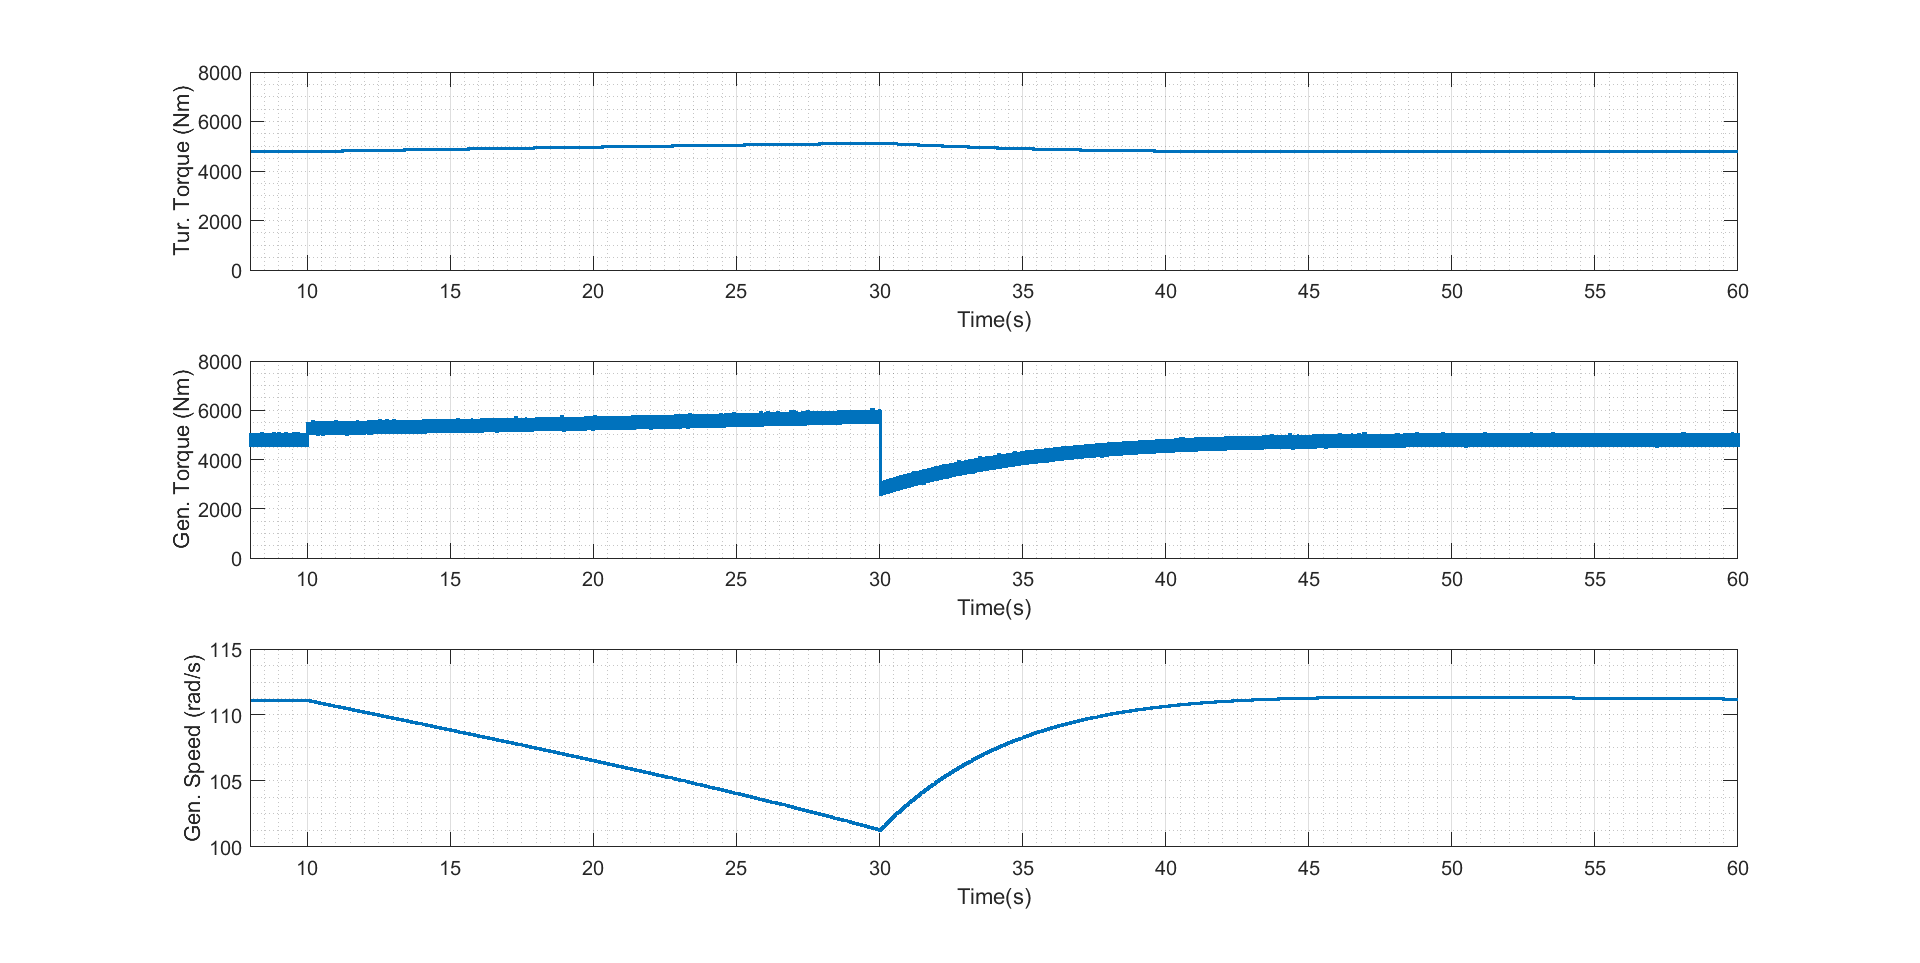
\includegraphics[width=1.0\linewidth]{medium_s20.png}
	\caption{Generator Speed, Generator and Turbine Torques for Medium Wind Scenario for 20 Seconds Support}
	\label{mid_torques3}
\end{figure}
\subsubsection{DC-Link Voltage in Medium Wind Scenario}
The variation of DC-bus voltage with inertial support is shown in Fig. \ref{med_vdc_s20}. The support is activated in time 10 seconds. The rise on the DC-bus voltage is negligible as in the case of low wind scenario. However, the voltage drop at the end of support is much more significant than that of low wind scenario. 
\begin{figure}[h!]
	\centering
	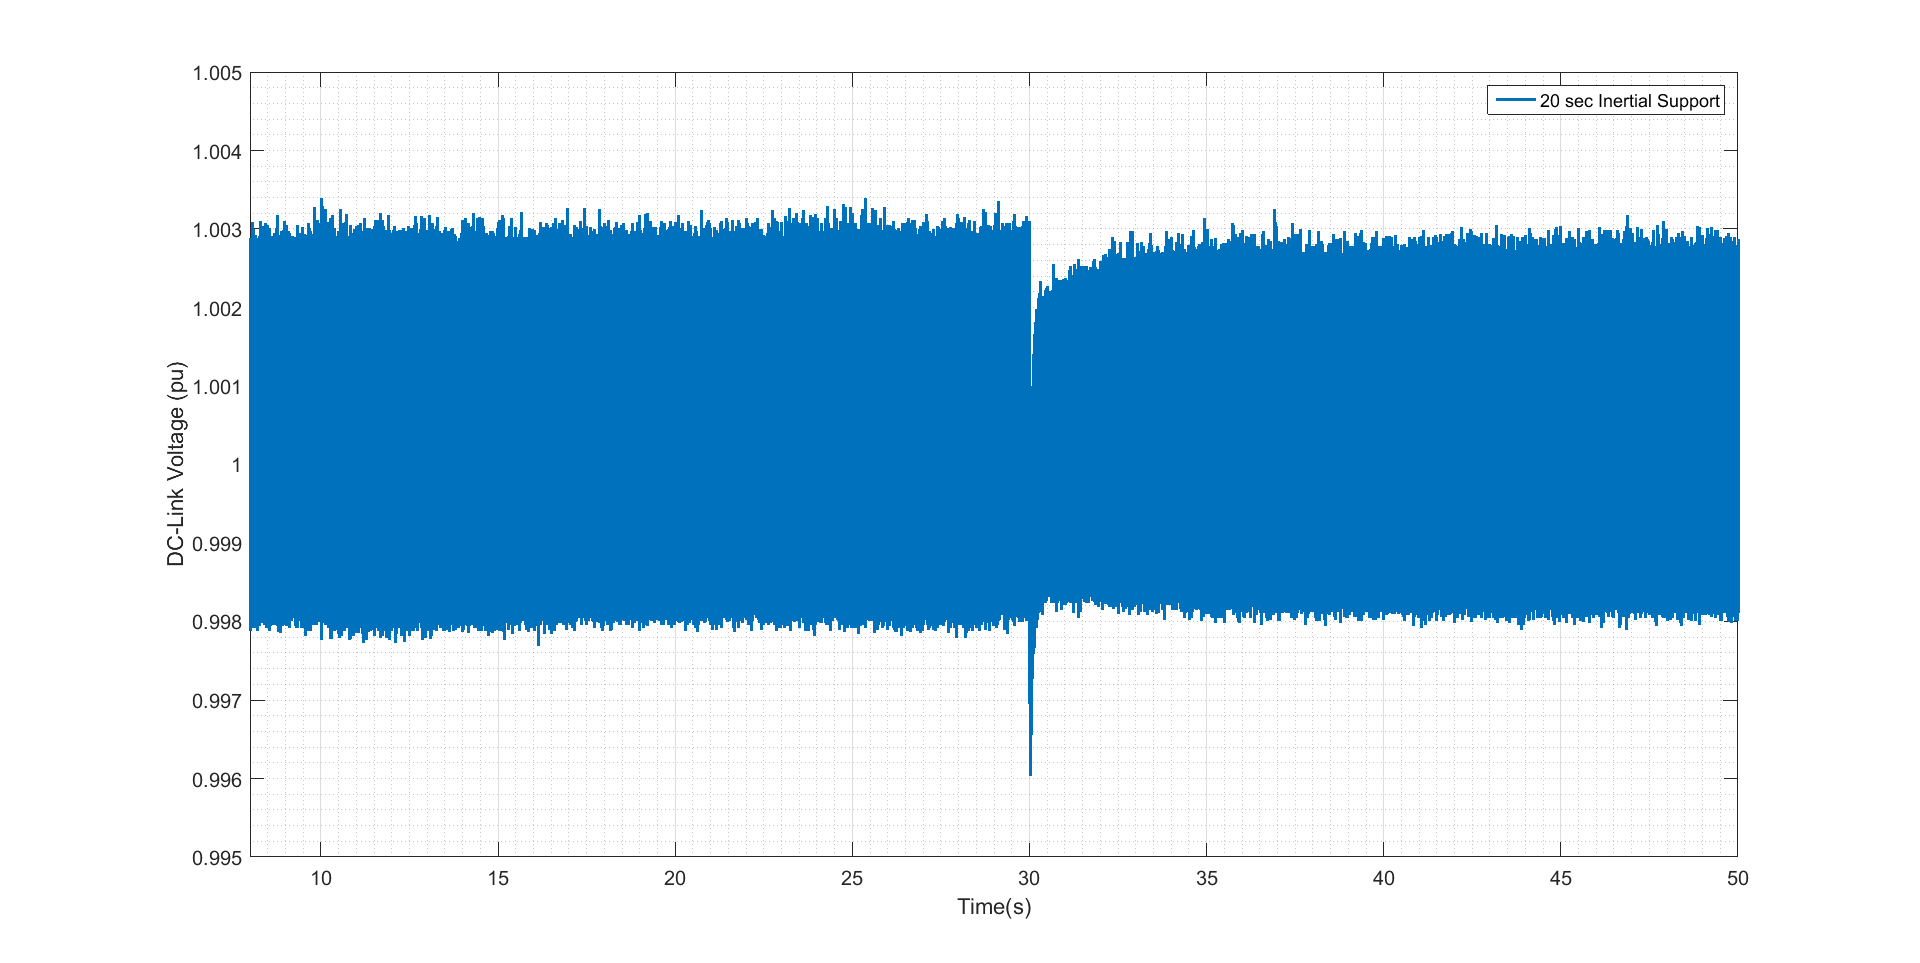
\includegraphics[width=1.0\linewidth]{medium_s20_vdc.png}
	\caption{DC-Link Voltage for 20 Seconds Support in Medium Wind Speed}
	\label{med_vdc_s20}
\end{figure}
\subsection{High Wind Scenario}
In this section, wind turbine operation with high wind speed is investigated. In the high speed operation, the wind turbine injects its maximum power to grid. However, the generator reference speed is the maximum wind speed. Therefore, wind turbine operation is from MPPT operation. Another difference in this section is the pitch angle that curtail wind power and ensure that the generator speed is kept at its maximum. The wind speed in this scenario is selected as 11.4m/s.\par
\subsubsection{Active Power in High Wind Scenario}
Wind turbines are able to provide inertial support in high wind speed as long as converter power rating is higher than the wind turbine power rating. The wind turbine investigated throughout the study has a converter rating of 3.04MVA meanwhile turbine power rating of 2.75MW. Therefore, active power output can be increased up to 3.04MW during support interval. Otherwise, wind turbine cannot provide inertial support for high wind speeds. The active power of the wind turbine is increased by 10\% with three different time intervals. The active powers are shown in Fig. \ref{high_powers}.\par
\begin{figure}[h!]
	\centering
	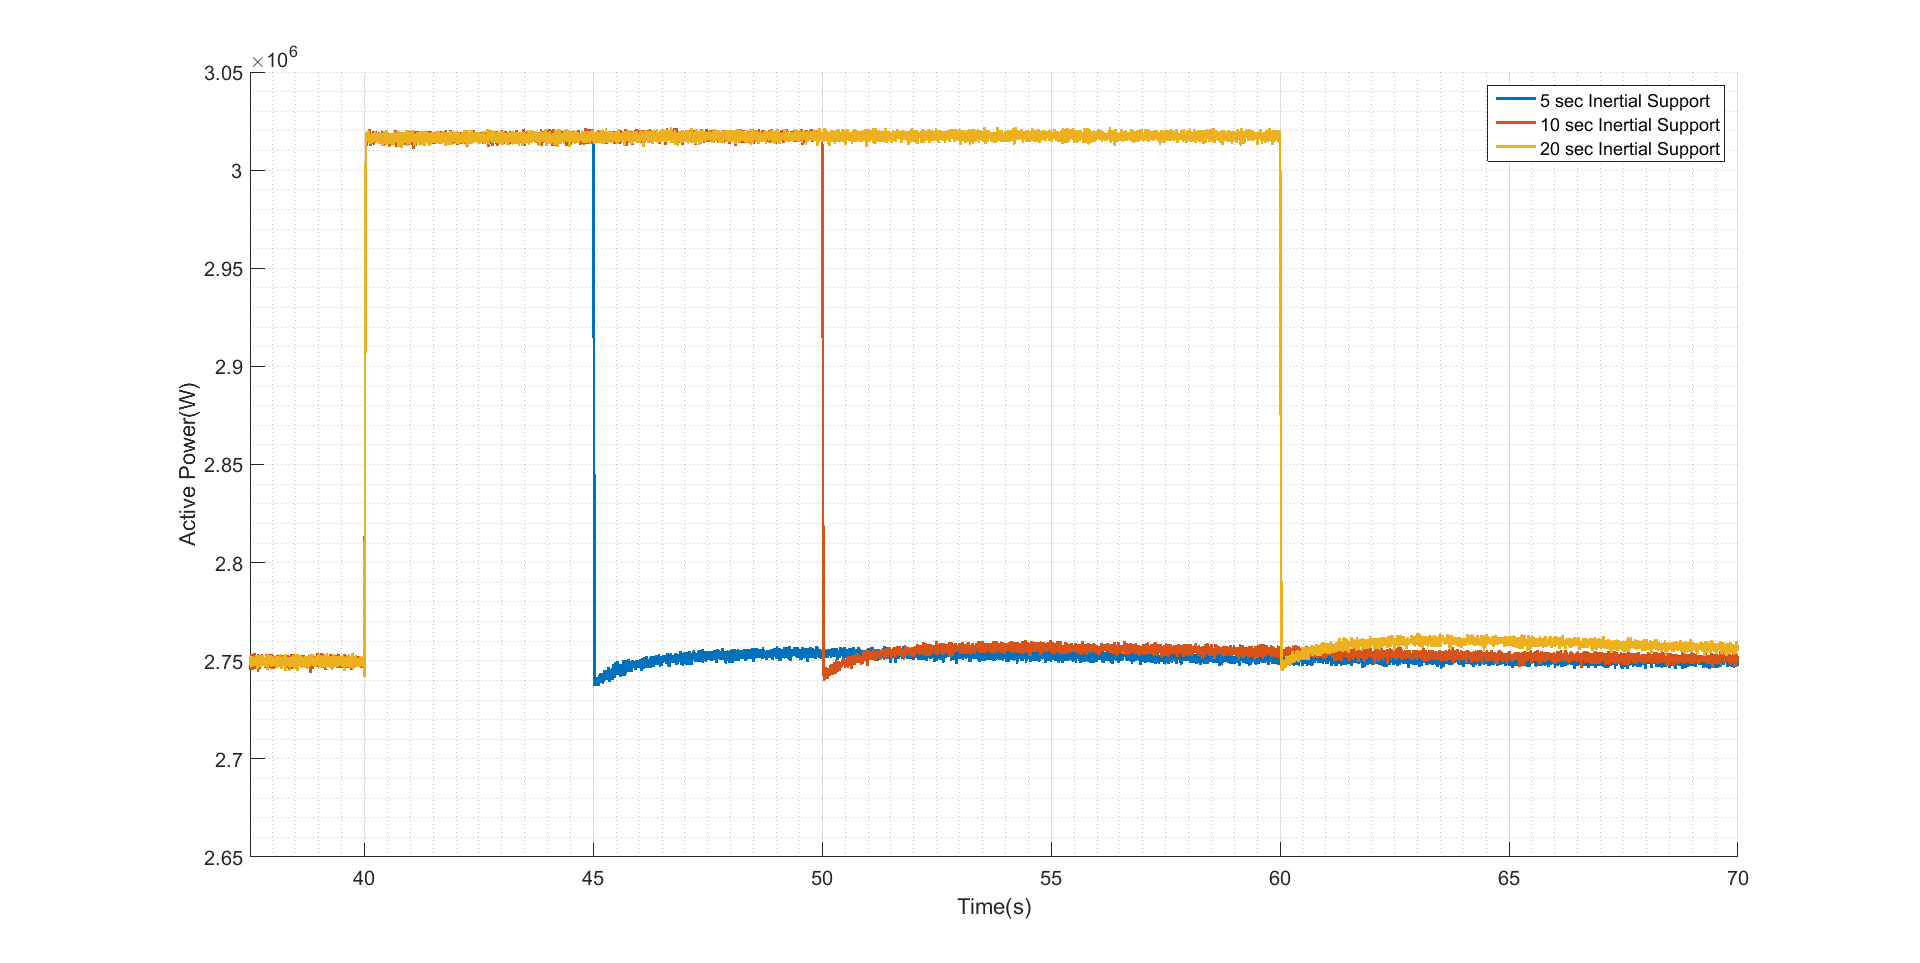
\includegraphics[width=1.0\linewidth]{high_s5_10_20_power.png}
	\caption{Active Power Output of the Wind Turbine for High Wind Scenario}
	\label{high_powers}
\end{figure}
An interesting observation in high wind scenario is that there is no speed recovery process. As soon as the speed is decreased, the pitch controller decreases the blade angle which causes an increase in turbine torque. Therefore, in this case, turbine power decreases back to normal rather than a lower power value as in the other scenarios.
\subsubsection{Generator Speed, Turbine and Generator Torques in High Wind Scenario}
In the high wind case, the generator torque hits the limit defined for normal operating conditions. This is why generator speed is regulated with the help of blade angle. Therefore, pitch angle is also important in this section. Generator speed, turbine and generator torques as well as pitch angle for 5, 10 and 20 seconds support cases are shown in Fig. \ref{high_s5}, Fig. \ref{high_s10} and Fig. \ref{high_s20}. Generator speed starts decreasing when the generator torque is increased. However, the pitch controller decreases the blade angle since the generator speed is below the maximum speed. Therefore, the generator speed rises when the pitch angle is decreased. Note that pitch servo acts slower than the generator torque increase time. This is why the generator speed decreases until the pitch angle is decreased. Generator speed might not be disturbed if the pitch controller is able act fast enough.\par
\begin{figure}[h!]
	\centering
	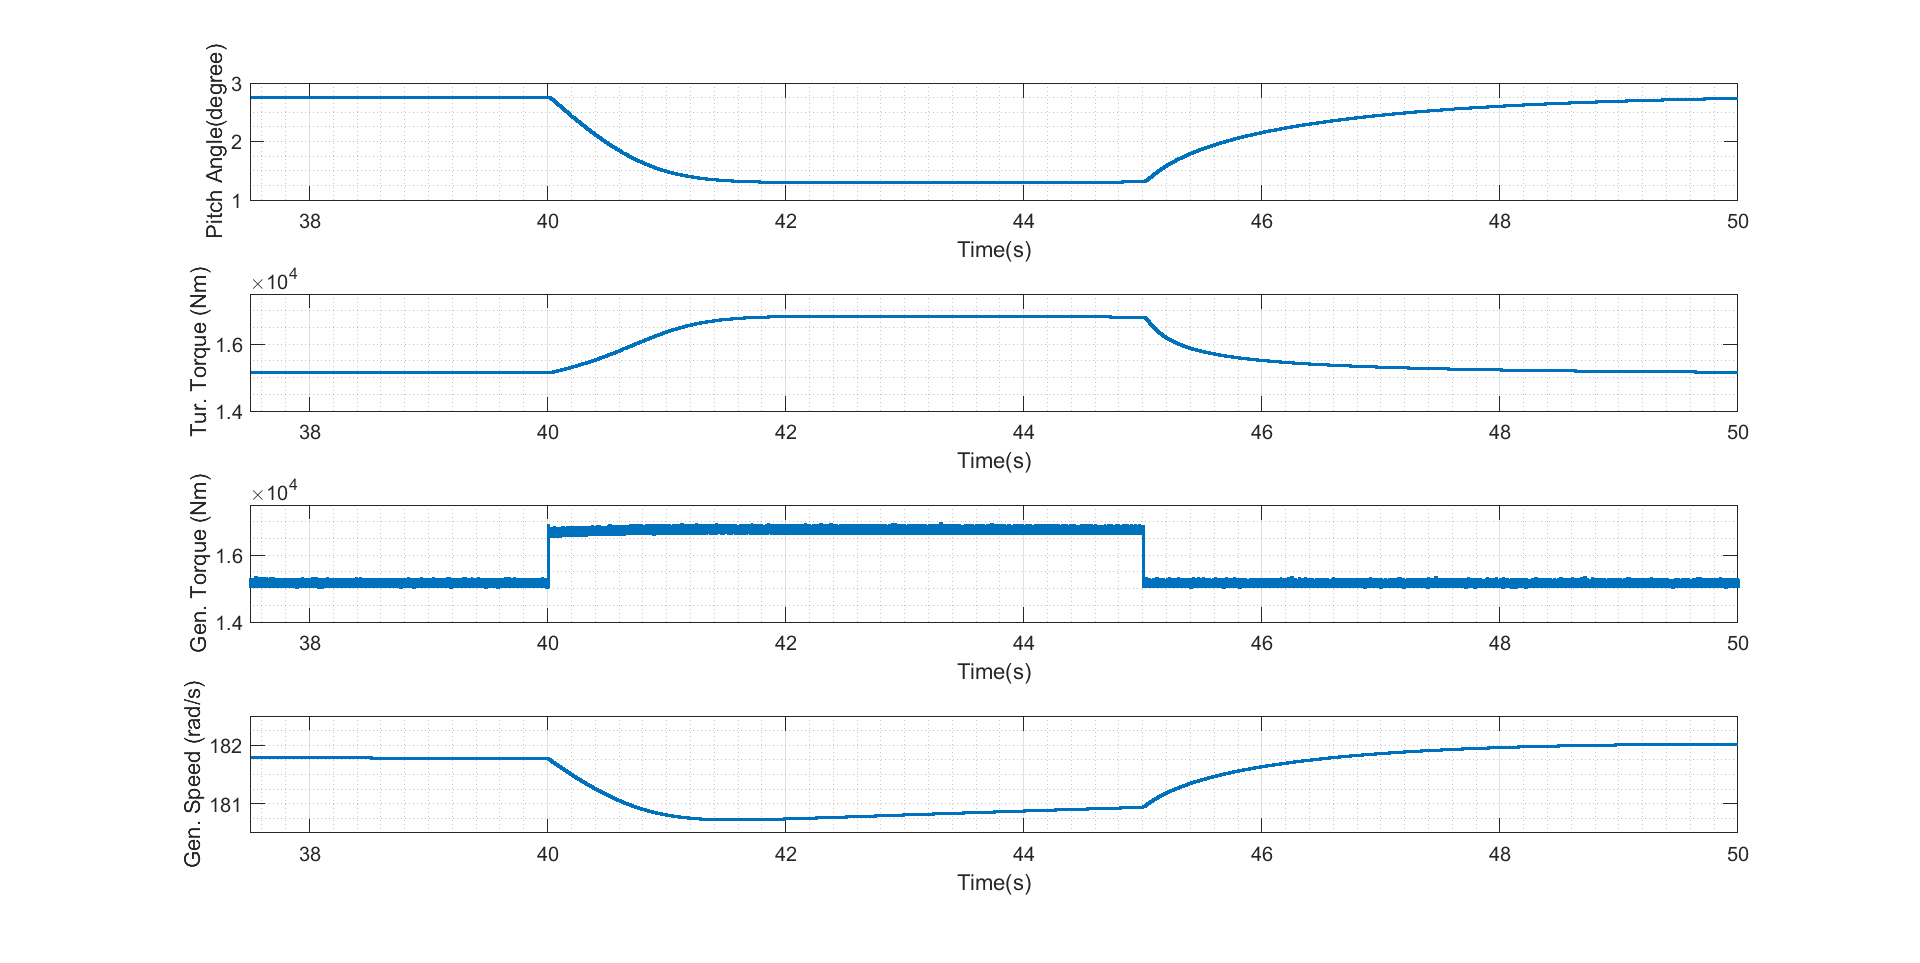
\includegraphics[width=1.0\linewidth]{high_s5_with_torques.png}
	\caption{Pitch Angle, Generator Speed, Generator and Turbine Torques for High Wind Scenario for 5 Seconds Support}
	\label{high_s5}
\end{figure}
\begin{figure}[h!]
	\centering
	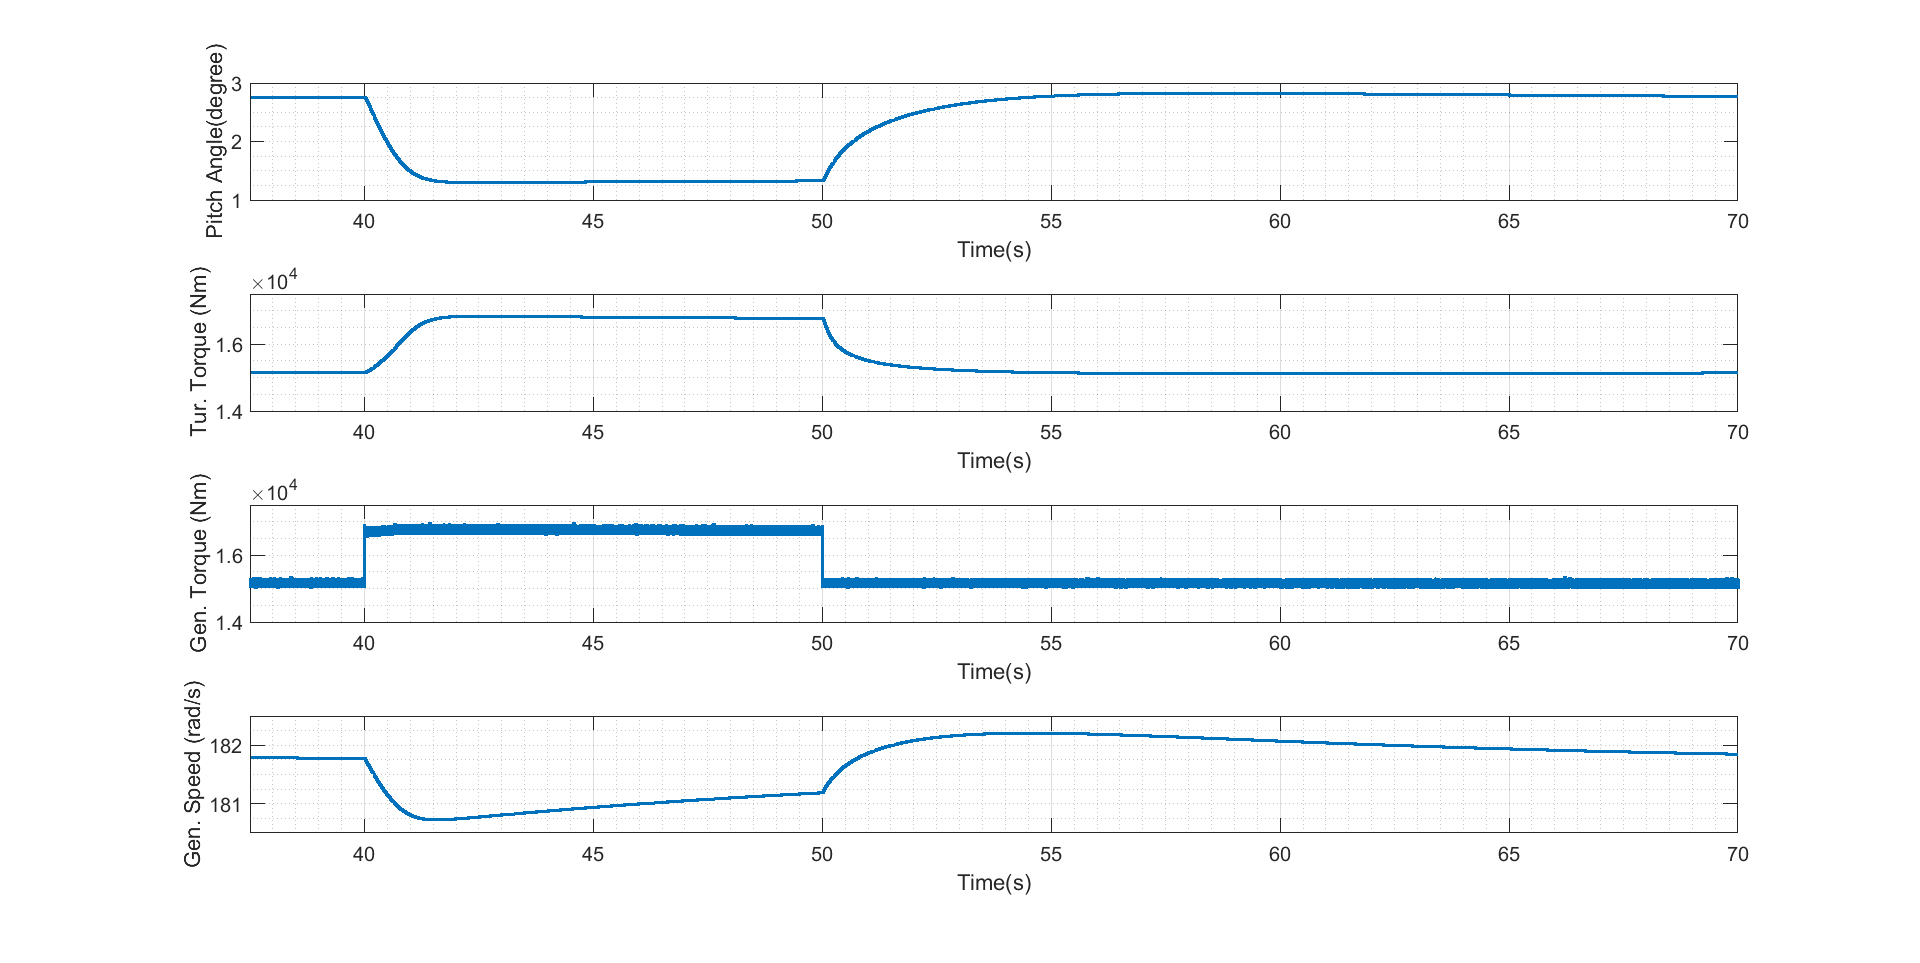
\includegraphics[width=1.0\linewidth]{high_s10_with_torques.png}
	\caption{Pitch Angle, Generator Speed, Generator and Turbine Torques for High Wind Scenario for 10 Seconds Support}
	\label{high_s10}
\end{figure}
\begin{figure}[h!]
	\centering
	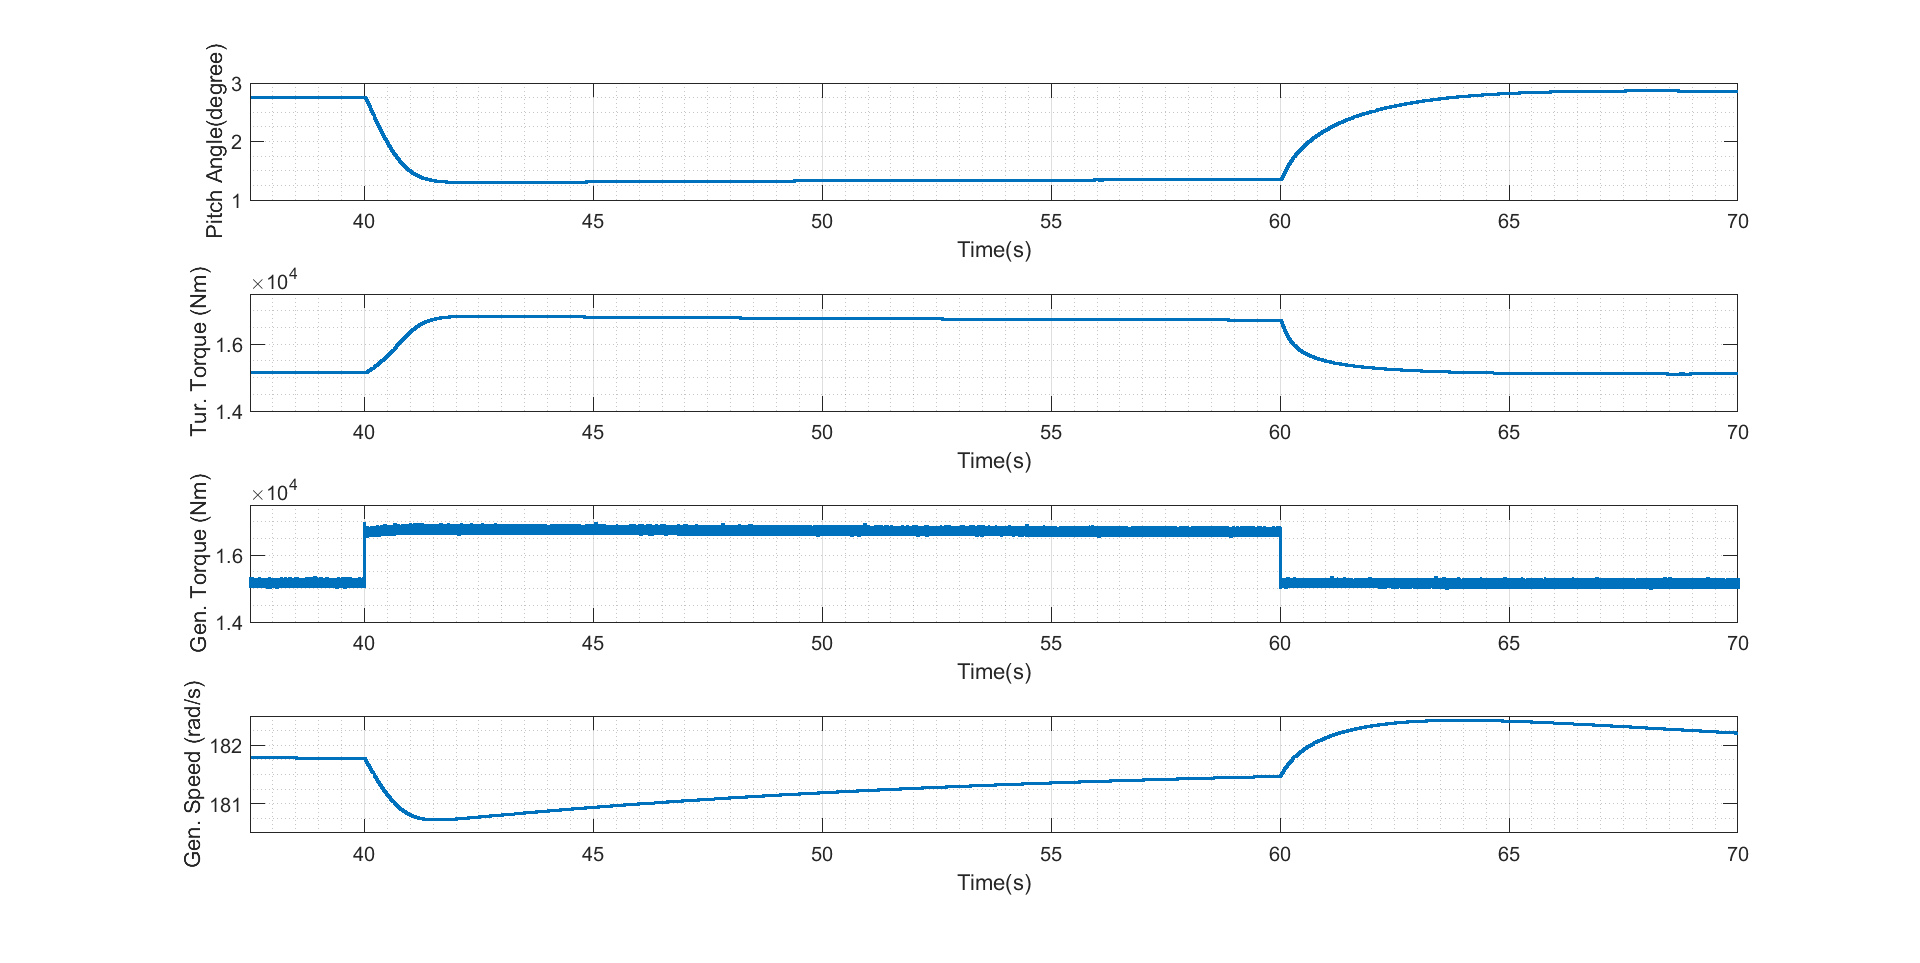
\includegraphics[width=1.0\linewidth]{high_s20_with_torques.png}
	\caption{Pitch Angle, Generator Speed, Generator and Turbine Torques for High Wind Scenario for 20 Seconds Support}
	\label{high_s20}
\end{figure}
In high wind scenario, generator speed rises towards the maximum generator speed thanks to the decrease in blade angle. If the support time is increased, the generator speed will reach the maximum speed, and will stay constant with a new pitch angle. 
\subsubsection{DC-Link Voltage in High Wind Scenario}
The DC-bus voltage is not affected from inertial support on low speed scenario. However, the nominal power and additional power in low speed case is much smaller than that of high wind scenario. The effect of inertial support in high wind case is shown in Fig. \ref{high_s20_vdc}. Nonetheless, the DC-bus voltage is between the range of 0.996 and 1.004 pu in high wind scenario. Note that wind turbines encounter such variations in the DC-bus voltage when the wind speed changes during daily operation. 
\begin{figure}[h!]
	\centering
	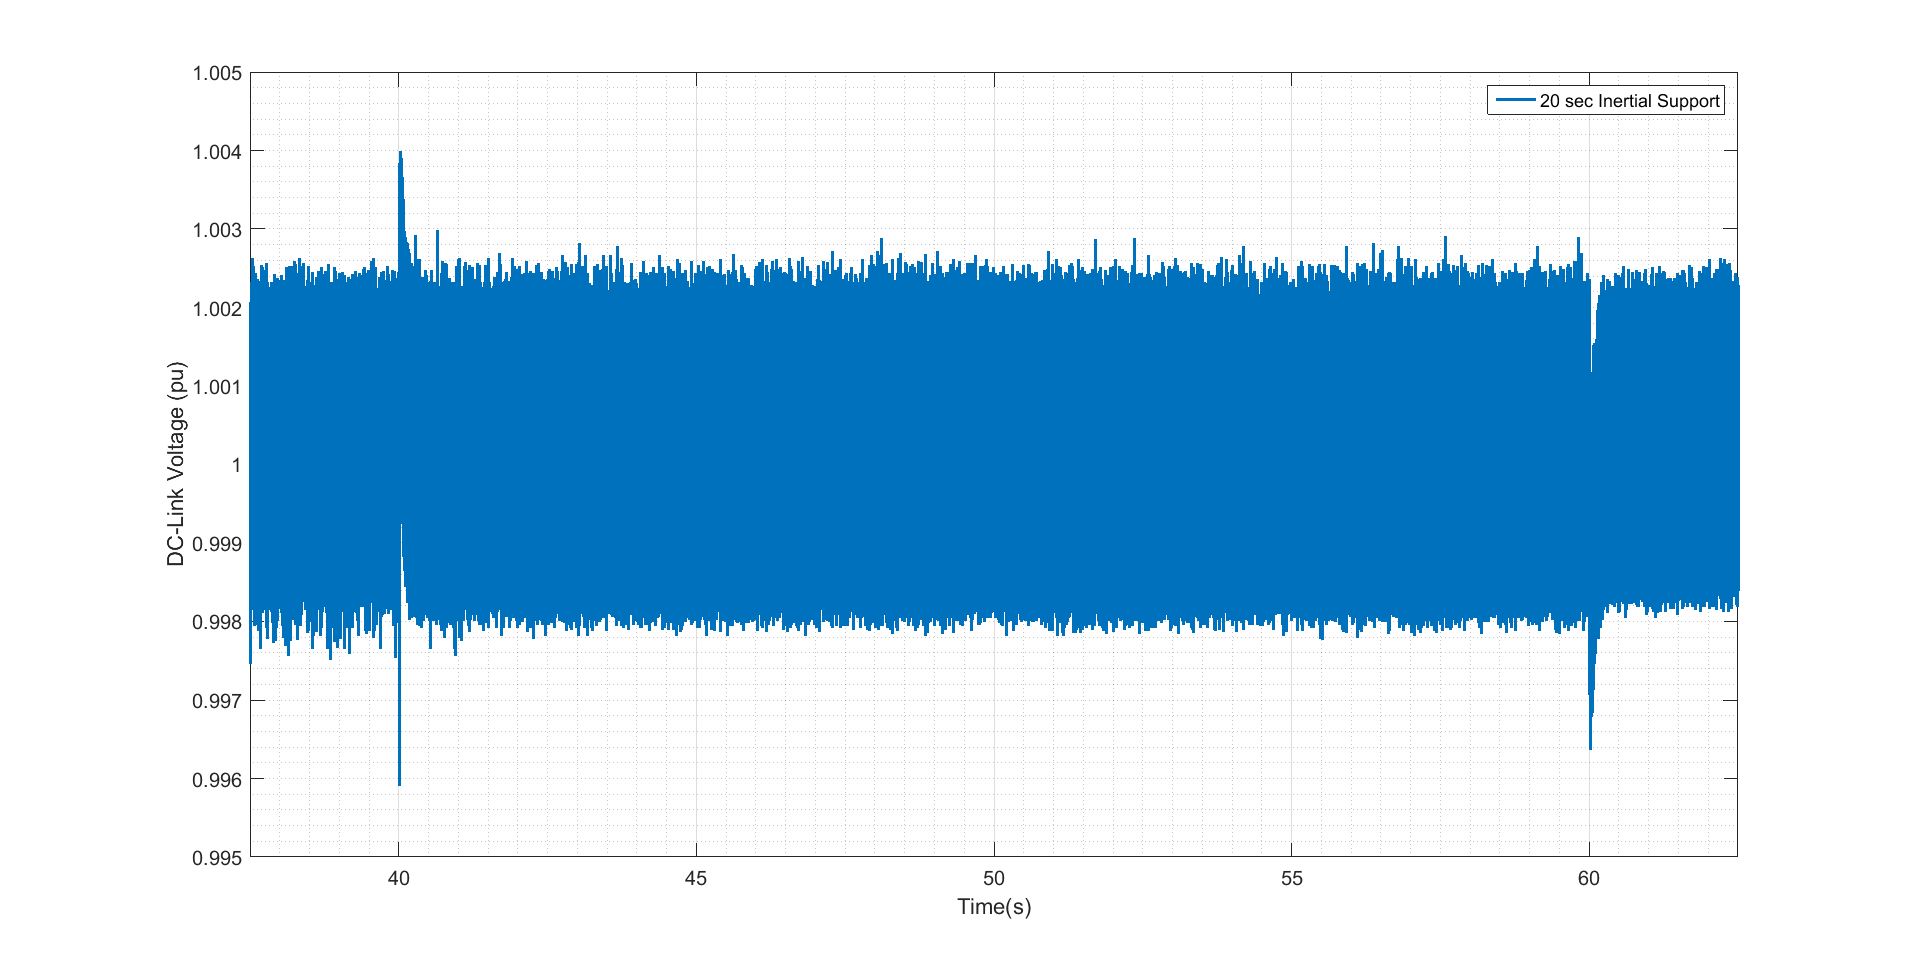
\includegraphics[width=1.0\linewidth]{high_s20_vdc.png}
	\caption{DC-Link Voltage for 20 Seconds Support in High Wind Speed}
	\label{high_s20_vdc}
\end{figure}
% CHAPTER 1
\chapter{EFFECTS OF SYNTHETIC INERTIA IMPLEMENTATION}
\label{chp:5}
The concept of synthetic inertia or virtual inertia suggest a frequency response from renewable energy systems depending on the RoCoF of the electricity grid. As explained at the end of Chapter \ref{chp:3}, a renewable energy system can provide an additional power according to the Swing Equation. In this chapter, the synthetic inertia implementation on a variable speed PMSG wind turbine is tested in P.M. Anderson 9 bus test case which is constructed in Matlab-Simulink environment. The test case is subjected to an sudden load connection in the different scenarios.
\section{P.M.Anderson 9 Bus Test Case}
\subsection{System Properties}
In order to understand frequency dynamics better, P.M. Anderson test case has been used in the study. The single line diagram of the system is given in Fig. \ref{ieee_9_bus}. The test case consists of three generators and three loads. Generators in the system are connected to 230 kV high voltage (HV) network with step-up transformers.\par
The biggest generator in the system is a hydro power plant with a power rating of 247.5 MVA. The remaining ones are steam generators. The power ratings of the generators are given in Table \ref{generatorproperties}.The loads in the system are connected directly to the HV network. The active and reactive power ratings of the loads are listed in Table \ref{loadproperties}. System detailed properties are given in Appendix \ref{chp:appendixB}.
\begin{table}[h]
	\centering
	\begin{tabular}{ccc}
		\hline
		\textbf{Generators} & \textbf{Power Rating (MVA)} & \textbf{Plant Type} \\ \hline
		Gen 1               & 247.5                       & Hydro				\\
		Gen 2               & 192                         & Steam               \\
		Gen 3               & 128                         & Steam               \\ \hline
	\end{tabular}
	\caption{Generator Properties of Test System}
	\label{generatorproperties}
\end{table}
\begin{figure}[h]
	\centering
	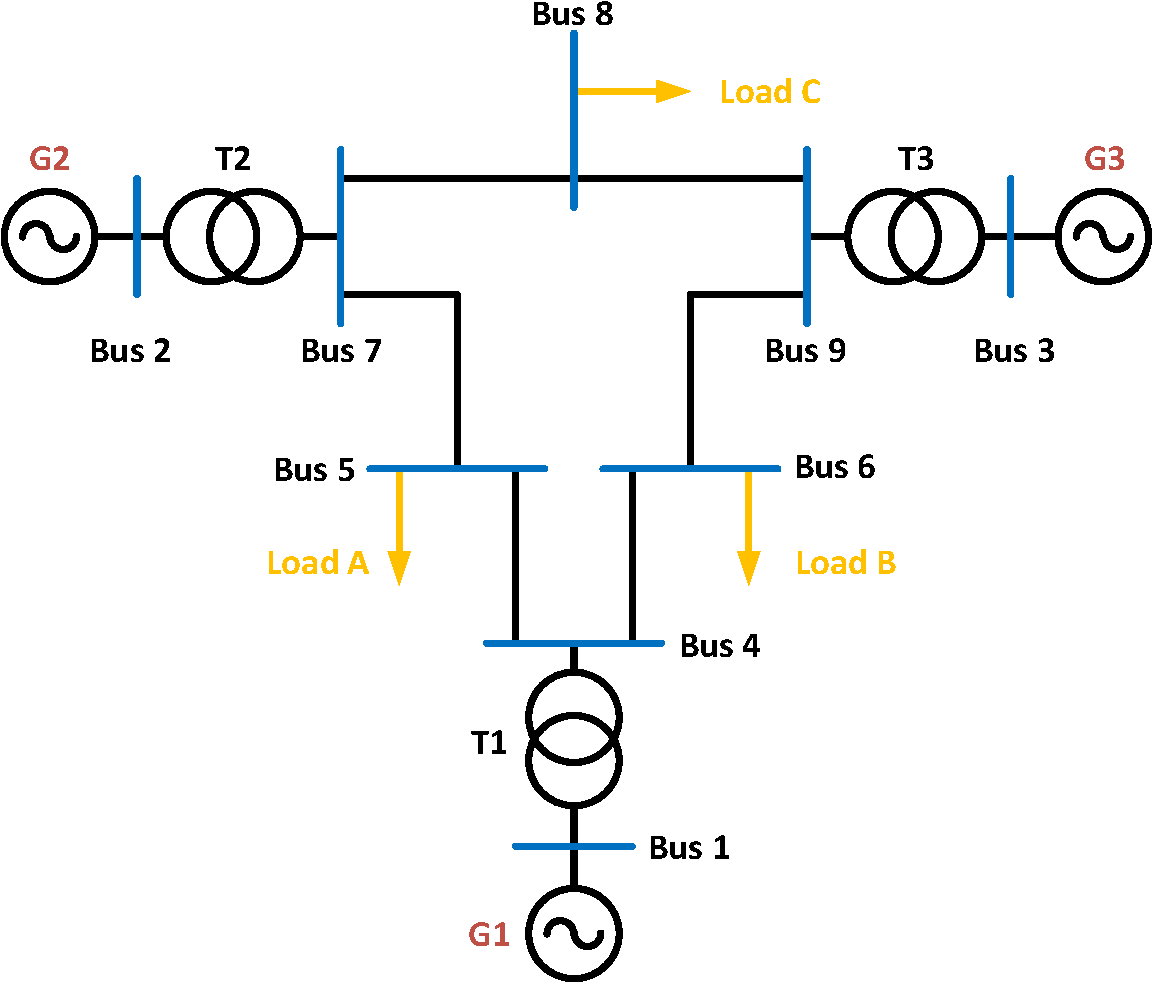
\includegraphics[width=.8\linewidth]{ieee_9_bus.pdf}
	\caption{P.M.Anderson Test Case}
	\label{ieee_9_bus}
\end{figure}
\begin{table}[h!]
	\centering
	\begin{tabular}{ccc}
		\hline
		\textbf{Generators} & \textbf{Active Power (MW)}  & \textbf{Reactive Power (MVAr)} \\ \hline
		Load A              & 125                      	  & 50				 \\
		Load B              & 90                          & 30                \\
		Load C              & 100                         & 35                \\ \hline
	\end{tabular}
	\caption{Load Properties of Test System}
	\label{loadproperties}
\end{table}
\subsection{Load Flow Analysis for Base Case}
Successful grid operation requires a load flow analysis in order to ensure that bus voltages are inside the allowed band and power flows are below the power carrying capabilities of the lines. Load flow results are tabulated in Table \ref{loadflow_case1}.
\begin{table}[h!]
	\centering
	\begin{tabular}{cclccccc}
		\hline
		Bus \# & Bus Type & \multicolumn{1}{c}{Voltage} & Angle & Pg    & Qg     & Pl  & Ql \\ \hline
		1      & SL       & \multicolumn{1}{c}{1.04}    & 0     & 71.65 & 27.05  & 0   & 0  \\
		2      & PV       & \multicolumn{1}{c}{1.025}   & 9.28  & 163   & 6.65   & 0   & 0  \\
		3      & PV       & \multicolumn{1}{c}{1.025}   & 4.66  & 85    & -10.86 & 0   & 0  \\
		4      & PQ       & 1.0258                      & -2.22 & 0     & 0      & 0   & 0  \\
		5      & PQ       & 0.9956                      & -3.99 & 0     & 0      & 125 & 50 \\
		6      & PQ       & 1.0126                      & -3.69 & 0     & 0      & 90  & 30 \\
		7      & PQ       & 1.0258                      & 3.72  & 0     & 0      & 0   & 0  \\
		8      & PQ       & 1.0159                      & 0.73  & 0     & 0      & 100 & 35 \\
		9      & PQ       & 1.0323                      & 1.97  & 0     & 0      & 0   & 0  \\ \hline
	\end{tabular}
	\caption{Load Flow Results in Base Case}
	\label{loadflow_case1}
\end{table}
\subsection{Base Case Frequency Response for Additional Load Connection}
It is obvious that power system networks experience high RoCoF when either high amount of generation trips or high amount of load connects to system. These two main event can be used in the simulation to create frequency disturbances. Since the simulation in Simulink environment slows down with the increasing amount of generators, the disturbances are created with load connections.\par
\begin{table}[h]
	\centering
	\begin{tabular}{ll}
		\hline
		Total System Load                      & 315 MW    \\
		Generator Droop Settings               & 5\%       \\
		Stored Kinetic Energy at Nominal Speed & 3.305 GWs \\
		Gen 1 Inertia Constant                 & 9.5515 s  \\
		Gen 2 Inertia Constant                 & 3.9216 s  \\
		Gen 3 Inertia Constant                 & 2.7665 s  \\ \hline
	\end{tabular}
	\caption{System Dynamical Properties}
	\label{systemdynamicaldata}
\end{table}
System dynamical properties are listed in Table \ref{systemdynamicaldata}. Power generation references are determined based on the load flow of powergui toolbox. Machine initialization toolbox is also used to initiate the state of generators in the system. However, the system does not start with the steady state. Still, system goes to steady state within a few seconds. Frequency of the network is disturbed with a load connection in the t=10 seconds in order to observe the frequency stability of the system. For 10\% load connection, a load of 31.5 MW is connected to system from Bus 6. Location of the additional load is depicted in Fig. \ref{ieee_9_bus_load}.\par
\begin{figure}[h]
	\centering
	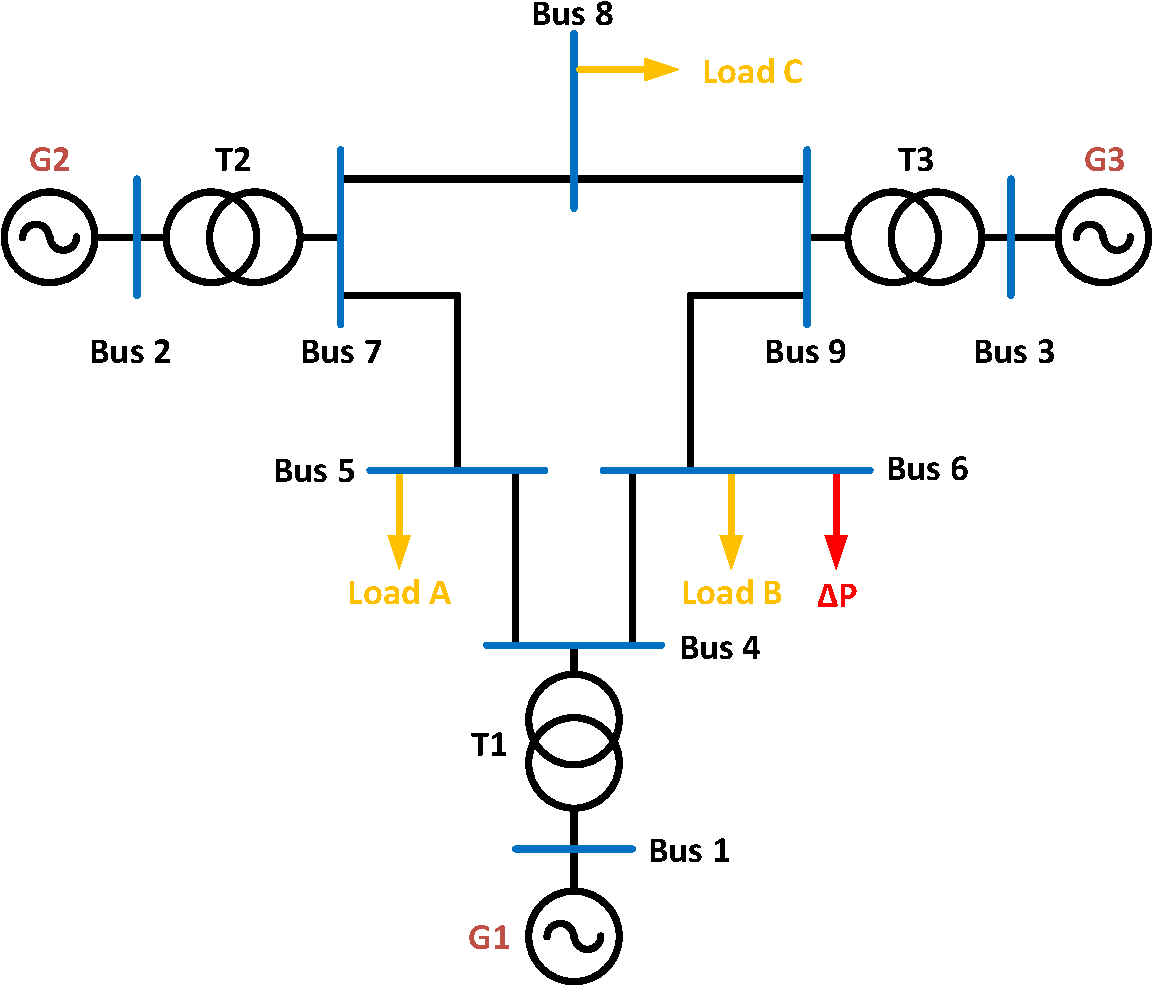
\includegraphics[width=.8\linewidth]{ieee_9_bus_load_position.pdf}
	\caption{Location of the Additional Load}
	\label{ieee_9_bus_load}
\end{figure}
According to the 10\% load connection to system, generator frequencies are shown in Fig. \ref{genfreqcase1}. As it can be seen from Fig. \ref{genfreqcase1}, rotor swings exists in the frequencies. However, the frequency of generator 1 is the most smooth one due to its huge inertia constant. Meanwhile, the generator 2 and generator 3 follow the frequency of generator 1 with higher rotor swings.\par
\begin{figure}[h!]
	\centering
	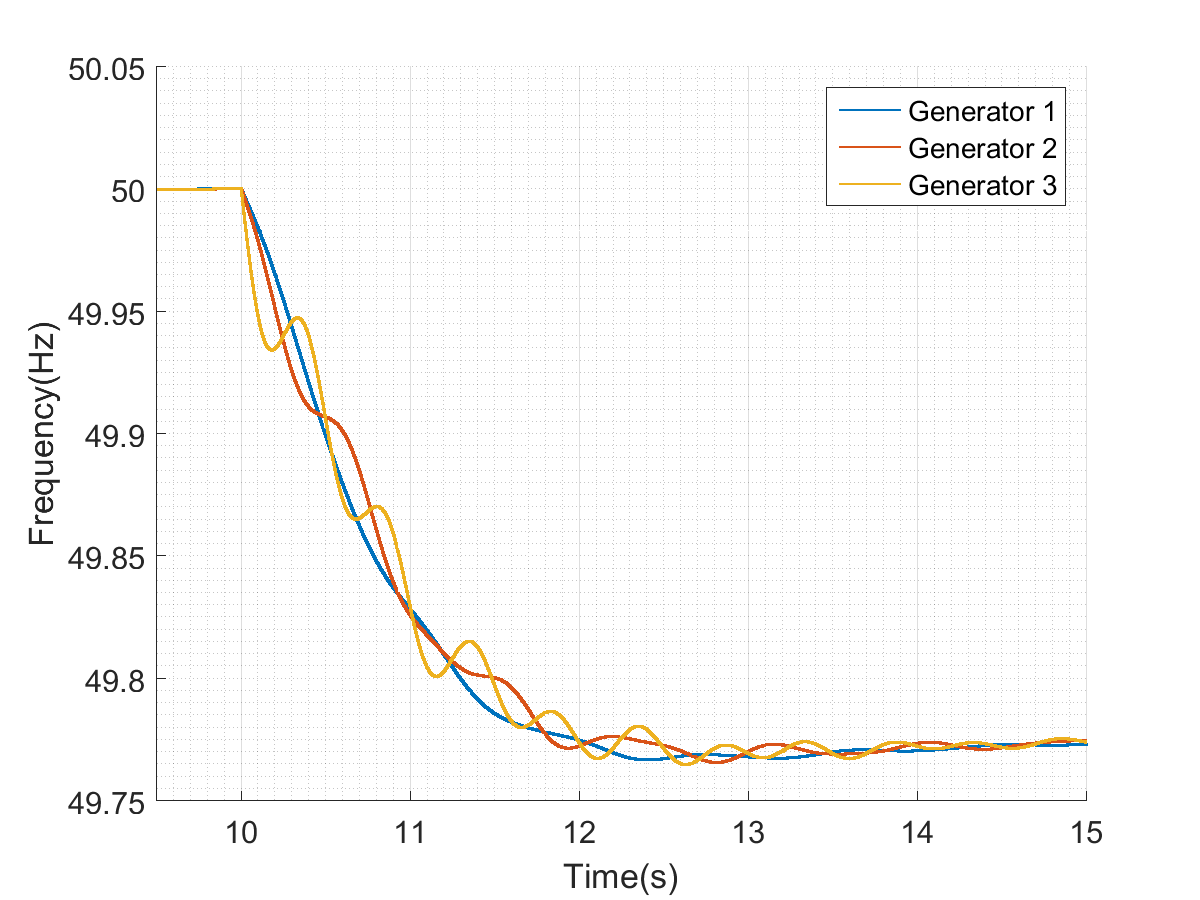
\includegraphics[width=.85\linewidth]{Case1_Generator_Freq.png}
	\caption{Generator Frequencies for 10\% Load Connection}
	\label{genfreqcase1}
\end{figure}
In the system, frequency of Bus 1 can be assumed as constant throughout the network since the system is small enough to assume a single frequency inside the network. This assumption can be verified by comparing the frequencies in Buses 1, 5 and 6. Fig. \ref{genfreqcase1_loadgen} shows the frequency of the generator 1 frequency as well as the load frequencies captured with Simulink PLL block. The only difference is the instant following the load connection. The sharp frequency decline delays the PLL loop to capture the frequency. 
\begin{figure}[h!]
	\centering
	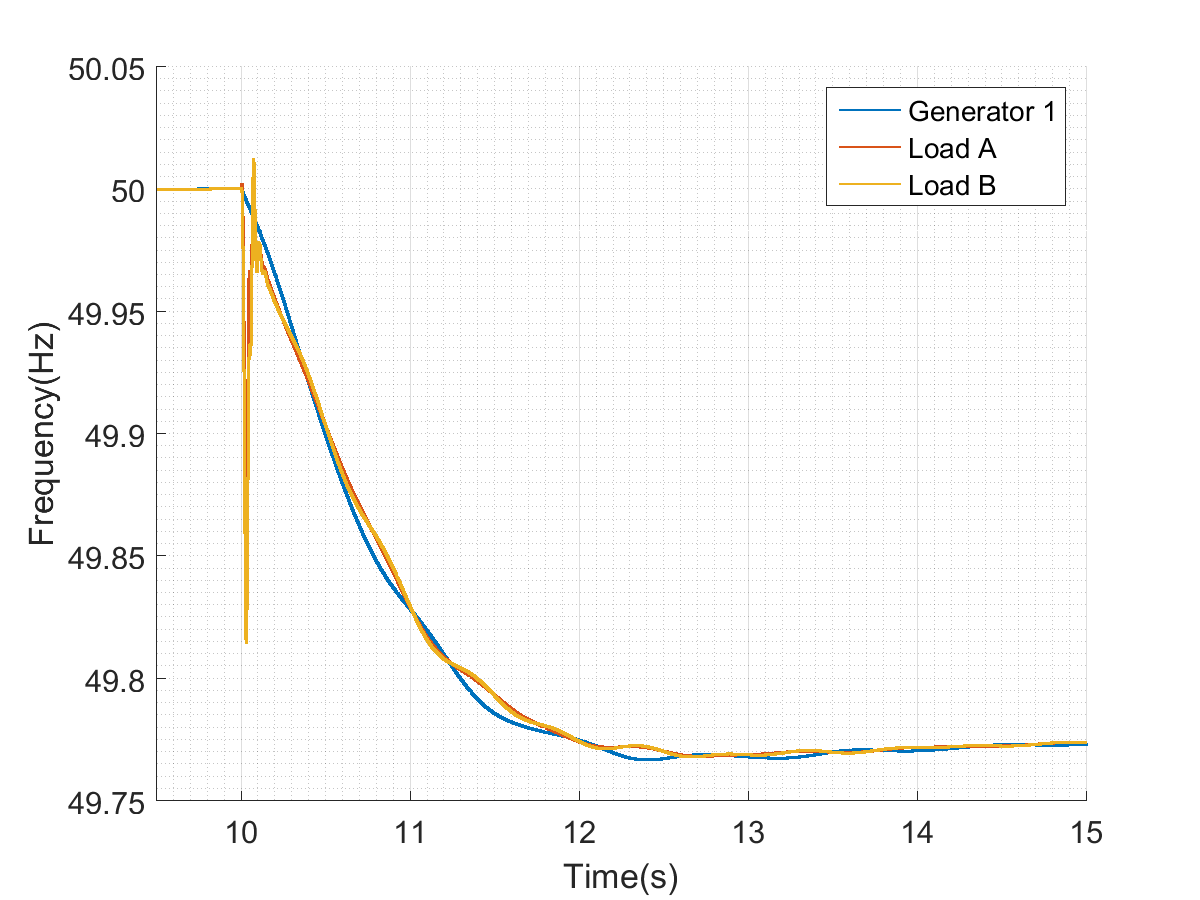
\includegraphics[width=.85\linewidth]{Case1_Load_Gen_Freq.png}
	\caption{Frequencies in Generator 1, Load A and Load B}
	\label{genfreqcase1_loadgen}
\end{figure}
\section{Modified Case}
\label{sec:kmodified}
In order to observe the effect of the renewable energy penetration to grid, the P.M. Anderson test case is modified such that a wind farm consists of 20 wind turbine is connected to network. Since the transmission network of the test case is under-utilized, the location of the wind farm has no effect on the frequency disturbance. Hence bus 5 is selected as the location for wind farm connection. Modified system is depicted in the Fig. \ref{ieee_9_bus_case2}. In this case, generator 2 and 3 are still assigned to same power generation references meanwhile generator 1 decreases its generation since it is the swing generator in the system. 
\begin{figure}[h!]
	\centering
	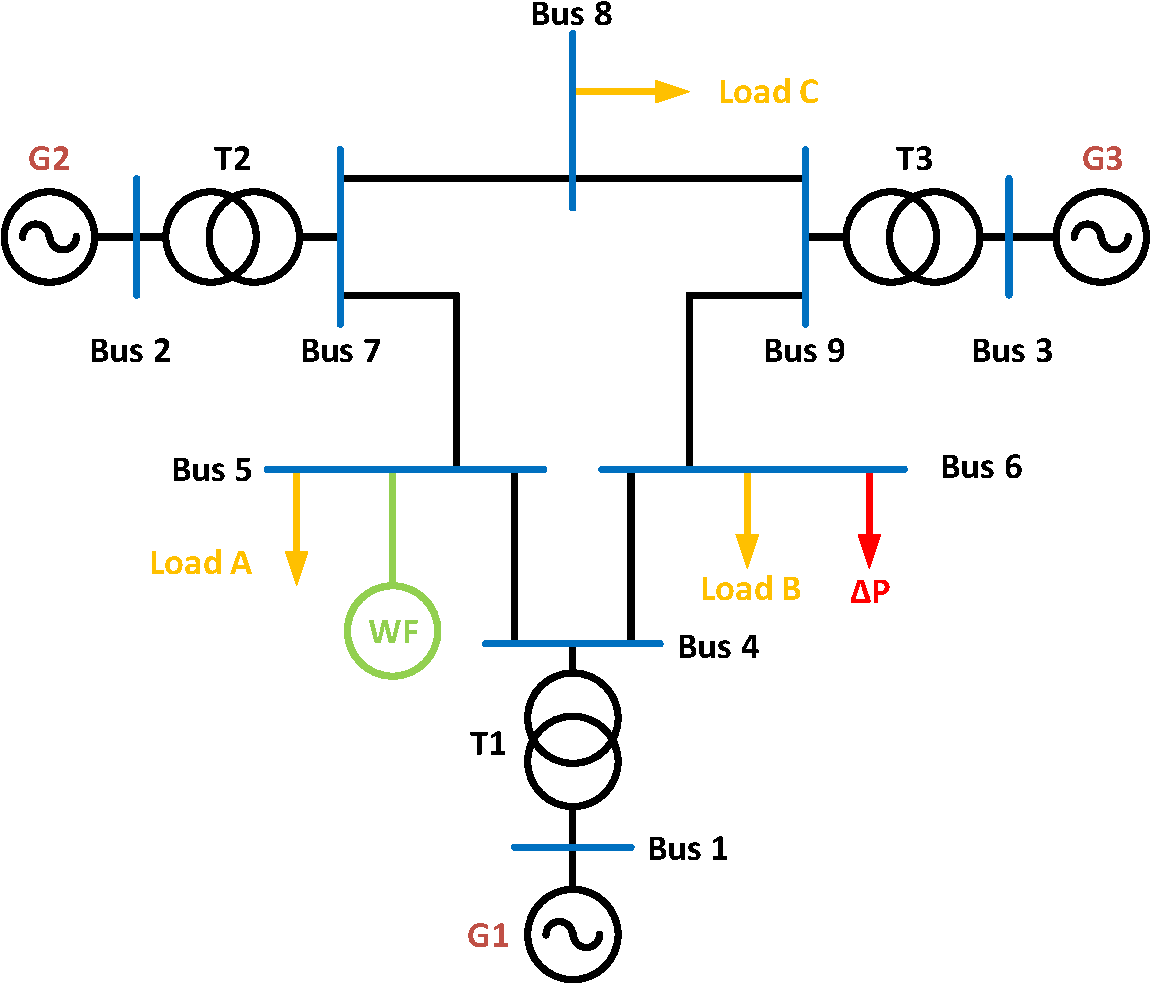
\includegraphics[width=.8\linewidth]{ieee_9_bus_modified.pdf}
	\caption{Modified System Single Line Diagram}
	\label{ieee_9_bus_case2}
\end{figure}
\subsection{Load Flow Analysis for Modified Case}
Load flow analysis for modified case is listed in Table \ref{loadflow_case2}. The power injected from Bus 1 is decreased as expected. This can also be seen from the phase angle between 1 and 4. Phase angle difference between these buses decreased from $2.22^{\circ}$ to $1.18^{\circ}$. Total power generation from active power from conventional generation units are also decreased. Therefore, the modified system resembles the base case with low power demand.
\begin{table}[h!]
	\centering
	\begin{tabular}{cclccccc}
		\hline
		Bus \# & Bus Type & \multicolumn{1}{c}{Voltage} & Angle & Pg    & Qg     & Pl  & Ql \\ \hline
		1      & SL       & \multicolumn{1}{c}{1.04}    & 0     & 38.06 & 25.07  & 0   & 0  \\
		2      & PV       & \multicolumn{1}{c}{1.025}   & 11.33 & 163   & 6.65   & 0   & 0  \\
		3      & PV       & \multicolumn{1}{c}{1.025}   & 6.32  & 85    & -10.86 & 0   & 0  \\
		4      & PQ       & 1.0263                      & -1.18 & 0     & 0      & 0   & 0  \\
		5      & PQ       & 0.9995                      & -1.54 & 0     & 0      & 125 & 50 \\
		6      & PQ       & 1.0128                      & -2.43 & 0     & 0      & 90  & 30 \\
		7      & PQ       & 1.0266                      & 5.77  & 0     & 0      & 0   & 0  \\
		8      & PQ       & 1.0164                      & 2.62  & 0     & 0      & 100 & 35 \\
		9      & PQ       & 1.0326                      & 3.62  & 0     & 0      & 0   & 0  \\ \hline
	\end{tabular}
	\caption{Load Flow Results for Modified Case}
	\label{loadflow_case2}
\end{table}
\subsection{Modified Case Frequency Response for Additional Load Connection}
The modified base is very similar to the Base Case except for a wind farm located in Bus 5. The renewable energy system in this case can be considered as a negative load. Therefore, base case with decreased load is under discussion in this subsection. The same amount of load is taken into operation at Bus 6 and the frequency response of the modified system is shown in Fig. \ref{Case1_2_freq}. \par
\begin{figure}[h!]
	\centering
	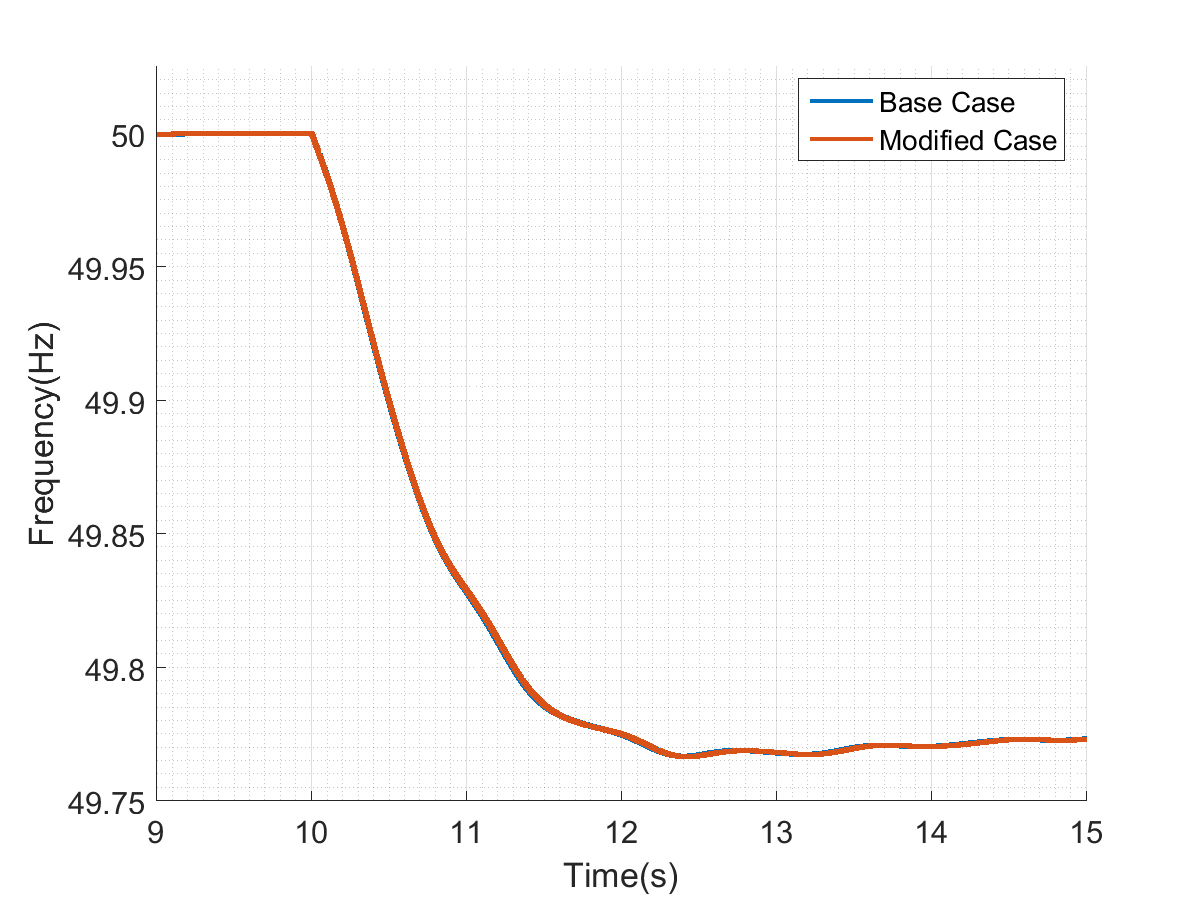
\includegraphics[width=.85\linewidth]{Case1_2.png}
	\caption{Comparison of Base Case and Modified Case Frequencies}
	\label{Case1_2_freq}
\end{figure}
Almost the same frequency response is observed in the system. The reason is that both systems have the same amount of stored kinetic energy. Another reason is that there is no congestion in the system due to under-utilized of transmission network. The same frequency response can also be observed in the rate of change of frequencies in Fig. \ref{Case1_2_rocof}. Almost the same RoCoF values are observed in the system. This concludes that renewable energy penetration does not change frequency response of the system if the only change in the system is the inclusion of renewable energy system. In other words, renewable energy systems does not affect the frequency response of the grid unless the system is replaced with a conventional generation unit. Note that the renewable energy systems are intermittent energy sources. However, in this study,the source of the renewable energy system is assumed as constant. Therefore, the reason of frequency disturbance is load connection rather than the change in active power output of renewable systems.
\begin{figure}[h!]
	\centering
	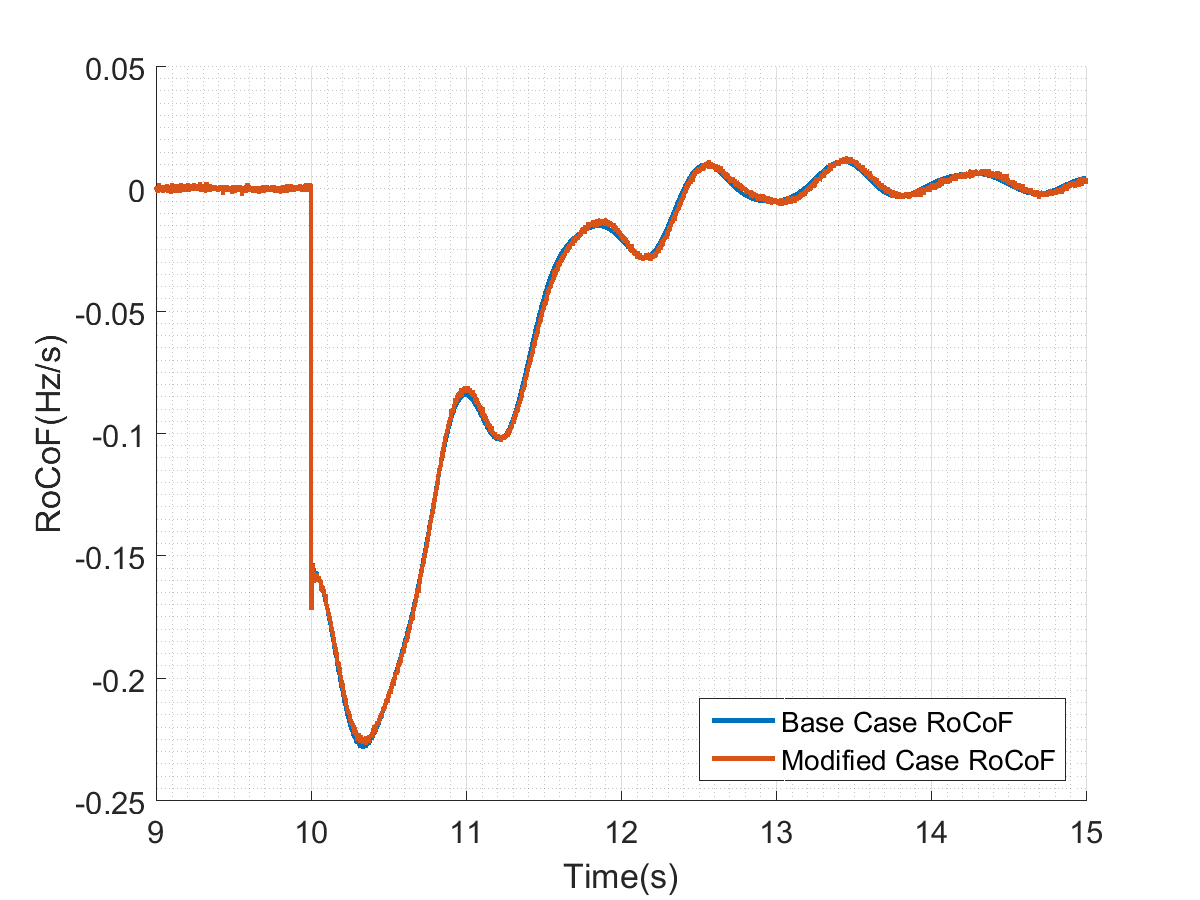
\includegraphics[width=.85\linewidth]{Case1_2_rocof.png}
	\caption{Comparison of Base Case and Modified Case Frequencies}
	\label{Case1_2_rocof}
\end{figure}
\section{Decommissioned Case}
\label{sec:kdecommissioned}
As seen in the Modified Case, the frequency response of the system does not change with renewable energy inclusion. However, it is inevitable that renewable energy systems will replace the conventional units in future. In this case, the smallest generator, generator 3, will be decommissioned due to economical concerns. The decommissioned case diagram is shown in Fig. \ref{decommissioned_case}.\par
\begin{figure}[h!]
	\centering
	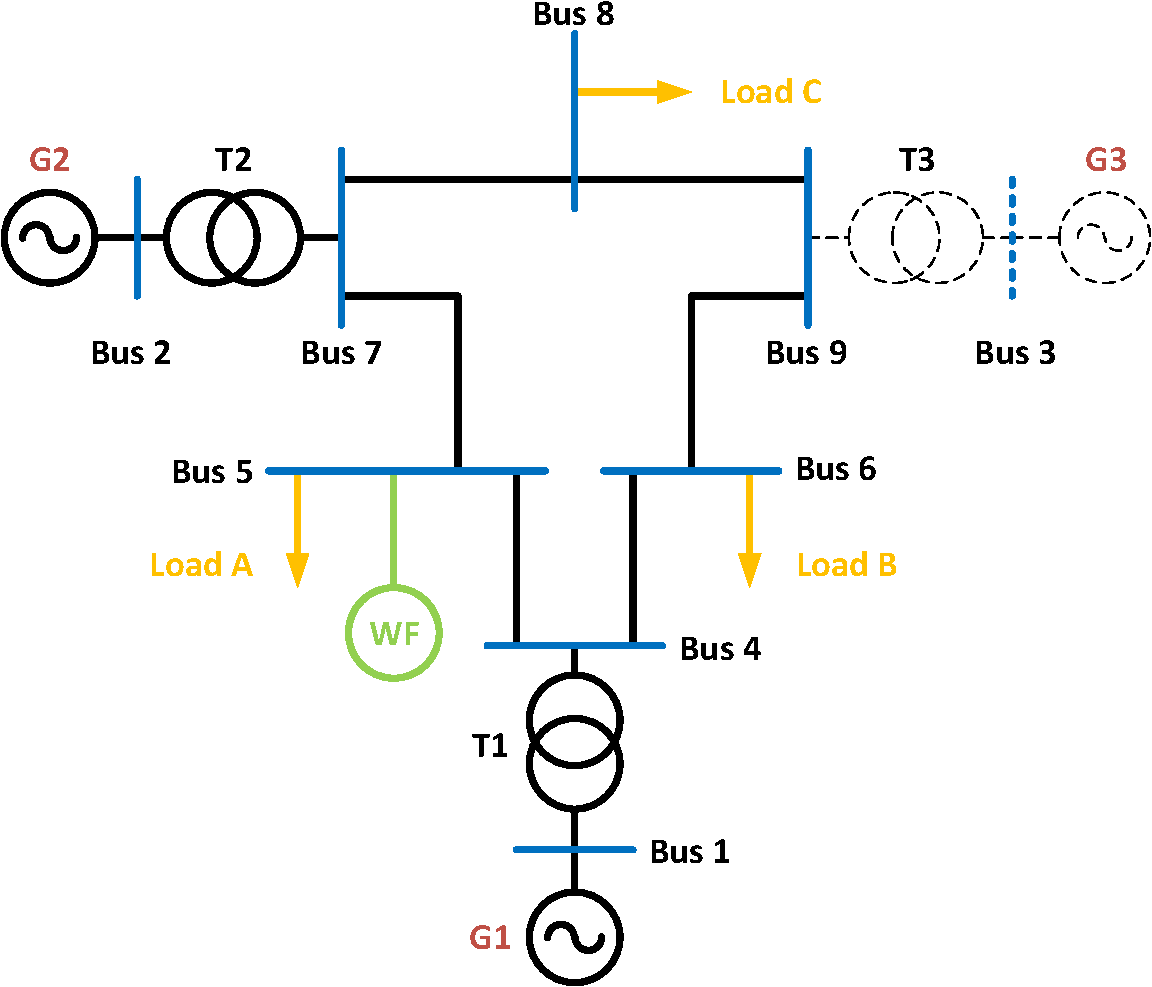
\includegraphics[width=.8\linewidth]{ieee_9_bus_decommissioned.pdf}
	\caption{Decommissioned Case Sinle Line Diagram}
	\label{decommissioned_case}
\end{figure}
Since the generator 3 is out of service, the stored kinetic energy is decreased in the system. Decommissioned system dynamical properties are updated and given in Table \ref{systemdynamicaldatacase3}. Higher RoCoF value and lower frequency nadir are expected with the same additional load since the system dynamical properties are deteriorated with the removal of generator 3.
\begin{table}[h]
	\centering
	\begin{tabular}{ll}
		\hline
		Total System Load                      & 315 MW    \\
		Generator Droop Settings               & 5\%       \\
		Stored Kinetic Energy at Nominal Speed & 3.004 GWs \\
		Gen 1 Inertia Constant                 & 9.5515 s  \\
		Gen 2 Inertia Constant                 & 3.9216 s  \\
		\hline
	\end{tabular}
	\caption{System Dynamical Properties}
	\label{systemdynamicaldatacase3}
\end{table}
\subsection{Load Flow Analysis for Decommissioned Case}
Since the generator 3 is out of service, generator 1 loading will be increased. Load flow analysis for decommissioned case is given in Table \ref{loadflow_case3}.
\begin{table}[h!]
	\centering
	\begin{tabular}{cclccccc}
		\hline
		Bus \# & Bus Type & \multicolumn{1}{c}{Voltage} & Angle & Pg    & Qg     & Pl  & Ql \\ \hline
		1      & SL       & \multicolumn{1}{c}{1.04}    & 0     & 121.76& 16.26  & 0   & 0  \\
		2      & PV       & \multicolumn{1}{c}{1.025}   & 4.18  & 163   & 0.65   & 0   & 0  \\
		4      & PQ       & 1.0332                      & -3.74 & 0     & 0      & 0   & 0  \\
		5      & PQ       & 1.0083                      & -5.63 & 0     & 0      & 125 & 50 \\
		6      & PQ       & 1.0224                      & -7.65 & 0     & 0      & 90  & 30 \\
		7      & PQ       & 1.0294                      & -1.36 & 0     & 0      & 0   & 0  \\
		8      & PQ       & 1.0207                      & -5.82 & 0     & 0      & 100 & 35 \\
 \hline
	\end{tabular}
	\caption{Load Flow Results for Decommissioned Case}
	\label{loadflow_case3}
\end{table}
\subsection{Decommissioned Case Frequency Response for Additional Load Connection}
Decommissioned system is also subjected to the same frequency disturbance which is the additional load connection from Bus 6. System frequency response is observed and compared to Base Case and Modified Case in Fig. \ref{Case1_2_3_freq}. The frequency response of the system gets worse with the generator 3 decommissioned. It results that the frequency nadir is decrease from 49.77Hz to 49.65Hz due to the decrease in the stored kinetic energy in the system. The deteriorated frequency response can also be seen from the comparison of RoCoFs that is given in Fig. \ref{Case1_2_3_rocof}. 
\begin{figure}[h]
	\centering
	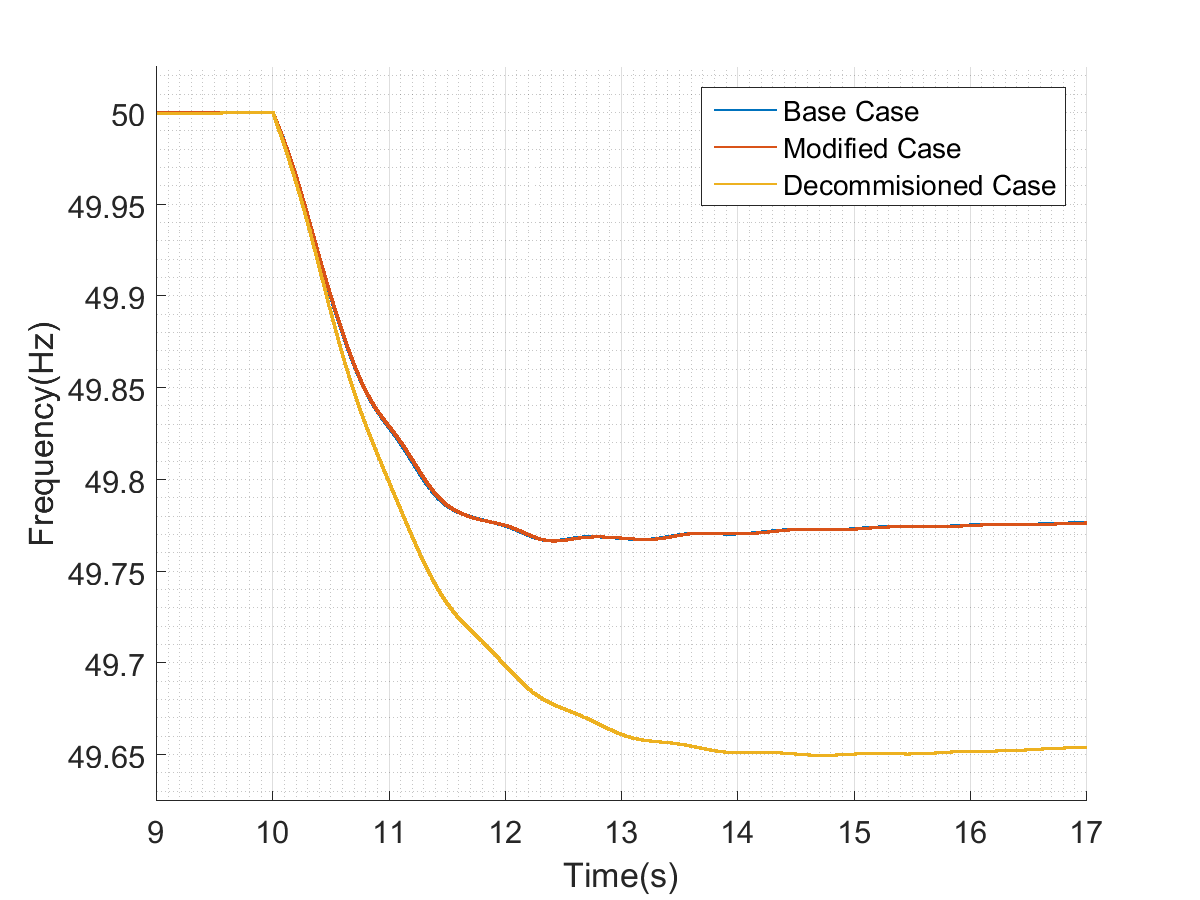
\includegraphics[width=.85\linewidth]{Case1_2_3_freq.png}
	\caption{Comparison of Base Case,Modified Case and Decommissioned Case Frequency Responses}
	\label{Case1_2_3_freq}
\end{figure}
\begin{figure}[h]
	\centering
	\includegraphics[width=.85\linewidth]{Case1_2_3_rocof.png}
	\caption{Comparison of Base Case,Modified Case and Decommissioned Case RoCoFs}
	\label{Case1_2_3_rocof}
\end{figure}
\section{Modified Case with Synthetic Inertia}
The frequency response of the modified system is investigated in Section \ref{sec:kmodified} and the system frequency was almost the same with test system base case. However, the response of the system can be improved by provision of synthetic inertia. The wind turbines in the system is equipped with synthetic inertia that emulates inertia constants of 5s, 10s and 15s. The system response with inertial support provision is given in the Fig. \ref{Case4_freq}.\par
\begin{figure}[h!]
	\centering
	\includegraphics[width=.9\linewidth]{case4_frequencies.png}
	\caption{Emulation of the Different Inertia Constants for the Modified Case}
	\label{Case4_freq}
\end{figure}
Since the modified case frequency response is almost the same with the base case, the synthetic inertia implementation is improved the system frequency response. In other words, the wind turbines are integrated to the system by emulating the synchronous generator behaviour. It is to note that huge amount of kinetic energy exists in the wind turbine systems. That stored energy can be utilized with the synthetic inertia method in order to improve frequency dynamics of the system.\par
Emulation of synchronous generator behaviour is basically increasing the amount of active power depending on the RoCoF of the grid and the inertia constant to be emulated. Since the higher inertia constant requires higher active power increase, the inertia constants of 10s and 15s result in better frequency dynamics. The frequency nadir of the base case is slightly increased. The effect of the synthetic inertia provision can also be observed in the system RoCoF values that is given in Fig. \ref{Case4_rocof}.\par
\begin{figure}[h]
	\centering
	\includegraphics[width=1\linewidth]{case4_rocof.png}
	\caption{RoCoF of the Different Inertia Constants for the Modified Case}
	\label{Case4_rocof}
\end{figure}
It is obvious that the base case experience the highest RoCoF in the very first second of the frequency disturbance. While the remaining cases is subjected to lower RoCoF at first, the base case RoCoF is the lowest following seconds. The reason is that the base case active power contribution in the first second is much higher than others. Hence, the case subjected to severe conditions react higher and faster resulting quick restoration of the system. Another observation is that all cases converges to the same steady state frequency due to the fact that inertial support affects the transient rather than the steady state values. The steady state frequency is dependent on the capacity of conventional synchronous generators and their droop constants. This is why the decommissioned case steady state frequency is lower than that of modified case.
\section{Decommissioned Case with Synthetic Inertia}
Decommissioned case frequency response for 10\% additional load connection is studied in the Section \ref{sec:kdecommissioned}. System frequency experiences high RoCoF and lower steady state frequency because of the removal of the generator 3. In this section, synthetic inertia method  is implemented on the decommissioned case wind farm with different inertia constants. The resultant frequency responses are shown in the Fig. \ref{Case5_freq}. As in the case of modified case, base case frequency response experiences steepest decline in the frequency meanwhile the higher inertia constant synthetic inertia implementations have smoother frequency decrease.\par
\begin{figure}[h]
	\centering
	\includegraphics[width=0.9\linewidth]{case5_frequency.png}
	\caption{RoCoF of the Different Inertia Constants for the Decommissioned Case}
	\label{Case5_freq}
\end{figure}
The active power of the wind turbine for the different inertia constants is given in Fig. \ref{Case5_power}. It should be noted that the active power of the wind turbine is proportional with the RoCoF that is also given in Fig. \ref{Case5_rocof}. Note that 15s inertia constant is also emulated. It is stated that conventional generator inertia constants lie between 2-9s \cite{Kundur}. Nonetheless, synchronous generators have constant kinetic energy in the nominal frequency. However, the kinetic energy stored in the turbine inertia fluctuates with the generator speed. Moreover, wind turbine is able to emulate different inertia constant as soon as it has the capacity to increase its power. Even with the inertia constant of 15s, the wind turbine is far away from its maximum allowable power. Therefore, higher inertia constants can also be tested in the expense of longer speed recovery process whose resultant decreased power might also affect the RoCoF further. 
\begin{figure}[h]
	\centering
	\includegraphics[width=0.9\linewidth]{case5_powers.png}
	\caption{Wind Turbine Active Power for the Different Inertia Constants in the Decommissioned Case}
	\label{Case5_power}
\end{figure}
\begin{figure}[h!]
	\centering
	\includegraphics[width=0.9\linewidth]{case5_rocof.png}
	\caption{Wind Turbine Active Power for the Different Inertia Constants in the Decommissioned Case}
	\label{Case5_rocof}
\end{figure}
\section{Comparison of the Synthetic Inertia and Fast Inertial Support}
In the Chapter \ref{chp:4}, it is stated that the wind turbines have more than sufficient capacity in order to increase its active power. The fast inertial support concept is studied with different increase rates. The exaggerated inertial supports are studied to observe the turbine internal dynamics. In this section, the fast inertial support will be compared with the synthetic inertia. In other words, increasing active power by a defined percentage will be compared to a rise in the active power proportional to RoCoF. For this reason, the same frequency disturbance is tested on the base case decommissioned case, the case where inertia constant of 10s is emulated and also the one with fast inertial support with 5\% increased power by 5 seconds. Fig. \ref{Comp_power} shows the variation of the active power. In order to increase the effectiveness of the fast inertial support, it is activated with a delay of 0.25s. In this interval, the synchronous generators take action for the upcoming disturbance. It should be underlined that the active power of the inertia emulated case is increased proportional to the RoCoF. Therefore, it declines as the RoCoF declines. Therefore, in the other half of the support time, it is below of the fast inertial support case. This phenomena can be clearly observed in the frequency response. It should be underlined that the swing equation is also used in fast inertial support recovery process in order to smooth recovery. This is why the active power of the both methods are the same in the recovery.\par
\begin{figure}[h]
	\centering
	\includegraphics[width=0.9\linewidth]{comparison_power.png}
	\caption{Comparison of the Frequency Responses for the Base, Fast Inertial Support and Synthetic Inertia Cases}
	\label{Comp_power}
\end{figure}
The frequency response of these three cases is shown in Fig. \ref{Comp_freq}. It is obvious that the base case frequency response has the poorest transient frequency. Besides, the synthetic inertia implemented case has the best transient behaviour for the very first seconds. Nonetheless, the fast inertial support case first converges to higher steady state frequency until the end of the support period. However, as soon as the support ends, the sharp decrease in the active power results a second dip in the frequency. The decrease in the active power can be considered as a second load connection to system. Therefore, the frequency is exposed to a second decrease at the end of support period in fast inertial support implementation. In contrary, the synthetic inertia case active power is decreased down to lower values as the RoCoF is positive. Than means that the recovery process is already started inside the support. Hence, the secondary dip is not observed in this case. \par
\begin{figure}[h!]
	\centering
	\includegraphics[width=0.9\linewidth]{comparison_freq.png}
	\caption{Comparison of the Active Power Increase in Fast Inertial Support Case and Synthetic Inertia Case}
	\label{Comp_freq}
\end{figure}
Finally, it should be noted that the energy extracted from wind turbine in the first 4 seconds are the same for both methods. However, synthetic inertia support utilizes that energy better by distributing the energy according to the RoCoF. Therefore, the grid takes the highest energy when it is needed most. But, the fast inertial support gives the same amount of energy for the support time. Besides, the additional power is cut suddenly that ruins the support. Hence, the fast inertial support needs to decrease the distribution of this energy according to some algorithms whose development is also out of scope of this study.
% CHAPTER 1
\chapter{EVALUATION OF FAST INERTIAL RESPONSE AND SYNTHETIC INERTIA IMPLEMENTATION}
\label{chp:6}
Increase in share of renewable energy in the installed capacity brought operational problems. Due to the fact that PV systems do not have rotational mass at all or wind turbines with full-scale or partial scale power electronics do not effectively contribute the grid aggregated inertia, the power system with increasing renewable energy penetration will be exposed to high RoCoF for the frequency disturbances. This implies that system will encounter unacceptable RoCoF values (around the RoCoF protection settings of the generating units) in the normal operation as long as the renewable penetration continues. Therefore, the upcoming future power system will require auxiliary services such as synthetic i.e. virtual inertial support from all generation technologies that includes power electronics. \par
Renewable energy systems produces power according to the type of its power source. The input power is constant for an instant since the source (solar radiation, wind speed etc.) is constant. Therefore, the operation of renewable systems is different from the conventional power plants in which input power can be controlled by the operator. Nonetheless, an additional energy source is required in the renewable systems in order to increase active power as desired. For this purpose, rotational kinetic energy in wind turbine blades and generator can be utilized. In this way, the wind turbines are able to increase their active output power by extracting the kinetic energy stored in the turbine equivalent inertia. However, the amount of active power increase can be either constant as in the case of Chapter \ref{chp:4} or dynamic (proportional to RoCoF) as in the case of Chapter \ref{chp:5}.
\section{Fast Inertial Support}
Wind turbines with full-scale power electronics can adjust its active power by controlling its output torque. Therefore, the active power can be quickly raised by extracting the stored energy in the turbine inertia. However, the maximum value of the active power that can be extracted depends on the operating conditions. Since the generator active power is also dependent on its speed, turbine power cannot be increased up to rated power but to half of the rated power in wind speeds lower than 5m/s. In wind speeds higher than 10m/s, the active power before the support is already close to its rated value. Therefore, the increase in the active power is limited as 10\% (as long as converter rating has the capacity) in high wind scenarios. \par
In this study, the wind turbine can increase its active output power by 1.2MW in the wind speeds between 5m/s and 8m/s for fast inertial response. The highest active power release is found in the wind speed 6.5m/s as 1.3MW. Besides, wind turbines can contribute better in low wind scenarios than that of high wind speed for short time intervals. However, when the active power increase is limited with 10\%, \par
It should be noted that the frequency disturbance occurs due to the unbalance between input mechanical power and output powers of the generators. Hence, the additional amount of active power that is provided from renewable energy sources in such instants is favourable. This is why the amount of increase in the active power is important. Therefore, knowledge of active power limits reveals the potential of wind turbines with FSPC in order to contribute the frequency stability of the power systems.\par
Fast inertial response can be provided within different time durations up to 30 seconds. Since the larger amount of support might result in higher speed deviations, the support time might be decreased. In contrary, higher support durations can be achieved with lower amount of fast inertial response. Notice that turbine will decrease its output power after the support period to restore its speed. Therefore, the additional energy will be the zero at the end of the support. \par
Fast inertial response in this study is not a direct function of the RoCoF. In other words, the support power is independent from RoCoF or frequency deviation. However, the activation of the support is based on a RoCoF threshold of 0.1Hz/s with the frequency dead-band 10mHz. A RoCoF indexing can be developed to obtain different support power values. In this case, the indexing scheme requires a RoCoF threshold and different RoCoF intervals. The highest RoCoF interval corresponds to the most severe frequency disturbances case (RoCoF above 0.5Hz/s) and requires the highest amount of fast inertial support release with highest available support time. Meanwhile, the lowest RoCoF interval would be assigned to lowest inertial support release with time duration in order not to result higher speed deviation. It should be noted that the higher energy extraction might even result in the stall of the turbine. Nonetheless, critical instant following the disturbance is much more important than the turbine speed recovery. Hence, grid operators might choose to extract the available active power in the expense of turbine stall according to the optimized decision.
\section{Synthetic Inertia Implementation}
Even though wind turbine power can be increased as desired between 0.1pu and 0.45pu range by using fast inertial support, the fastest release of the power independent of the frequency is not the best solution especially for weak power grids. Although additional amount of power is released in the disturbances, the restoration of the energy to the turbine causes might create a second frequency decrease in the grid. Therefore, the increase amount should be in coordination with the grid frequency behavior. This is why dynamic frequency response is obtained with the synthetic inertia implementation in the Chapter \ref{chp:5}. \par
By adjusting active power according to the RoCoF of the grid, the active power is increased or decreased depending on the grid status. If the frequency decreases, additional amount of active power proportional to RoCoF will be injected to grid. The advantage of the dynamic frequency response is the fact that the active power is decreased below the pre-disturbance power value as grid RoCoF is positive. This implies that the restoration of the turbine speed begins with positive RoCoF avoiding a second drop in the frequency.\par
In order to observe the effects of synthetic inertia implementation, a dynamical 9-bus test system is constructed in Matlab-Simulink environment. The test system is composed of the conventional generators and subjected to a frequency disturbance with a load connection. In order to see the effects of the renewable energy penetration, a wind farm with 20 turbines is connected to system. In the 10\% Renewable Case, the system frequency behavior is not affected from the renewable penetration. The maximum RoCoF of 0.23Hz/s is observed in the system. The maximum RoCoF decreased down to 0.25Hz/s in the Reduced Inertia Case. The frequency behavior is improved by the synthetic inertia by lowering the RoCoF values down to 0.19Hz/s in 10\% Renewable Case and 0.21Hz/s in the Reduced Inertia Case.
\par
The most important feature of the synthetic inertia implementation is the RoCoF dependency. The inertial support in this method does decrease the active power as soon as RoCoF turns positive meaning that turbine speed recovery can be started. Thus, the speed recovery of the synthetic inertia method begins when the frequency nadir is reached.\par
The synthetic inertia implementation is used for improving the transient behavior of the frequency. In the literature, variety of inertia constants are emulated in variable speed wind turbines between the inertia constant up to 10 seconds \cite{Gonzalez-Longatt2013},\cite{Gonzalez-Longatt}. Chapter \ref{chp:4} demonstrates that the wind turbines are able to increase its active power temporarily by 0.45pu. In this study inertia constants more than 10 seconds are also tested. Nonetheless, the inertia constants more than 10s is not possible in the high wind speed range. Nonetheless, inertia constant of 10s is applicable for whole speed range. Inertia constants above 10s can also be achievable as long as the converter rating is available. In the worst case scenario, output power saturates to the limit for a part of the support duration. However, as the RoCoF decreases, output power can follow the commanded output power.\par 
Synthetic inertia implementation in the Turkish electricity network is also evaluated based on the hourly generation data from 2018. The effect of the varying generation profile is calculated by considering wind and solar energy. It is shown that the decrease in the aggregated inertia constant of the grid can be compensated with the help of synthetic inertia implementation to wind turbines with FSPC. In fact, the wind turbines with FSPC are able to compensate not only the decrease due to their existing structure but also the decrease due to other wind turbines (DFIG and Type I-II) and PV systems. This is why the synthetic inertia should be implemented in all of the wind turbines with full-scale power converter.
\section{Economical Motivations for Energy Providers}
As explained in Section \ref{section-price}, renewable energy systems in Turkey and most of the EU countries sell electricity with feed-in tariff. It basically means that all the generated energy is sold without trading in day-ahead market. Even though the problems are arising with renewable energy systems, the energy providers would not be a volunteer for ancillary services unless the regulations impose sanctions or additional payment is provided to turbine owners. Hence, the system operator should prepare more advantageous compensation mechanisms in order to convince energy providers to implement grid supporting methods. \par
The system operators has already started preparing new frequency regulations. One of the examples is the Firm Frequency Response (FFR) by National Grid \cite{NationalGridElectricityTransmission2016}. FFR is basically frequency support method that is activated with the frequency thresholds. As the frequency falls below a pre-determined value, a response is required by the energy providers (either from synchronous generators or energy storage units). These energy providers are taken into operation according to their bids. The response is either non-dynamic (independent from the frequency shift) or dynamic (pre-determined percentage increased according to frequency). Moreover, the support power should be sustained up to 30 seconds dynamic response and up to 30 minutes for non-dynamic response for the primary \cite{Smethurst2017}. This is why the response is provided by synchronous generators and energy storage systems in which active power output can be adjusted as desired. It should be noted that this mechanism is not appropriate for the renewable energy systems where the output power can be increased up to 30 seconds by utilizing the stored energy in the inertia or DC-link capacitor.\par
Another frequency regulating mechanism is applied in USA according to the FERC 755 regulation \cite{FederalEnergyRegulatoryCommission2011}. The frequency regulation includes different metrics for payment such as capacity, performance and mileage. Based on this regulation, energy price for the high performance frequency regulation resources is increased over three times of the old price of the PJM which is a regional transmission company \cite{NECEnergySolutions2014}. Since one of the metrics effecting the payment is performance, the regulation is advantageous for energy storage systems that can adjust its active power quickly thanks to their power electronics interface.\par
When the wind turbine is used for inertial support mechanisms, additional power up to 0.45pu can be achieved for 3s or 0.1pu power with unlimited duration (as long as converter can handle). The longer time durations might cause problems for power converter such as heating. Even though the turbine injects significant amount of power to grid, the additional amount of energy (4000KWs) is negligible compared to daily energy production. Therefore, the payment for the additional amount of energy would not be beneficial to energy provider. \par
In order to investigate the economical side of the frequency regulating mechanisms in the renewable energy systems, a frequency support case is evaluated with two hypothetical payment methods. One of the methods takes into account of the additional energy supplied during the frequency disturbance. Other payment method considers the availability of the wind turbine. Table \ref{new_price} shows the average energy generation according to the measurements from site as well as the hypothetical profits from inertial support based on either additional energy or incentive. It is obvious that the wind turbine in this study produces electrical energy worth \$1679 each day in average. If the additional energy is sold with 248.2\$/MWh price (3.4xFeed-In Tariff), \$2.76 additional profit is yielded by assuming 10 daily support. This corresponds to 0.16\% of the daily profit and it is insignificant to energy provider. \par
\begin{table}[h!]
	\centering
	\begin{tabular}{ccc}
		\hline
		\multicolumn{3}{c}{Base Case Profit} \\
		Daily Generated Energy Production & 23 & MWh \\
		Feed-In Tariff & 73 & \$/MWh \\
		Daily Generation & 1679 & \$ \\ \hline
		\multicolumn{3}{c}{Profit by Additional Energy} \\
		Energy From Single Support & 4000 & kWs \\
		\begin{tabular}[c]{@{}c@{}}Supported Energy Price\\ (3.4xFeed-In Tariff)\end{tabular} & 248.2 & \$/MWh \\
		Additional Profit for Single Support & \multicolumn{1}{l}{0.276} & \$ \\
		Number of Support (Daily) & \multicolumn{1}{l}{10} & \multicolumn{1}{l}{} \\
		Additional Profit & 2.76 & \$ \\ \hline
		\multicolumn{3}{c}{Profit with Incentive} \\
		Generated Energy & 23 & MWh \\
		Supported Feed-In Tariff & 79 & \$/MWh \\
		Additional Profit & 138 & \$ \\ \hline
	\end{tabular}
	\caption{Comparison of the Frequency Support Pricing Methods}
	\label{new_price}
\end{table}
Following an inertial support period, turbine will deliver lower power in order to restore its speed. Consequently, the energy injected by the turbine will be the same. Besides, the detection of the support energy is complicated for the system operator. It is not possible to distinguish the cases where the turbine injects inertial support or the wind speed increases in the site. Therefore, the grid operator cannot estimate a price from the additional energy concept.\par
Second payment method is based on the availability of the wind turbine for the frequency regulation mechanisms. Notice that renewable energy systems get additional payment from the local content bonus. A similar incentive can be assigned to wind turbines for their availability for grid supporting mechanisms. For this purpose, the lowest local content bonus amount which is additional \cent/kWh for local turbine tower is used for this study. Therefore, the turbines providing synthetic inertia support is paid with 79\$/MWh. In this way, \$138 additional profit can be obtained regardless of the number of support or the additional energy. In this case, the energy provider can increase the average income by 8.2\%. Therefore, assigning incentives for the grid supporting services might be attractive for the energy providers. Moreover, system operators of the weak power grids might lean towards the inertial support by wind turbine operators even at the expense of the additional incentives to the energy providers.\par 
\begin{figure}[h!]
	\centering
	\includegraphics[width=0.9\linewidth]{storedenergyy.pdf}
	\caption{Variation of the Stored Kinetic Energy between 01 Jan. 2018 and 31 Dec. 2018 (hourly basis)}
	\label{gridstored}
\end{figure}
The effect of the wind and solar energy is investigated at the end of Chapter \ref{chp:5}. It is shown that grid aggregated inertia constant depends on the wind and solar production. The variation of the kinetic energy stored in the grid is given in Fig. \ref{gridstored}. The average stored energy in the grid can be increased by 8\% with the synthetic inertia implementation. Notice that the difference between the existing stored energy and the one with synthetic inertia implementation is dependent on the share of wind and solar systems. Therefore, the difference between these energies will increase with the increasing renewable penetration. Therefore, the system operator should prepare frequency regulating regulations for the renewable energy systems. Moreover, a convincing solution should be constructed to avoid upcoming frequency stability problems. 
\section{Future Work}
The following issues can be further studied in detail:
\begin{itemize}
	\item Fast inertial support implementation has huge potential to increase the active power. However, as soon as the support ends, the reduction in the active power resembles a second load connection to system especially in the weak power systems. Therefore, the system is exposed to a secondary dip in the frequency. This is why the amount of additional power should be adjusted according to the grid frequency. Hence, a support index can be developed to reshape the fast inertial support. 
	\item The increase percentage of fast inertial support is not a function of the grid parameters. The index to be constructed should also determine the increase percentage based on the pre-determined values. 
	\item The effects of the fast inertial support on the DC-link voltage might be better investigated with more realistic modelling. The effectiveness of the new modelling might be tested in the wind turbine emulators. 
	\item According to \cite{Altin2018}, 30\% overproduction causes significant increases in  tower, yaw bearing and main bearing bending moments. Therefore, the effect of the inertial support in the turbine structural can be investigated in detail. 
	\item When the support is required in the high wind speeds, support power might hit the limit of the converter power rating. The extra heat and mechanical stresses might also be tested in wind turbine emulators. 
\end{itemize}

\bibliographystyle{ieeetr} 
\bibliography{library} 

%
% References in Bibtex format goes into below indicated file with .bib extension
%\bibliography{thesis_references}
% You can use full name of authors, however most likely some of the Bibtex entries you will find, will use abbreviated first names
% If you don't want to correct each of them by hand, you can use abbreviated style for all of the references

%\bibliographystyle{abbrv}

% if you have more that one appendix, then use \appendices, otherwise use 
\appendices
%\chapter{Ek A }
\label{chp:appendixA}

\section{Örnek Kısım}
Kısım içine yazılacaklar...


\chapter{P.M. Anderson Test Case Properties}
\label{chp:appendixB}
\begin{table}[h]
	\centering
	\begin{tabular}{cccc}
		\hline
		\textbf{Loads} & \textbf{\begin{tabular}[c]{@{}c@{}}Location\\ (Bus Number)\end{tabular}} & \textbf{\begin{tabular}[c]{@{}c@{}}Active Power\\ (MW)\end{tabular}} & \textbf{\begin{tabular}[c]{@{}c@{}}Reactive Power\\ (MVAr)\end{tabular}} \\ \hline
		Load A         & 5                                                                        & 125                                                                  & 50                                                                       \\
		Load B         & 6                                                                        & 90                                                                   & 30                                                                       \\
		Load C         & 8                                                                        & 100                                                                  & 35                                                                       \\ \hline
	\end{tabular}
\caption{Load Data of the P.M. Anderson Test System}
\end{table}
\begin{table}[h]
	\centering
	\begin{tabular}{ccccc}
		\hline
		\textbf{From Bus} & \textbf{To Bus} & \textbf{\begin{tabular}[c]{@{}c@{}}Resistance (R)\\ (pu)\end{tabular}} & \textbf{\begin{tabular}[c]{@{}c@{}}Reactance (X)\\ (pu)\end{tabular}} & \textbf{\begin{tabular}[c]{@{}c@{}}Susceptance (B/2)\\ (pu)\end{tabular}} \\ \hline
		4                 & 5               & 0.0100                                                                 & 0.8500                                                                & 0.0880                                                                    \\
		4                 & 6               & 0.0170                                                                 & 0.0920                                                                & 0.0790                                                                    \\
		5                 & 7               & 0.0320                                                                 & 0.1610                                                                & 0.1530                                                                    \\
		6                 & 9               & 0.0390                                                                 & 0.1700                                                                & 0.1790                                                                    \\
		7                 & 8               & 0.0085                                                                 & 0.0720                                                                & 0.0745                                                                    \\
		8                 & 9               & 0.0119                                                                 & 0.1008                                                                & 0.1045                                                                    \\ \hline
	\end{tabular}
	\caption{Line Data of the P.M. Anderson Test System}
\end{table}
\begin{table}[h]
	\centering
	\begin{tabular}{cccc}
		\hline
		\textbf{Parameters}                                                             & \textbf{\begin{tabular}[c]{@{}c@{}}Generator-1\end{tabular}} & \textbf{\begin{tabular}[c]{@{}c@{}}Generator-2\end{tabular}} & \textbf{\begin{tabular}[c]{@{}c@{}}Generator-3\end{tabular}} \\ \hline
		\begin{tabular}[c]{@{}c@{}}Nominal Apparent Power\\ (MVA)\end{tabular}         & 247.5                                                                    & 192                                                                  & 128                                                                      \\
		\begin{tabular}[c]{@{}c@{}}Nominal Voltage\\ (kV)\end{tabular}                 & 16.5                                                                     & 18                                                                   & 13.8                                                                     \\
		Nominal Power Factor                                                           & 1                                                                        & 0.85                                                                 & 0.85                                                                     \\
		Plant Type                                                                     & hydro                                                                    & steam                                                                & steam                                                                    \\
		Rotor Type                                                                     & salient                                                                  & round                                                                & round                                                                    \\
		\begin{tabular}[c]{@{}c@{}}Nominal Speed\\ (rpm)\end{tabular}                  & 180                                                                      & 3600                                                                 & 3600                                                                     \\
		\begin{tabular}[c]{@{}c@{}}$x_{d}$\\ (pu)\end{tabular}                         & 0.146                                                                    & 0.8958                                                               & 1.3125                                                                   \\
		\begin{tabular}[c]{@{}c@{}}$x_{d}'$\\ (pu)\end{tabular}                        & 0.0608                                                                   & 0.1198                                                               & 0.1813                                                                   \\
		\begin{tabular}[c]{@{}c@{}}$x_{q}$\\ (pu)\end{tabular}                         & 0.0969                                                                   & 0.8645                                                               & 1.2578                                                                   \\
		\begin{tabular}[c]{@{}c@{}}$x_{q}'$\\ (pu)\end{tabular}                        & 0.0969                                                                   & 0.1969                                                               & 0.25                                                                     \\
		\begin{tabular}[c]{@{}c@{}}$x_{l}$\\ (pu)\end{tabular}                         & 0.0336                                                                   & 0.0521                                                               & 0.0742                                                                   \\
		\begin{tabular}[c]{@{}c@{}}$\tau_{d0}'$\\ (s)\end{tabular}                     & 8.96                                                                     & 6                                                                    & 5.89                                                                     \\
		\begin{tabular}[c]{@{}c@{}}$\tau_{q0}'$\\ (s)\end{tabular}                     & 0                                                                        & 0.535                                                                & 0.6                                                                      \\
		\begin{tabular}[c]{@{}c@{}}Stored Energy at nominal speed\\ (MWs)\end{tabular} & 2364                                                                     & 640                                                                  & 301                                                                      \\
		\begin{tabular}[c]{@{}c@{}}Inertia\\ (s)\end{tabular}                          & 9.5515                                                                   & 3.3333                                                               & 2.3516                                                                   \\ \hline
	\end{tabular}
	\caption{Generator Data of the P.M. Anderson Test System}
\end{table}
\begin{table}[h]
	\centering
	\begin{tabular}{cccccc}
		\hline
		\textbf{Transformers} & \textbf{From Bus} & \textbf{To Bus} & \textbf{\begin{tabular}[c]{@{}c@{}}High Voltage Side\\ (kV)\end{tabular}} & \textbf{\begin{tabular}[c]{@{}c@{}}Low Voltage Side\\ (kV)\end{tabular}} & \textbf{\begin{tabular}[c]{@{}c@{}}Reactance\\ (pu)\end{tabular}} \\ \hline
		Transformer 1         & 1                 & 4               & 230                                                                       & 16.5                                                                     & 0.0576                                                            \\
		Transformer 1         & 2                 & 7               & 230                                                                       & 18                                                                       & 0.0625                                                            \\
		Transformer 1         & 3                 & 9               & 230                                                                       & 13.8                                                                     & 0.0586                                                            \\ \hline
	\end{tabular}
\caption{Transformer Data of the P.M. Anderson Test System}
\end{table}
\end{document}
